\section{CV. Image Processing and Computer Vision}

\subsection{Image Filtering}\label{CV.Filtering}

Functions and classes described in this section are used to perform various linear or non-linear filtering operations on 2D images (represented as \cross{Mat}'s), that is, for each pixel location $(x,y)$ in the source image some its (normally rectangular) neighborhood is considered and used to compute the response. In case of a linear filter it is a weighted sum of pixel values, in case of morphological operations it is the minimum or maximum etc. The computed response is stored to the destination image at the same location $(x,y)$. It means, that the output image will be of the same size as the input image. Normally, the functions supports multi-channel arrays, in which case every channel is processed independently, therefore the output image will also have the same number of channels as the input one.

Another common feature of the functions and classes described in this section is that, unlike simple arithmetic functions, they need to extrapolate values of some non-existing pixels. For example, if we want to smooth an image using a Gaussian $3 \times 3$ filter, then during the processing of the left-most pixels in each row we need pixels to the left of them, i.e. outside of the image. We can let those pixels be the same as the left-most image pixels (i.e. use "replicated border" extrapolation mthod), or assume that all the non-existing pixels are zeros ("contant border" extrapolation method) etc. OpenCV let the user to specify the extrapolation method; see the function \cross{borderInterpolate} and discussion of \texttt{borderType} parameter in various functions below.  

\cvfunc{BaseColumnFilter}\label{BaseColumnFilter}
Base class for filters with single-column kernels

\begin{lstlisting}
class BaseColumnFilter
{
public:
    virtual ~BaseColumnFilter();
    
    // To be overriden by the user.
    //
    // runs filtering operation on the set of rows,
    // "dstcount + ksize - 1" rows on input,
    // "dstcount" rows on output,
    // each input and output row has "width" elements
    // the filtered rows are written into "dst" buffer.
    virtual void operator()(const uchar** src, uchar* dst, int dststep,
                            int dstcount, int width) = 0;
    // resets the filter state (may be needed for IIR filters)
    virtual void reset();
    
    int ksize; // the aperture size
    int anchor; // position of the anchor point,
                // normally not used during the processing
};
\end{lstlisting}

The class \texttt{BaseColumnFilter} is the base class for filtering data using single-column kernels. The filtering does not have to be a linear operation. In general, it could be written as following:

\[\texttt{dst}(x,y) = F(\texttt{src}[y](x),\;\texttt{src}[y+1](x),\;...,\;\texttt{src}[y+\texttt{ksize}-1](x)\]

where $F$ is the filtering function, but, as it is represented as a class, it can produce any side effects, memorize previously processed data etc. The class only defines the interface and is not used directly. Instead, there are several functions in OpenCV (and you can add more) that return pointers to the derived classes that implement specific filtering operations. Those pointers are then passed to \cross{FilterEngine} constructor. While the filtering operation interface uses \texttt{uchar} type, a particular implementation is not limited to 8-bit data.

See also: \cross{BaseRowFilter}, \cross{BaseFilter}, \cross{FilterEngine},
    \cross{getColumnSumFilter}, \cross{getLinearColumnFilter}, \cross{getMorphologyColumnFilter}


\cvfunc{BaseFilter}\label{BaseFilter}
Base class for 2D image filters

\begin{lstlisting}
class BaseFilter
{
public:
    virtual ~BaseFilter();
    
    // To be overriden by the user.
    //
    // runs filtering operation on the set of rows,
    // "dstcount + ksize.height - 1" rows on input,
    // "dstcount" rows on output,
    // each input row has "(width + ksize.width-1)*cn" elements
    // each output row has "width*cn" elements.
    // the filtered rows are written into "dst" buffer.
    virtual void operator()(const uchar** src, uchar* dst, int dststep,
                            int dstcount, int width, int cn) = 0;
    // resets the filter state (may be needed for IIR filters)                        
    virtual void reset();
    Size ksize;
    Point anchor;
};
\end{lstlisting}

The class \texttt{BaseFilter} is the base class for filtering data using 2D kernels. The filtering does not have to be a linear operation. In general, it could be written as following:

\[
  \begin{array}{l}
  \texttt{dst}(x,y) = F( \texttt{src}[y](x),\;\texttt{src}[y](x+1),\;...,\;\texttt{src}[y](x+\texttt{ksize.width}-1), \\
  \texttt{src}[y+1](x),\;\texttt{src}[y+1](x+1),\;...,\;\texttt{src}[y+1](x+\texttt{ksize.width}-1), \\
  ......................................................................................... \\
  \texttt{src}[y+\texttt{ksize.height-1}](x),\\
  \texttt{src}[y+\texttt{ksize.height-1}](x+1),\\
  ...
  \texttt{src}[y+\texttt{ksize.height-1}](x+\texttt{ksize.width}-1))
  \end{array}
  \]

where $F$ is the filtering function. The class only defines the interface and is not used directly. Instead, there are several functions in OpenCV (and you can add more) that return pointers to the derived classes that implement specific filtering operations. Those pointers are then passed to \cross{FilterEngine} constructor. While the filtering operation interface uses \texttt{uchar} type, a particular implementation is not limited to 8-bit data.

See also: \cross{BaseColumnFilter}, \cross{BaseRowFilter}, \cross{FilterEngine},
    \cross{getLinearFilter}, \cross{getMorphologyFilter}

\cvfunc{BaseRowFilter}\label{BaseRowFilter}
Base class for filters with single-row kernels

\begin{lstlisting}
class BaseRowFilter
{
public:
    virtual ~BaseRowFilter();
    
    // To be overriden by the user.
    //
    // runs filtering operation on the single input row
    // of "width" element, each element is has "cn" channels.
    // the filtered row is written into "dst" buffer.
    virtual void operator()(const uchar* src, uchar* dst,
                            int width, int cn) = 0;
    int ksize, anchor;
};
\end{lstlisting}

The class \texttt{BaseRowFilter} is the base class for filtering data using single-row kernels. The filtering does not have to be a linear operation. In general, it could be written as following:

\[\texttt{dst}(x,y) = F(\texttt{src}[y](x),\;\texttt{src}[y](x+1),\;...,\;\texttt{src}[y](x+\texttt{ksize.width}-1))\]

where $F$ is the filtering function. The class only defines the interface and is not used directly. Instead, there are several functions in OpenCV (and you can add more) that return pointers to the derived classes that implement specific filtering operations. Those pointers are then passed to \cross{FilterEngine} constructor. While the filtering operation interface uses \texttt{uchar} type, a particular implementation is not limited to 8-bit data.

See also: \cross{BaseColumnFilter}, \cross{Filter}, \cross{FilterEngine},
 \cross{getLinearRowFilter}, \cross{getMorphologyRowFilter}, \cross{getRowSumFilter}

\cvfunc{FilterEngine}\label{FilterEngine}
Generic image filtering class

\begin{lstlisting}
class FilterEngine
{
public:
    // empty constructor
    FilterEngine();
    // builds a 2D non-separable filter (!_filter2D.empty()) or
    // a separable filter (!_rowFilter.empty() && !_columnFilter.empty())
    // the input data type will be "srcType", the output data type will be "dstType",
    // the intermediate data type is "bufType".
    // _rowBorderType and _columnBorderType determine how the image
    // will be extrapolated beyond the image boundaries.
    // _borderValue is only used when _rowBorderType and/or _columnBorderType
    // == cv::BORDER_CONSTANT
    FilterEngine(const Ptr<BaseFilter>& _filter2D,
                 const Ptr<BaseRowFilter>& _rowFilter,
                 const Ptr<BaseColumnFilter>& _columnFilter,
                 int srcType, int dstType, int bufType,
                 int _rowBorderType=BORDER_REPLICATE,
                 int _columnBorderType=-1, // use _rowBorderType by default 
                 const Scalar& _borderValue=Scalar());
    virtual ~FilterEngine();
    // separate function for the engine initialization
    void init(const Ptr<BaseFilter>& _filter2D,
              const Ptr<BaseRowFilter>& _rowFilter,
              const Ptr<BaseColumnFilter>& _columnFilter,
              int srcType, int dstType, int bufType,
              int _rowBorderType=BORDER_REPLICATE, int _columnBorderType=-1,
              const Scalar& _borderValue=Scalar());
    // starts filtering of the ROI in an image of size "wholeSize".
    // returns the starting y-position in the source image.
    virtual int start(Size wholeSize, Rect roi, int maxBufRows=-1);
    // alternative form of start that takes the image
    // itself instead of "wholeSize". Set isolated to true to pretend that
    // there are no real pixels outside of the ROI
    // (so that the pixels will be extrapolated using the specified border modes)
    virtual int start(const Mat& src, const Rect& srcRoi=Rect(0,0,-1,-1),
                      bool isolated=false, int maxBufRows=-1);
    // processes the next portion of the source image,
    // "srcCount" rows starting from "src" and
    // stores the results to "dst".
    // returns the number of produced rows
    virtual int proceed(const uchar* src, int srcStep, int srcCount,
                        uchar* dst, int dstStep);
    // higher-level function that processes the whole
    // ROI or the whole image with a single call
    virtual void apply( const Mat& src, Mat& dst,
                        const Rect& srcRoi=Rect(0,0,-1,-1),
                        Point dstOfs=Point(0,0),
                        bool isolated=false);
    bool isSeparable() const { return filter2D.empty(); }
    // how many rows from the input image are not yet processed
    int remainingInputRows() const;
    // how many output rows are not yet produced
    int remainingOutputRows() const;
    ...
    // the starting and the ending rows in the source image
    int startY, endY;
    
    // pointers to the filters
    Ptr<BaseFilter> filter2D;
    Ptr<BaseRowFilter> rowFilter;
    Ptr<BaseColumnFilter> columnFilter;
};
\end{lstlisting}

The class \texttt{FilterEngine} can be used to apply an arbitrary filtering operation to an image.
It contains all the necessary intermediate buffers, it computes extrapolated values
of the "virtual" pixels outside of the image etc. Pointers to the initialized \texttt{FilterEngine} instances
are returned by various \texttt{create*Filter} functions, see below, and they are used inside high-level functions such as \cross{filter2D}, \cross{erode}, \cross{dilate} etc, that is, the class is the workhorse in many of OpenCV filtering functions.

This class makes it easier (though, maybe not very easy yet) to combine filtering operations with other operations, such as color space conversions, thresholding, arithmetic operations, etc. By combining several operations together you can get much better performance because your data will stay in cache. For example, below is the implementation of Laplace operator for a floating-point images, which is a simplified implementation of \cross{Laplacian}:

\begin{lstlisting}
void laplace_f(const Mat& src, Mat& dst)
{
    CV_Assert( src.type() == CV_32F );
    dst.create(src.size(), src.type());
    
    // get the derivative and smooth kernels for d2I/dx2.
    // for d2I/dy2 we could use the same kernels, just swapped
    Mat kd, ks;
    getSobelKernels( kd, ks, 2, 0, ksize, false, ktype );
    
    // let's process 10 source rows at once
    int DELTA = std::min(10, src.rows);
    Ptr<FilterEngine> Fxx = createSeparableLinearFilter(src.type(),
        dst.type(), kd, ks, Point(-1,-1), 0, borderType, borderType, Scalar() ); 
    Ptr<FilterEngine> Fyy = createSeparableLinearFilter(src.type(),
        dst.type(), ks, kd, Point(-1,-1), 0, borderType, borderType, Scalar() );

    int y = Fxx->start(src), dsty = 0, dy = 0;
    Fyy->start(src);
    const uchar* sptr = src.data + y*src.step;

    // allocate the buffers for the spatial image derivatives;
    // the buffers need to have more than DELTA rows, because at the
    // last iteration the output may take max(kd.rows-1,ks.rows-1)
    // rows more than the input.
    Mat Ixx( DELTA + kd.rows - 1, src.cols, dst.type() );
    Mat Iyy( DELTA + kd.rows - 1, src.cols, dst.type() );
    
    // inside the loop we always pass DELTA rows to the filter
    // (note that the "proceed" method takes care of possibe overflow, since
    // it was given the actual image height in the "start" method)
    // on output we can get:
    //  * < DELTA rows (the initial buffer accumulation stage)
    //  * = DELTA rows (settled state in the middle)
    //  * > DELTA rows (then the input image is over, but we generate
    //                  "virtual" rows using the border mode and filter them)
    // this variable number of output rows is dy.
    // dsty is the current output row.
    // sptr is the pointer to the first input row in the portion to process
    for( ; dsty < dst.rows; sptr += DELTA*src.step, dsty += dy )
    {
        Fxx->proceed( sptr, (int)src.step, DELTA, Ixx.data, (int)Ixx.step );
        dy = Fyy->proceed( sptr, (int)src.step, DELTA, d2y.data, (int)Iyy.step );
        if( dy > 0 )
        {
            Mat dstripe = dst.rowRange(dsty, dsty + dy);
            add(Ixx.rowRange(0, dy), Iyy.rowRange(0, dy), dstripe);
        }
    }
}
\end{lstlisting}

If you do not need that much control of the filtering process, you can simply use the \texttt{FilterEngine::apply} method. Here is how the method is actually implemented:

\begin{lstlisting}
void FilterEngine::apply(const Mat& src, Mat& dst,
    const Rect& srcRoi, Point dstOfs, bool isolated)
{
    // check matrix types
    CV_Assert( src.type() == srcType && dst.type() == dstType );
    
    // handle the "whole image" case
    Rect _srcRoi = srcRoi;
    if( _srcRoi == Rect(0,0,-1,-1) )
        _srcRoi = Rect(0,0,src.cols,src.rows);
    
    // check if the destination ROI is inside the dst.
    // and FilterEngine::start will check if the source ROI is inside src.
    CV_Assert( dstOfs.x >= 0 && dstOfs.y >= 0 &&
        dstOfs.x + _srcRoi.width <= dst.cols &&
        dstOfs.y + _srcRoi.height <= dst.rows );

    // start filtering
    int y = start(src, _srcRoi, isolated);
    
    // process the whole ROI. Note that "endY - startY" is the total number
    // of the source rows to process
    // (including the possible rows outside of srcRoi but inside the source image)
    proceed( src.data + y*src.step,
             (int)src.step, endY - startY,
             dst.data + dstOfs.y*dst.step +
             dstOfs.x*dst.elemSize(), (int)dst.step );
}
\end{lstlisting}

Unlike the earlier versions of OpenCV, now the filtering operations fully support the notion of image ROI, that is, pixels outside of the ROI but inside the image can be used in the filtering operations. For example, you can take a ROI of a single pixel and filter it - that will be a filter response at that particular pixel (however, it's possible to emulate the old behavior by passing \texttt{isolated=false} to \texttt{FilterEngine::start} or \texttt{FilterEngine::apply}). You can pass the ROI explicitly to \texttt{FilterEngine::apply}, or construct a new matrix headers:

\begin{lstlisting}
// compute dI/dx derivative at src(x,y)

// method 1:
// form a matrix header for a single value
float val1 = 0;
Mat dst1(1,1,CV_32F,&val1);

Ptr<FilterEngine> Fx = createDerivFilter(CV_32F, CV_32F,
                        1, 0, 3, BORDER_REFLECT_101);
Fx->apply(src, Rect(x,y,1,1), Point(), dst1);

// method 2:
// form a matrix header for a single value
float val2 = 0;
Mat dst2(1,1,CV_32F,&val2);

Mat pix_roi(src, Rect(x,y,1,1));
Sobel(pix_roi, dst2, dst2.type(), 1, 0, 3, 1, 0, BORDER_REFLECT_101);

printf("method1 = %g, method2 = %g\n", val1, val2);
\end{lstlisting}

Note on the data types. As it was mentioned in \cross{BaseFilter} description, the specific filters can process data of any type, despite that \texttt{Base*Filter::operator()} only takes \texttt{uchar} pointers and no information about the actual types. To make it all work, the following rules are used:

\begin{itemize}
    \item in case of separable filtering \texttt{FilterEngine::rowFilter} applied first. It transforms the input image data (of type \texttt{srcType}) to the intermediate results stored in the internal buffers (of type \texttt{bufType}). Then these intermediate results are processed \emph{as single-channel data} with \texttt{FilterEngine::columnFilter} and stored in the output image (of type \texttt{dstType}). Thus, the input type for \texttt{rowFilter} is \texttt{srcType} and the output type is \texttt{bufType}; the input type for \texttt{columnFilter} is \texttt{CV\_MAT\_DEPTH(bufType)} and the output type is \texttt{CV\_MAT\_DEPTH(dstType)}.
    
    \item in case of non-separable filtering \texttt{bufType} must be the same as \texttt{srcType}. The source data is copied to the temporary buffer if needed and then just passed to \texttt{FilterEngine::filter2D}. That is, the input type for \texttt{filter2D} is \texttt{srcType} (=\texttt{bufType}) and the output type is \texttt{dstType}.
\end{itemize}

See also: \cross{BaseColumnFilter}, \cross{BaseFilter}, \cross{BaseRowFilter}, \cross{createBoxFilter},
\cross{createDerivFilter}, \cross{createGaussianFilter}, \cross{createLinearFilter},
\cross{createMorphologyFilter}, \cross{createSeparableLinearFilter}

\cvfunc{bilateralFilter}\label{bilateralFilter}
Applies bilateral filter to the image

\begin{lstlisting}
void bilateralFilter( const Mat& src, Mat& dst, int d,
                      double sigmaColor, double sigmaSpace,
                      int borderType=BORDER_DEFAULT );
\end{lstlisting}
\begin{description}
\cvarg{src}{The source 8-bit or floating-point, 1-channel or 3-channel image}
\cvarg{dst}{The destination image; will have the same size and the same type as \texttt{src}}
\cvarg{d}{The diameter of each pixel neighborhood, that is used during filtering. If it is non-positive, it's computed from \texttt{sigmaSpace}}
\cvarg{sigmaColor}{Filter sigma in the color space. Larger value of the parameter means that farther colors within the pixel neighborhood (see \texttt{sigmaSpace}) will be mixed together, resulting in larger areas of semi-equal color}
\cvarg{sigmaSpace}{Filter sigma in the coordinate space. Larger value of the parameter means that farther pixels will influence each other (as long as their colors are close enough; see \texttt{sigmaColor}). Then \texttt{d>0}, it specifies the neighborhood size regardless of \texttt{sigmaSpace}, otherwise \texttt{d} is proportional to \texttt{sigmaSpace}}
\end{description}

The function applies bilateral filtering to the input image, as described in
\url{http://www.dai.ed.ac.uk/CVonline/LOCAL\_COPIES/MANDUCHI1/Bilateral\_Filtering.html}

\cvfunc{blur}\label{blur}
Smoothes image using normalized box filter

\begin{lstlisting}
void blur( const Mat& src, Mat& dst,
           Size ksize, Point anchor=Point(-1,-1),
           int borderType=BORDER_DEFAULT );
\end{lstlisting}
\begin{description}
\cvarg{src}{The source image}
\cvarg{dst}{The destination image; will have the same size and the same type as \texttt{src}}
\cvarg{ksize}{The smoothing kernel size}
\cvarg{anchor}{The anchor point. The default value \texttt{Point(-1,-1)} means that the anchor is at the kernel center}
\cvarg{borderType}{The border mode used to extrapolate pixels outside of the image}
\end{description}

The function \texttt{blur} smoothes the image using the kernel:

\[ \texttt{K} = \frac{1}{\texttt{ksize.width*ksize.height}}
\begin{bmatrix}
1 & 1 & 1 & \cdots & 1 & 1 \\
1 & 1 & 1 & \cdots & 1 & 1 \\
\hdotsfor{6} \\
1 & 1 & 1 & \cdots & 1 & 1 \\
\end{bmatrix}
\]

The call \texttt{blur(src, dst, ksize, anchor, borderType)} is equivalent to
\texttt{boxFilter(src, dst, src.type(), anchor, true, borderType)}.

See also: \cross{boxFilter}, \cross{bilateralFilter}, \cross{GaussianBlur}, \cross{medianBlur}.

\cvfunc{borderInterpolate}\label{borderInterpolate}
Computes source location of extrapolated pixel

\begin{lstlisting}
int borderInterpolate( int p, int len, int borderType );

enum { // the first and the last pixels in each row and each column are replicated
       BORDER_REPLICATE=IPL_BORDER_REPLICATE,
       // 
       BORDER_CONSTANT=IPL_BORDER_CONSTANT,
       BORDER_REFLECT=IPL_BORDER_REFLECT,
       BORDER_REFLECT_101=IPL_BORDER_REFLECT_101,
       BORDER_REFLECT101=BORDER_REFLECT_101,
       BORDER_WRAP=IPL_BORDER_WRAP,
       BORDER_TRANSPARENT,
       BORDER_DEFAULT=BORDER_REFLECT_101,
       BORDER_ISOLATED=16 };
\end{lstlisting}
\begin{description}
\cvarg{p}{0-based coordinate of the extrapolated pixel along one of the axes, likely <0 or >=\texttt{len}}
\cvarg{len}{length of the array along the corresponding axis}
\cvarg{borderType}{the border type, one of the \texttt{BORDER\_*}, except for \texttt{BORDER\_TRANSPARENT} and \texttt{BORDER\_ISOLATED}. When \texttt{borderType==BORDER\_CONSTANT} the function always returns -1, regardless of \texttt{p} and \texttt{len}}
\end{description}

The function computes and returns the coordinate of the donor pixel, corresponding to the specified extrapolated pixel when using the specified extrapolation border mode. For example, if we use \texttt{BORDER\_WRAP} mode in the horizontal direction, \texttt{BORDER\_REFLECT\_101} in the vertical direction and want to compute value of the "virtual" pixel \texttt{Point(-5, 100)} in a floating-point image \texttt{img}, it will be

\begin{lstlisting}
float val = img.at<float>(borderInterpolate(100, img.rows, BORDER_REFLECT_101),
                          borderInterpolate(-5, img.cols, BORDER_WRAP));
\end{lstlisting}

Normally, the function is not called directly; it is used inside \cross{FilterEngine} and \cross{copyMakeBorder} to compute tables for quick extrapolation.

See also: \cross{FilterEngine}, \cross{copyMakeBorder}

\cvfunc{boxFilter}\label{boxFilter}
Smoothes image using box filter

\begin{lstlisting}
void boxFilter( const Mat& src, Mat& dst, int ddepth,
                Size ksize, Point anchor=Point(-1,-1),
                bool normalize=true,
                int borderType=BORDER_DEFAULT );
\end{lstlisting}
\begin{description}
\cvarg{src}{The source image}
\cvarg{dst}{The destination image; will have the same size and the same type as \texttt{src}}
\cvarg{ksize}{The smoothing kernel size}
\cvarg{anchor}{The anchor point. The default value \texttt{Point(-1,-1)} means that the anchor is at the kernel center}
\cvarg{normalize}{Indicates, whether the kernel is normalized by its area or not}
\cvarg{borderType}{The border mode used to extrapolate pixels outside of the image}
\end{description}

The function \texttt{boxFilter} smoothes the image using the kernel:

\[ \texttt{K} = \alpha
\begin{bmatrix}
1 & 1 & 1 & \cdots & 1 & 1 \\
1 & 1 & 1 & \cdots & 1 & 1 \\
\hdotsfor{6} \\
1 & 1 & 1 & \cdots & 1 & 1
\end{bmatrix}
\]

where

\[\alpha=\fork
{\frac{1}{\texttt{ksize.width*ksize.height}}}{when \texttt{normalize=true}}
{1}{otherwise} \]

Unnormalized box filter is useful for computing various integral characteristics over each pixel neighborhood, such as covariation matrices of image derivatives (used in dense optical flow algorithms, \hyperref[conerHarris]{Harris corner detector} etc.). If you need to compute pixel sums over variable-size windows, use \cross{integral}.

See also: \cross{boxFilter}, \cross{bilateralFilter}, \cross{GaussianBlur}, \cross{medianBlur}, \cross{integral}.

\cvfunc{buildPyramid}\label{buildPyramid}
Constructs Gaussian pyramid for an image

\begin{lstlisting}
void buildPyramid( const Mat& src, vector<Mat>& dst, int maxlevel );
\end{lstlisting}
\begin{description}
\cvarg{src}{The source image; check \cross{pyrDown} for the list of supported types}
\cvarg{dst}{The destination vector of \texttt{maxlevel+1} images of the same type as \texttt{src};
\texttt{dst[0]} will be the same as \texttt{src}, \texttt{dst[1]} is the next pyramid layer,
a smoothed and down-sized \texttt{src} etc.}
\cvarg{maxlevel}{The 0-based index of the last (i.e. the smallest) pyramid layer; it must be non-negative}
\end{description}

The function \texttt{buildPyramid} constructs a vector of images and builds the gaussian pyramid by recursively applying \cross{pyrDown} to the previously built pyramid layers, starting from \texttt{dst[0]==src}.

\cvfunc{copyMakeBorder}\label{copyMakeBorder}
Forms a border around the image

\begin{lstlisting}
void copyMakeBorder( const Mat& src, Mat& dst,
                    int top, int bottom, int left, int right,
                    int borderType, const Scalar& value=Scalar() );
\end{lstlisting}
\begin{description}
\cvarg{src}{The source image}
\cvarg{dst}{The destination image; will have the same type as \texttt{src} and the size \texttt{Size(src.cols+left+right, src.rows+top+bottom)}}
\cvarg{top, bottom, left, right}{Specify how much pixels in each direction from the source image rectangle one needs to extrapolate, e.g. \texttt{top=1, bottom=1, left=1, right=1} mean that 1 pixel-wide border needs to be built}
\cvarg{borderType}{The border type; see \cross{borderInterpolate}}
\cvarg{value}{The border value if \texttt{borderType==BORDER\_CONSTANT}}
\end{description}

The function \texttt{copyMakeBorder} copies the source image into the middle of the destination image. The areas to the left, to the right, above and below the copied source image will be filled with extrapolated pixels. This is not what \cross{FilterEngine} or based on it filtering functions do (they extrapolate pixels on-fly), but what other more complex functions, including your own, may do to simplify image boundary handling.

The function supports the mode when \texttt{src} is already in the middle of \texttt{dst}. In this case the function does not copy \texttt{src} itself, but simply constructs the border, e.g.:

\begin{lstlisting}
// let border be the same in all directions
int border=2;
// constructs a larger image to fit both the image and the border
Mat gray_buf(rgb.rows + border*2, rgb.cols + border*2, rgb.depth());
// select the middle part of it w/o copying data
Mat gray(gray_canvas, Rect(border, border, rgb.cols, rgb.rows));
// convert image from RGB to grayscale
cvtColor(rgb, gray, CV_RGB2GRAY);
// form a border in-place
copyMakeBorder(gray, gray_buf, border, border,
               border, border, BORDER_REPLICATE);
// now do some custom filtering ...
...
\end{lstlisting}

See also: \cross{borderInterpolate}

\cvfunc{createBoxFilter}\label{createBoxFilter}
Returns box filter engine

\begin{lstlisting}
Ptr<FilterEngine> createBoxFilter( int srcType, int dstType, Size ksize,
                                 Point anchor=Point(-1,-1),
                                 bool normalize=true,
                                 int borderType=BORDER_DEFAULT);
Ptr<BaseRowFilter> getRowSumFilter(int srcType, int sumType,
                                   int ksize, int anchor=-1);
Ptr<BaseColumnFilter> getColumnSumFilter(int sumType, int dstType,
                                   int ksize, int anchor=-1, double scale=1);
\end{lstlisting}
\begin{description}
\cvarg{srcType}{The source image type}
\cvarg{sumType}{The intermediate horizontal sum type; must have as many channels as \texttt{srcType}}
\cvarg{dstType}{The destination image type; must have as many channels as \texttt{srcType}}
\cvarg{ksize}{The aperture size}
\cvarg{anchor}{The anchor position with the kernel; negative values mean that the anchor is at the kernel center}
\cvarg{normalize}{Whether the sums are normalized or not; see \cross{boxFilter}}
\cvarg{scale}{Another way to specify normalization in lower-level \texttt{getColumnSumFilter}}
\cvarg{borderType}{Which border type to use; see \cross{borderInterpolate}}
\end{description}

The function \texttt{createBoxFilter} is a convenience function that retrieves horizontal sum primitive filter with \cross{getRowSumFilter}, vertical sum filter with \cross{getColumnSumFilter}, constructs new \cross{FilterEngine} and passes both of the primitive filters there. The constructed filter engine can be used for image filtering with normalized or unnormalized box filter.

The function itself is used by \cross{blur} and \cross{boxFilter}.

See also: \cross{FilterEngine}, \cross{blur}, \cross{boxFilter}.

\cvfunc{createDerivFilter}\label{createDerivFilter}
Returns engine for computing image derivatives 

\begin{lstlisting}
Ptr<FilterEngine> createDerivFilter( int srcType, int dstType,
                                     int dx, int dy, int ksize,
                                     int borderType=BORDER_DEFAULT );
\end{lstlisting}
\begin{description}
\cvarg{srcType}{The source image type}
\cvarg{dstType}{The destination image type; must have as many channels as \texttt{srcType}}
\cvarg{dx}{The derivative order in respect with x}
\cvarg{dy}{The derivative order in respect with y}
\cvarg{ksize}{The aperture size; see \cross{getDerivKernels}}
\cvarg{borderType}{Which border type to use; see \cross{borderInterpolate}}
\end{description}

The function \cross{createDerivFilter} is a small convenience function that retrieves linear filter coefficients for computing image derivatives using \cross{getDerivKernels} and then creates a separable linear filter with \cross{createSeparableLinearFilter}. The function is used by \cross{Sobel} and \cross{Scharr}.

See also: \cross{createSeparableLinearFilter}, \cross{getDerivKernels}, \cross{Scharr}, \cross{Sobel}.

\cvfunc{createGaussianFilter}\label{createGaussianFilter}
Returns engine for smoothing images with a Gaussian filter

\begin{lstlisting}
Ptr<FilterEngine> createGaussianFilter( int type, Size ksize,
                                   double sigmaX, double sigmaY=0,
                                   int borderType=BORDER_DEFAULT);
\end{lstlisting}
\begin{description}
\cvarg{type}{The source and the destination image type}
\cvarg{ksize}{The aperture size; see \cross{getGaussianKernel}}
\cvarg{sigmaX}{The Gaussian sigma in the horizontal direction; see \cross{getGaussianKernel}}
\cvarg{sigmaY}{The Gaussian sigma in the vertical direction; if 0, then \texttt{sigmaY}$\leftarrow$\texttt{sigmaX}}
\cvarg{borderType}{Which border type to use; see \cross{borderInterpolate}}
\end{description}

The function \cross{createGaussianFilter} computes Gaussian kernel coefficients and then returns separable linear filter for that kernel. The function is used by \cross{GaussianBlur}. Note that while the function takes just one data type, both for input and output, you can pass by this limitation by calling \cross{getGaussianKernel} and then \cross{createSeparableFilter} directly.

See also: \cross{createSeparableLinearFilter}, \cross{getGaussianKernel}, \cross{GaussianBlur}.

\cvfunc{createLinearFilter}\label{createLinearFilter}
Creates non-separable linear filter engine

\begin{lstlisting}
Ptr<FilterEngine> createLinearFilter(int srcType, int dstType,
               const Mat& kernel, Point _anchor=Point(-1,-1),
               double delta=0, int rowBorderType=BORDER_DEFAULT,
               int columnBorderType=-1, const Scalar& borderValue=Scalar());
               
Ptr<BaseFilter> getLinearFilter(int srcType, int dstType,
                               const Mat& kernel,
                               Point anchor=Point(-1,-1),
                               double delta=0, int bits=0);
\end{lstlisting}
\begin{description}
\cvarg{srcType}{The source image type}
\cvarg{dstType}{The destination image type; must have as many channels as \texttt{srcType}}
\cvarg{kernel}{The 2D array of filter coefficients}
\cvarg{anchor}{The anchor point within the kernel; special value \texttt{Point(-1,-1)} means that the anchor is at the kernel center}
\cvarg{delta}{The value added to the filtered results before storing them}
\cvarg{bits}{When the kernel is an integer matrix representing fixed-point filter coefficients,
             the parameter specifies the number of the fractional bits}
\cvarg{rowBorderType, columnBorderType}{The pixel extrapolation methods in the horizontal and the vertical directions; see \cross{borderInterpolate}}
\cvarg{borderValue}{Used in case of constant border}
\end{description}

The function \texttt{getLinearFilter} returns pointer to 2D linear filter for the specified kernel, the source array type and the destination array type. The function \texttt{createLinearFilter} is a higher-level function that calls \texttt{getLinearFilter} and passes the retrieved 2D filter to \cross{FilterEngine} constructor.

See also: \cross{createSeparableLinearFilter}, \cross{FilterEngine}, \cross{filter2D}

\cvfunc{createMorphologyFilter}\label{createMorphologyFilter}
Creates engine for non-separable morphological operations

\begin{lstlisting}
Ptr<FilterEngine> createMorphologyFilter(int op, int type,
    const Mat& element, Point anchor=Point(-1,-1),
    int rowBorderType=BORDER_CONSTANT,
    int columnBorderType=-1,
    const Scalar& borderValue=morphologyDefaultBorderValue());
                   
Ptr<BaseFilter> getMorphologyFilter(int op, int type, const Mat& element,
                                    Point anchor=Point(-1,-1));
                                   
Ptr<BaseRowFilter> getMorphologyRowFilter(int op, int type,
                                          int esize, int anchor=-1);
                                          
Ptr<BaseColumnFilter> getMorphologyColumnFilter(int op, int type,
                                                int esize, int anchor=-1);

static inline Scalar morphologyDefaultBorderValue()
{ return Scalar::all(DBL_MAX); }
\end{lstlisting}
\begin{description}
\cvarg{op}{The morphology operation id, \texttt{MORPH\_ERODE} or \texttt{MORPH\_DILATE}}
\cvarg{type}{The input/output image type}
\cvarg{element}{The 2D 8-bit structuring element for the morphological operation. Non-zero elements indicate the pixels that belong to the element}
\cvarg{esize}{The horizontal or vertical structuring element size for separable morphological operations}
\cvarg{anchor}{The anchor position within the structuring element; negative values mean that the anchor is at the center}
\cvarg{rowBorderType, columnBorderType}{The pixel extrapolation methods in the horizontal and the vertical directions; see \cross{borderInterpolate}}
\cvarg{borderValue}{The border value in case of a constant border. The default value,\\ \texttt{morphologyDefaultBorderValue}, has the special meaning. It is transformed $+\inf$ for the erosion and to $-\inf$ for the dilation, which means that the minimum (maximum) is effectively computed only over the pixels that are inside the image.}
\end{description}

The functions construct primitive morphological filtering operations or a filter engine based on them. Normally it's enough to use \cross{createMorphologyFilter} or even higher-level \cross{erode}, \cross{dilate} or \cross{morphologyEx}, Note, that \cross{createMorphologyFilter} analyses the structuring element shape and builds a separable morphological filter engine when the structuring element is square.

See also: \cross{erode}, \cross{dilate}, \cross{morphologyEx}, \cross{FilterEngine}

\cvfunc{createSeparableLinearFilter}\label{createSeparableLinearFilter}
Creates engine for separable linear filter

\begin{lstlisting}
Ptr<FilterEngine> createSeparableLinearFilter(int srcType, int dstType,
                         const Mat& rowKernel, const Mat& columnKernel,
                         Point anchor=Point(-1,-1), double delta=0,
                         int rowBorderType=BORDER_DEFAULT,
                         int columnBorderType=-1,
                         const Scalar& borderValue=Scalar());
                         
Ptr<BaseColumnFilter> getLinearColumnFilter(int bufType, int dstType,
                         const Mat& columnKernel, int anchor,
                         int symmetryType, double delta=0,
                         int bits=0);
                         
Ptr<BaseRowFilter> getLinearRowFilter(int srcType, int bufType,
                         const Mat& rowKernel, int anchor,
                         int symmetryType);
\end{lstlisting}
\begin{description}
\cvarg{srcType}{The source array type}
\cvarg{dstType}{The destination image type; must have as many channels as \texttt{srcType}}
\cvarg{bufType}{The inermediate buffer type; must have as many channels as \texttt{srcType}}
\cvarg{rowKernel}{The coefficients for filtering each row}
\cvarg{columnKernel}{The coefficients for filtering each column}
\cvarg{anchor}{The anchor position within the kernel; negative values mean that anchor is positioned at the aperture center}
\cvarg{delta}{The value added to the filtered results before storing them}
\cvarg{bits}{When the kernel is an integer matrix representing fixed-point filter coefficients,
             the parameter specifies the number of the fractional bits}
\cvarg{rowBorderType, columnBorderType}{The pixel extrapolation methods in the horizontal and the vertical directions; see \cross{borderInterpolate}}
\cvarg{borderValue}{Used in case of a constant border}
\cvarg{symmetryType}{The type of each of the row and column kernel; see \cross{getKernelType}.}
\end{description}

The functions construct primitive separable linear filtering operations or a filter engine based on them. Normally it's enough to use \cross{createSeparableLinearFilter} or even higher-level \cross{sepFilter2D}. The function \cross{createMorphologyFilter} is smart enough to figure out the \texttt{symmetryType} for each of the two kernels, the intermediate \texttt{bufType}, and, if the filtering can be done in integer arithmetics, the number of \texttt{bits} to encode the filter coefficients. If it does not work for you, it's possible to call \texttt{getLinearColumnFilter}, \texttt{getLinearRowFilter} directly and then pass them to \cross{FilterEngine} constructor.

See also: \cross{sepFilter2D}, \cross{createLinearFilter}, \cross{FilterEngine}, \cross{getKernelType}


\cvfunc{dilate}\label{dilate}
Dilates an image by using a specific structuring element.

\begin{lstlisting}
void dilate( const Mat& src, Mat& dst, const Mat& element,
             Point anchor=Point(-1,-1), int iterations=1,
             int borderType=BORDER_CONSTANT,
             const Scalar& borderValue=morphologyDefaultBorderValue() );
\end{lstlisting}
\begin{description}
\cvarg{src}{The source image}
\cvarg{dst}{The destination image. It will have the same size and the same type as \texttt{src}}
\cvarg{element}{The structuring element used for dilation. If it is \texttt{NULL}, a $3\times 3$ rectangular structuring element is used}
\cvarg{anchor}{Position of the anchor within the element. The default value $(-1, -1)$ means that the anchor is at the element center}
\cvarg{iterations}{The number of times dilation is applied}
\cvarg{borderType}{The pixel extrapolation method; see \cross{borderInterpolate}}
\cvarg{borderValue}{The border value in case of a constant border. The default value has a special meaning, see \cross{createMorphologyFilter}}
\end{description}

The function \texttt{dilate} dilates the source image using the specified structuring element that determines the shape of a pixel neighborhood over which the maximum is taken:

\[
\texttt{dst}(x,y) = \max_{(x',y'): \, \texttt{element}(x',y')\ne0}\texttt{src}(x+x',y+y')
\]

The function supports the in-place mode. Dilation can be applied several (\texttt{iterations}) times. In the case of multi-channel images each channel is processed independently.

See also: \cross{erode}, \cross{morphologyEx}, \cross{createMorphologyFilter}

\cvfunc{erode}\label{erode}
Erodes an image by using a specific structuring element.

\begin{lstlisting}
void erode( const Mat& src, Mat& dst, const Mat& element,
            Point anchor=Point(-1,-1), int iterations=1,
            int borderType=BORDER_CONSTANT,
            const Scalar& borderValue=morphologyDefaultBorderValue() );
\end{lstlisting}
\begin{description}
\cvarg{src}{The source image}
\cvarg{dst}{The destination image. It will have the same size and the same type as \texttt{src}}
\cvarg{element}{The structuring element used for dilation. If it is \texttt{NULL}, a $3\times 3$ rectangular structuring element is used}
\cvarg{anchor}{Position of the anchor within the element. The default value $(-1, -1)$ means that the anchor is at the element center}
\cvarg{iterations}{The number of times erosion is applied}
\cvarg{borderType}{The pixel extrapolation method; see \cross{borderInterpolate}}
\cvarg{borderValue}{The border value in case of a constant border. The default value has a special meaning, see \cross{createMorphoogyFilter}}
\end{description}

The function \texttt{erode} erodes the source image using the specified structuring element that determines the shape of a pixel neighborhood over which the minimum is taken:

\[
\texttt{dst}(x,y) = \min_{(x',y'): \, \texttt{element}(x',y')\ne0}\texttt{src}(x+x',y+y')
\]

The function supports the in-place mode. Erosion can be applied several (\texttt{iterations}) times. In the case of multi-channel images each channel is processed independently.

See also: \cross{dilate}, \cross{morphologyEx}, \cross{createMorphologyFilter}

\cvfunc{filter2D}\label{filter2D}
Convolves an image with the kernel

\begin{lstlisting}
void filter2D( const Mat& src, Mat& dst, int ddepth,
               const Mat& kernel, Point anchor=Point(-1,-1),
               double delta=0, int borderType=BORDER_DEFAULT );
\end{lstlisting}
\begin{description}
\cvarg{src}{The source image}
\cvarg{dst}{The destination image. It will have the same size and the same number of channels as \texttt{src}}
\cvarg{ddepth}{The desired depth of the destination image. If it is negative, it will be the same as \texttt{src.depth()}}
\cvarg{kernel}{Convolution kernel (or rather a correlation kernel), a single-channel floating point matrix. If you want to apply different kernels to different channels, split the image into separate color planes using \cross{split} and process them individually}
\cvarg{anchor}{The anchor of the kernel that indicates the relative position of a filtered point within the kernel. The anchor should lie within the kernel. The special default value (-1,-1) means that the anchor is at the kernel center}
\cvarg{delta}{The optional value added to the filtered pixels before storing them in \texttt{dst}}
\cvarg{borderType}{The pixel extrapolation method; see \cross{borderInterpolate}}
\end{description}

The function \texttt{filter2D} applies an arbitrary linear filter to the image. In-place operation is supported. When the aperture is partially outside the image, the function interpolates outlier pixel values according to the specified border mode.

The function does actually computes correlation, not the convolution:

\[
\texttt{dst}(x,y) = \sum_{\stackrel{0\leq x' < \texttt{kernel.cols},}{0\leq y' < \texttt{kernel.rows}}} \texttt{kernel}(x',y')*\texttt{src}(x+x'-\texttt{anchor.x},y+y'-\texttt{anchor.y})
\]

That is, the kernel is not mirrored around the anchor point. If you need a real convolution, flip the kernel using \cross{flip} and set the new anchor to \texttt{(kernel.cols - anchor.x - 1, kernel.rows - anchor.y - 1)}.

The function uses \hyperref[dft]{DFT}-based algorithm in case of sufficiently large kernels (~$11\times11$) and the direct algorithm (that uses the engine retrieved by \cross{createLinearFilter}) for small kernels.

See also: \cross{sepFilter2D}, \cross{createLinearFilter}, \cross{dft}, \cross{matchTemplate}

\cvfunc{GaussianBlur}\label{GaussianBlur}
Smoothes image using a Gaussian filter

\begin{lstlisting}
void GaussianBlur( const Mat& src, Mat& dst, Size ksize,
                   double sigmaX, double sigmaY=0,
                   int borderType=BORDER_DEFAULT );
\end{lstlisting}
\begin{description}
\cvarg{src}{The source image}
\cvarg{dst}{The destination image; will have the same size and the same type as \texttt{src}}
\cvarg{ksize}{The Gaussian kernel size; \texttt{ksize.width} and \texttt{ksize.height} can differ, but they both must be positive and odd. Or, they can be zero's, then they are computed from \texttt{sigma*}}
\cvarg{sigmaX, sigmaY}{The Gaussian kernel standard deviations in X and Y direction. If \texttt{sigmaY} is zero, it is set to be equal to \texttt{sigmaX}. If they are both zeros, they are computed from \texttt{ksize.width} and \texttt{ksize.height}, respectively, see \cross{getGaussianKernel}. To fully control the result regardless of possible future modification of all this semantics, it is recommended to specify all of \texttt{ksize}, \texttt{sigmaX} and \texttt{sigmaY}}
\cvarg{borderType}{The pixel extrapolation method; see \cross{borderInterpolate}}
\end{description}

The function convolves the source image with the specified Gaussian kernel. In-place filtering is supported.

See also: \cross{sepFilter2D}, \cross{filter2D}, \cross{blur}, \cross{boxFilter}, \cross{bilateralFilter}, \cross{medianBlur}

\cvfunc{getDerivKernels}\label{getDerivKernels}
Returns filter coefficients for computing spatial image derivatives

\begin{lstlisting}
void getDerivKernels( Mat& kx, Mat& ky, int dx, int dy, int ksize,
                      bool normalize=false, int ktype=CV_32F );
\end{lstlisting}
\begin{description}
\cvarg{kx}{The output matrix of row filter coefficients; will have type \texttt{ktype}}
\cvarg{ky}{The output matrix of column filter coefficients; will have type \texttt{ktype}}
\cvarg{dx}{The derivative order in respect with x}
\cvarg{dy}{The derivative order in respect with y}
\cvarg{ksize}{The aperture size. It can be \texttt{CV\_SCHARR}, 1, 3, 5 or 7}
\cvarg{normalize}{Indicates, whether to normalize (scale down) the filter coefficients or not. In theory the coefficients should have the denominator $=2^{ksize*2-dx-dy-2}$. If you are going to filter floating-point images, you will likely want to use the normalized kernels. But if you compute derivatives of a 8-bit image, store the results in 16-bit image and wish to preserve all the fractional bits, you may want to set \texttt{normalize=false}.}
\cvarg{ktype}{The type of filter coefficients. It can be \texttt{CV\_32f} or \texttt{CV\_64F}}
\end{description}

The function \texttt{getDerivKernels} computes and returns the filter coefficients for spatial image derivatives. When \texttt{ksize=CV\_SCHARR}, the Scharr $3 \times 3$ kernels are generated, see \cross{Scharr}. Otherwise, Sobel kernels are generated, see \cross{Sobel}. The filters are normally passed to \cross{sepFilter2D} or to \cross{createSeparableLinearFilter}.

\cvfunc{getGaussianKernel}\label{getGaussianKernel}
Returns Gaussian filter coefficients

\begin{lstlisting}
Mat getGaussianKernel( int ksize, double sigma, int ktype=CV_64F );
\end{lstlisting}
\begin{description}
\cvarg{ksize}{The aperture size. It should be odd ($\texttt{ksize} \mod 2 = 1$) and positive.}
\cvarg{sigma}{The Gaussian standard deviation. If it is non-positive, it is computed from \texttt{ksize} as \\
\texttt{sigma = 0.3*(ksize/2 - 1) + 0.8}}
\cvarg{ktype}{The type of filter coefficients. It can be \texttt{CV\_32f} or \texttt{CV\_64F}}
\end{description}

The function \texttt{getGaussianKernel} computes and returns the $\texttt{ksize} \times 1$ matrix of Gaussian filter coefficients:

\[G_i=\alpha*e^{-(i-(\texttt{ksize}-1)/2)^2/(2*\texttt{sigma})^2},\]
 
where $i=0..\texttt{ksize}-1$ and $\alpha$ is the scale factor chosen so that $\sum_i G_i=1$

Two of such generated kernels can be passed to \cross{sepFilter2D} or to \cross{createSeparableLinearFilter} that will automatically detect that these are smoothing kernels and handle them accordingly. Also you may use the higher-level \cross{GaussianBlur}.

See also: \cross{sepFilter2D}, \cross{createSeparableLinearFilter}, \cross{getDerivKernels}, \cross{getStructuringElement}, \cross{GaussianBlur}.

\cvfunc{getKernelType}\label{getKernelType}
Returns the kernel type

\begin{lstlisting}
int getKernelType(const Mat& kernel, Point anchor);
enum { KERNEL_GENERAL=0, KERNEL_SYMMETRICAL=1, KERNEL_ASYMMETRICAL=2,
       KERNEL_SMOOTH=4, KERNEL_INTEGER=8 };
\end{lstlisting}
\begin{description}
\cvarg{kernel}{1D array of the kernel coefficients to analyze}
\cvarg{anchor}{The anchor position within the kernel}
\end{description}

The function analyzes the kernel coefficients and returns the corresponding kernel type:
\begin{description}
    \cvarg{KERNEL\_GENERAL}{Generic kernel - when there is no any type of symmetry or other properties}
    \cvarg{KERNEL\_SYMMETRICAL}{The kernel is symmetrical: $\texttt{kernel}_i == \texttt{kernel}_{ksize-i-1}$ and the anchor is at the center}
    \cvarg{KERNEL\_ASYMMETRICAL}{The kernel is asymmetrical: $\texttt{kernel}_i == -\texttt{kernel}_{ksize-i-1}$ and the anchor is at the center}
    \cvarg{KERNEL\_SMOOTH}{All the kernel elements are non-negative and sum to 1. E.g. the Gaussian kernel is both smooth kernel and symmetrical, so the function will return \texttt{KERNEL\_SMOOTH | KERNEL\_SYMMETRICAL}}
    \cvarg{KERNEL\_INTEGER}{Al the kernel coefficients are integer numbers. This flag can be combined with \texttt{KERNEL\_SYMMETRICAL} or \texttt{KERNEL\_ASYMMETRICAL}}
\end{description}

\cvfunc{getStructuringElement}\label{getStructuringElement}
Returns the structuring element of the specified size and shape for morphological operations

\begin{lstlisting}
Mat getStructuringElement(int shape, Size esize, Point anchor=Point(-1,-1));
enum { MORPH_RECT=0, MORPH_CROSS=1, MORPH_ELLIPSE=2 };
\end{lstlisting}
\begin{description}
\cvarg{shape}{The element shape, one of:
    
    \begin{itemize}
        \item \texttt{MORPH\_RECT} - rectangular structuring element
            \[E_{ij}=1\]

        \item \texttt{MORPH\_ELLIPSE} - elliptic structuring element, i.e. a filled
            ellipse inscribed into the rectangle
            \texttt{Rect(0, 0, esize.width, 0.esize.height)}

        \item \texttt{MORPH\_CROSS} - cross-shaped structuring element:
            \[
            E_{ij} = \fork
            {1}{if i=\texttt{anchor.y} or j=\texttt{anchor.x}}
            {0}{otherwise}
            \]
        
    \end{itemize}}
\cvarg{esize}{Size of the structuring element}
\cvarg{anchor}{The anchor position within the element. The default value $(-1, -1)$ means that the anchor is at the center. Note that only the cross-shaped element's shape depends on the anchor position; in other cases the anchor just regulates by how much the result of the morphological operation is shifted}
\end{description}

The function constructs and returns the structuring element that can be then passed to \cross{createMorphologyFilter}, \cross{erode}, \cross{dilate} or \cross{morphologyEx}. But also you can construct an arbitrary binary mask yourself and use it as the structuring element.  

\cvfunc{medianBlur}\label{medianBlur}
Smoothes image using median filter

\begin{lstlisting}
void medianBlur( const Mat& src, Mat& dst, int ksize );
\end{lstlisting}
\begin{description}
\cvarg{src}{The source 1-, 3- or 4-channel image. When \texttt{ksize} is 3 or 5, the image depth should be \texttt{CV\_8U}, \texttt{CV\_16U} or \texttt{CV\_32F}. For larger aperture sizes it can only be \texttt{CV\_8U}}
\cvarg{dst}{The destination array; will have the same size and the same type as \texttt{src}}
\cvarg{ksize}{The aperture linear size. It must be odd and more than 1, i.e. 3, 5, 7 ...}
\end{description}

The function smoothes image using the median filter with $\texttt{ksize} \times \texttt{ksize}$ aperture. Each channel of a multi-channel image is processed independently. In-place operation is supported.

See also: \cross{bilateralFilter}, \cross{blur}, \cross{boxFilter}, \cross{GaussianBlur}

\cvfunc{morphologyEx}\label{morphologyEx}
Performs advanced morphological transformations

\begin{lstlisting}
void morphologyEx( const Mat& src, Mat& dst, int op, const Mat& element,
                   Point anchor=Point(-1,-1), int iterations=1,
                   int borderType=BORDER_CONSTANT,
                   const Scalar& borderValue=morphologyDefaultBorderValue() );
enum { MORPH_ERODE=0, MORPH_DILATE=1, MORPH_OPEN=2, MORPH_CLOSE=3,
     MORPH_GRADIENT=4, MORPH_TOPHAT=5, MORPH_BLACKHAT=6 };
\end{lstlisting}
\begin{description}
\cvarg{src}{Source image}
\cvarg{dst}{Destination image. It will have the same size and the same type as \texttt{src}}
\cvarg{element}{Structuring element}
\cvarg{op}{Type of morphological operation, one of the following:
\begin{description}
\cvarg{MORTH\_OPEN}{opening}
\cvarg{MORTH\_CLOSE}{closing}
\cvarg{MORTH\_GRADIENT}{morphological gradient}
\cvarg{MORTH\_TOPHAT}{"top hat"}
\cvarg{MORPH\_BLACKHAT}{"black hat"}
\end{description}}
\cvarg{iterations}{Number of times erosion and dilation are applied}
\cvarg{borderType}{The pixel extrapolation method; see \cross{borderInterpolate}}
\cvarg{borderValue}{The border value in case of a constant border. The default value has a special meaning, see \cross{createMorphoogyFilter}}
\end{description}

The function \texttt{morphologyEx} can perform advanced morphological transformations using erosion and dilation as basic operations.

Opening:

\[
\texttt{dst}=\mathrm{open}(\texttt{src},\texttt{element})=\mathrm{dilate}(\mathrm{erode}(\texttt{src},\texttt{element}))
\]

Closing:

\[
\texttt{dst}=\mathrm{close}(\texttt{src},\texttt{element})=\mathrm{erode}(\mathrm{dilate}(\texttt{src},\texttt{element}))
\]

Morphological gradient:

\[
\texttt{dst}=\mathrm{morph\_grad}(\texttt{src},\texttt{element})=\mathrm{dilate}(\texttt{src},\texttt{element})-\mathrm{erode}(\texttt{src},\texttt{element})
\]

"Top hat":

\[
\texttt{dst}=\mathrm{tophat}(\texttt{src},\texttt{element})=\texttt{src}-\mathrm{open}(\texttt{src},\texttt{element})
\]

"Black hat":

\[
\texttt{dst}=\mathrm{blackhat}(\texttt{src},\texttt{element})=\mathrm{close}(\texttt{src},\texttt{element})-\texttt{src}
\]

Any of the operations can be done in-place.

See also: \cross{dilate}, \cross{erode}, \cross{createMorphologyFilter}

\cvfunc{Laplacian}\label{Laplacian}
Calculates the Laplacian of an image

\begin{lstlisting}
void Laplacian( const Mat& src, Mat& dst, int ddepth,
               int ksize=1, double scale=1, double delta=0,
               int borderType=BORDER_DEFAULT );
\end{lstlisting}
\begin{description}
\cvarg{src}{Source image}
\cvarg{dst}{Destination image; will have the same size and the same number of channels as \texttt{src}}
\cvarg{ddepth}{The desired depth of the destination image}
\cvarg{ksize}{The aperture size used to compute the second-derivative filters, see \cross{getDerivKernels}. It must be positive and odd}
\cvarg{scale}{The optional scale factor for the computed Laplacian values (by default, no scaling is applied, see \cross{getDerivKernels})}
\cvarg{delta}{The optional delta value, added to the results prior to storing them in \texttt{dst}}
\cvarg{borderType}{The pixel extrapolation method, see \cross{borderInterpolate}}
\end{description}

The function \texttt{cvLaplace} calculates the Laplacian of the source image by adding up the second x and y derivatives calculated using the Sobel operator:

\[
\texttt{dst} = \Delta \texttt{src} = \frac{\partial^2 \texttt{src}}{\partial x^2} + \frac{\partial^2 \texttt{src}}{\partial y^2}
\]


This is done when \texttt{ksize > 1}. When \texttt{ksize == 1}, the Laplacian is computed by filtering the image with the following $3 \times 3$ aperture:

\[ \vecthreethree {0}{1}{0}{1}{-4}{1}{0}{1}{0} \]

See also: \cross{Sobel}, \cross{Scharr} 

\cvfunc{pyrDown}\label{pyrDown}
Smoothes an image and downsamples it.

\begin{lstlisting}
void pyrDown( const Mat& src, Mat& dst, const Size& dstsize=Size());
\end{lstlisting}
\begin{description}
\cvarg{src}{The source image}
\cvarg{dst}{The destination image. It will have the specified size and the same type as \texttt{src}}
\cvarg{dstsize}{Size of the destination image. By default it is computed as \texttt{Size((src.cols+1)/2, (src.rows+1)/2)}. But in any case the following conditions should be satisfied:
\[
\begin{array}{l}
|\texttt{dstsize.width}*2-src.cols|\leq 2 \\
|\texttt{dstsize.height}*2-src.rows|\leq 2
\end{array}
\]
}
\end{description}

The function \texttt{pyrDown} performs the downsampling step of the Gaussian pyramid construction. First it convolves the source image with the kernel:

\[\frac{1}{16}
\begin{bmatrix}
    1 & 4 & 6 & 4 & 1 \\
    4 & 16 & 24 & 16 & 4 \\
    6 & 24 & 36 & 24 & 6 \\
    4 & 16 & 24 & 16 & 4 \\
    1 & 4 & 6 & 4 & 1
\end{bmatrix}
\]    

and then downsamples the image by rejecting even rows and columns.

\cvfunc{pyrUp}\label{pyrUp}
Upsamples an image and then smoothes it

\begin{lstlisting}
void pyrUp( const Mat& src, Mat& dst, const Size& dstsize=Size());
\end{lstlisting}
\begin{description}
\cvarg{src}{The source image}
\cvarg{dst}{The destination image. It will have the specified size and the same type as \texttt{src}}
\cvarg{dstsize}{Size of the destination image. By default it is computed as \texttt{Size(src.cols*2, (src.rows*2)}. But in any case the following conditions should be satisfied:
\[
\begin{array}{l}
|\texttt{dstsize.width}-src.cols*2|\leq (\texttt{dstsize.width} \mod 2) \\
|\texttt{dstsize.height}-src.rows*2|\leq (\texttt{dstsize.height} \mod 2)
\end{array}
\]
}
\end{description}

The function \texttt{pyrUp} performs the upsampling step of the Gaussian pyramid construction (it can actually be used to construct the Laplacian pyramid). First it upsamples the source image by injecting even zero rows and columns and then convolves the result with the same kernel as in \cross{pyrDown}, multiplied by 4.

\cvfunc{sepFilter2D}\label{sepFilter2D}
Applies separable linear filter to an image

\begin{lstlisting}
void sepFilter2D( const Mat& src, Mat& dst, int ddepth,
                  const Mat& rowKernel, const Mat& columnKernel,
                  Point anchor=Point(-1,-1),
                  double delta=0, int borderType=BORDER_DEFAULT );
\end{lstlisting}
\begin{description}
\cvarg{src}{The source image}
\cvarg{dst}{The destination image; will have the same size and the same number of channels as \texttt{src}}
\cvarg{ddepth}{The destination image depth}
\cvarg{rowKernel}{The coefficients for filtering each row}
\cvarg{columnKernel}{The coefficients for filtering each column}
\cvarg{anchor}{The anchor position within the kernel; The default value $(-1, 1)$ means that the anchor is at the kernel center}
\cvarg{delta}{The value added to the filtered results before storing them}
\cvarg{borderType}{The pixel extrapolation method; see \cross{borderInterpolate}}
\end{description}

The function applies a separable linear filter to the image. That is, first, every row of \texttt{src} is filtered with 1D kernel \texttt{rowKernel}. Then, every column of the result is filtered with 1D kernel \texttt{columnKernel} and the final result shifted by \texttt{delta} is stored in \texttt{dst}.

See also: \cross{createSeparableLinearFilter}, \cross{filter2D}, \cross{Sobel}, \cross{GaussianBlur}, \cross{boxFilter}, \cross{blur}.

\cross{Sobel}
Calculates the first, second, third or mixed image derivatives using an extended Sobel operator

\begin{lstlisting}
void Sobel( const Mat& src, Mat& dst, int ddepth,
            int xorder, int yorder, int ksize=3,
            double scale=1, double delta=0,
            int borderType=BORDER_DEFAULT );
\end{lstlisting}
\begin{description}
\cvarg{src}{The source image}
\cvarg{dst}{The destination image; will have the same size and the same number of channels as \texttt{src}}
\cvarg{ddepth}{The destination image depth}
\cvarg{xorder}{Order of the derivative x}
\cvarg{yorder}{Order of the derivative y}
\cvarg{ksize}{Size of the extended Sobel kernel, must be 1, 3, 5 or 7}
\cvarg{scale}{The optional scale factor for the computed derivative values (by default, no scaling is applied, see \cross{getDerivKernels})}
\cvarg{delta}{The optional delta value, added to the results prior to storing them in \texttt{dst}}
\cvarg{borderType}{The pixel extrapolation method, see \cross{borderInterpolate}}
\end{description}

In all cases except 1, an $\texttt{ksize} \times
\texttt{ksize}$ separable kernel will be used to calculate the
derivative. When $\texttt{ksize = 1}$, a $ 3 \times 1$ or $ 1 \times 3$
kernel will be used (i.e. no Gaussian smoothing is done). \texttt{ksize = 1} can only be used for the first or the second x- or y- derivatives.

There is also the special value \texttt{ksize = CV\_SCHARR} (-1) that corresponds to a $3\times3$ Scharr
filter that may give more accurate results than a $3\times3$ Sobel. The Scharr
aperture is

\[ \vecthreethree
{-3}{0}{3}
{-10}{0}{10}
{-3}{0}{3}
\]

for the x-derivative or transposed for the y-derivative.

The function \texttt{sobel} calculates the image derivative by convolving the image with the appropriate kernel:

\[
\texttt{dst} = \frac{\partial^{xorder+yorder} \texttt{src}}{\partial x^{xorder} \partial y^{yorder}}
\]

The Sobel operators combine Gaussian smoothing and differentiation,
so the result is more or less resistant to the noise. Most often,
the function is called with (\texttt{xorder} = 1, \texttt{yorder} = 0,
\texttt{ksize} = 3) or (\texttt{xorder} = 0, \texttt{yorder} = 1,
\texttt{ksize} = 3) to calculate the first x- or y- image
derivative. The first case corresponds to a kernel of:

\[ \vecthreethree
{-1}{0}{1}
{-2}{0}{2}
{-1}{0}{1}
\]

and the second one corresponds to a kernel of:
\[ \vecthreethree
{-1}{-2}{-1}
{0}{0}{0}
{1}{2}{1}
\]

See also: \cross{Scharr}, \cross{Lapacian}, \cross{sepFilter2D}, \cross{filter2D}, \cross{GaussianBlur}

\cvfunc{Scharr}\label{Scharr}
Calculates the first x- or y- image derivative using Scharr operator

\begin{lstlisting}
void Scharr( const Mat& src, Mat& dst, int ddepth,
            int xorder, int yorder,
            double scale=1, double delta=0,
            int borderType=BORDER_DEFAULT );
\end{lstlisting}
\begin{description}
\cvarg{src}{The source image}
\cvarg{dst}{The destination image; will have the same size and the same number of channels as \texttt{src}}
\cvarg{ddepth}{The destination image depth}
\cvarg{xorder}{Order of the derivative x}
\cvarg{yorder}{Order of the derivative y}
\cvarg{scale}{The optional scale factor for the computed derivative values (by default, no scaling is applied, see \cross{getDerivKernels})}
\cvarg{delta}{The optional delta value, added to the results prior to storing them in \texttt{dst}}
\cvarg{borderType}{The pixel extrapolation method, see \cross{borderInterpolate}}
\end{description}

The function computes the first x- or y- spatial image derivative using Scharr operator. The call
\[\texttt{Scharr(src, dst, ddepth, xorder, yorder, scale, delta, borderType)}\]
is equivalent to
\[\texttt{Sobel(src, dst, ddepth, xorder, yorder, CV\_SCHARR, scale, delta, borderType)}.\] 

\subsection{Geometric Image Transformations}\label{CV.Geometric}

The functions in this subsection perform various geometrical transformations of 2D images. That is, they do not change the image content, but deform the pixel grid, and map this deformed grid to the destination image. In fact, to avoid sampling artifacts, the inverse mapping is done in the reverse order, from destination to the source. That is, for each pixel $(x, y)$ of the destination image, the functions compute coordinates of the corresponding "donor" pixel in the source image and copy the pixel value, that is:

\[\texttt{dst}(x,y)=\texttt{src}(f_x(x,y), f_y(x,y))\]

In the case when the user specifies the forward mapping: $\left<g_x, g_y\right>: \texttt{src} \rightarrow \texttt{dst}$, the OpenCV functions first compute the corresponding inverse mapping: $\left<f_x, f_y\right>: \texttt{dst} \rightarrow \texttt{src}$ and then use the above formula.

The actual implementations of the geometrical transformations, from the most generic \cross{remap} and to the simplest and the fastest \cross{resize}, need to solve the 2 main problems with the above formula:
\begin{enumerate}
    \item extrapolation of non-existing pixels. Similarly to \hyperref[CV.Filtering]{the filtering functions}, for some $(x,y)$ one of $f_x(x,y)$ or $f_y(x,y)$, or they both, may fall outside of the image, in which case some extrapolation method needs to be used. OpenCV provides the same selection of the extrapolation methods as in the filtering functions, but also an additional method \texttt{BORDER\_TRANSPARENT}, which means that the corresponding pixels in the destination image will not be modified at all.
    \item interpolation of pixel values. Usually $f_x(x,y)$ and $f_y(x,y)$ are floating-point numbers (i.e. $\left<f_x, f_y\right>$ can be an affine or perspective transformation, or radial lens distortion correction etc.), so a pixel values at fractional coordinates needs to be retrieved. In the simplest case the coordinates can be just rounded to the nearest integer coordinates and the corresponding pixel used, which is called nearest-neighbor interpolation. However, a better result can be achieved by using more sophisticated \href{http://en.wikipedia.org/wiki/Multivariate_interpolation}{interpolation methods}, where a polynomial function is fit into some neighborhood of the computed pixel $(f_x(x,y), f_y(x,y))$ and then the value of the polynomial at $(f_x(x,y), f_y(x,y))$ is taken as the interpolated pixel value. In OpenCV you can choose between several interpolation methods, see \cross{resize}. 
\end{enumerate}

\cvfunc{convertMaps}\label{convertMaps}
Converts image transformation maps from one representation to another

\begin{lstlisting}
void convertMaps( const Mat& map1, const Mat& map2, Mat& dstmap1, Mat& dstmap2,
                  int dstmap1type, bool nninterpolation=false );
\end{lstlisting}
\begin{description}
\cvarg{map1}{The first input map of type \texttt{CV\_16SC2} or \texttt{CV\_32FC1} or \texttt{CV\_32FC2}}
\cvarg{map2}{The second input map of type \texttt{CV\_16UC1} or \texttt{CV\_32FC1} or none (empty matrix), respectively}
\cvarg{dstmap1}{The first output map; will have type \texttt{dstmap1type} and the same size as \texttt{src}}
\cvarg{dstmap2}{The second output map}
\cvarg{dstmap1type}{The type of the first output map; should be \texttt{CV\_16SC2}, \texttt{CV\_32FC1} or \texttt{CV\_32FC2}}
\cvarg{nninterpolation}{Indicates whether the fixed-point maps will be used for nearest-neighbor or for more complex interpolation}
\end{description}

The function converts a pair of maps for \cross{remap} from one representation to another. The following options (\texttt{(map1.type(), map2.type())} $\rightarrow$ \texttt{(dstmap1.type(), dstmap2.type())}) are supported:
\begin{enumerate}
    \item \texttt{(CV\_32FC1, CV\_32FC1)} $\rightarrow$ \texttt{(CV\_16SC2, CV\_16UC1)}. This is the most frequently used conversion operation, in which the original floating-point maps (see \cross{remap}) are converted to more compact and much faster fixed-point representation. The first output array will contain the rounded coordinates and the second array (created only when \texttt{nninterpolation=false}) will contain indices in the interpolation tables.   
    \item \texttt{(CV\_32FC2)} $\rightarrow$ \texttt{(CV\_16SC2, CV\_16UC1)}. The same as above, but the original maps are stored in one 2-channel matrix.
    \item the reverse conversion. Obviously, the reconstructed floating-point maps will not be exactly the same as the originals.
\end{enumerate} 

See also: \cross{remap}, \cross{undisort}, \cross{initUndistortRectifyMap}

\cvfunc{getAffineTransform}\label{getAffineTransform}
Calculates the affine transform from 3 pairs of the corresponding points

\begin{lstlisting}
Mat getAffineTransform( const Point2f src[], const Point2f dst[] );
\end{lstlisting}

\begin{description}
\cvarg{src}{Coordinates of a triangle vertices in the source image}
\cvarg{dst}{Coordinates of the corresponding triangle vertices in the destination image}
\end{description}

The function calculates the $2 \times 3$ matrix of an affine transform such that:

\[
\begin{bmatrix}
x'_i\\
y'_i
\end{bmatrix}
=
\texttt{map\_matrix}
\cdot
\begin{bmatrix}
x_i\\
y_i\\
1
\end{bmatrix}
\]

where

\[
dst(i)=(x'_i,y'_i),
src(i)=(x_i, y_i),
i=0,1,2
\]

See also: \cross{warpAffine}, \cross{transform}

\cvfunc{getPerspectiveTransform}\label{getPerspectiveTransform}
Calculates the perspective transform from 4 pairs of the corresponding points

\begin{lstlisting}
Mat getPerspectiveTransform( const Point2f src[], const Point2f dst[] );
\end{lstlisting}

\begin{description}
\cvarg{src}{Coordinates of a quadrange vertices in the source image}
\cvarg{dst}{Coordinates of the corresponding quadrangle vertices in the destination image}
\end{description}

The function calculates the $3 \times 3$ matrix of a perspective transform such that:

\[
\begin{bmatrix}
t_i x'_i\\
t_i y'_i\\
t_i
\end{bmatrix}
=
\texttt{map\_matrix}
\cdot
\begin{bmatrix}
x_i\\
y_i\\
1
\end{bmatrix}
\]

where

\[
dst(i)=(x'_i,y'_i),
src(i)=(x_i, y_i),
i=0,1,2
\]

See also: \cross{findHomography}, \cross{warpPerspective}, \cross{perspectiveTransform}

\cvfunc{getRectSubPix}\label{getRectSubPix}
Retrieves the pixel rectangle from an image with sub-pixel accuracy

\begin{lstlisting}
void getRectSubPix( const Mat& image, Size patchSize,
                    Point2f center, Mat& dst, int patchType=-1 );
\end{lstlisting}
\begin{description}
\cvarg{src}{Source image}
\cvarg{patchSize}{Size of the extracted patch}
\cvarg{center}{Floating point coordinates of the extracted rectangle center within the source image. The center must be inside the image}
\cvarg{dst}{The extracted patch; will have the size \texttt{patchSize} and the same number of channels as \texttt{src}}
\cvarg{patchType}{The depth of the extracted pixels. By default they will have the same depth as \texttt{src}}
\end{description}

The function \texttt{getRectSubPix} extracts pixels from \texttt{src}:

\[
dst(x, y) = src(x + \texttt{center.x} - (\texttt{dst.cols}-1)*0.5, y + \texttt{center.y} - (\texttt{dst.rows}-1)*0.5)
\]

where the values of the pixels at non-integer coordinates are retrieved
using bilinear interpolation. Every channel of multiple-channel
images is processed independently. While the rectangle center
must be inside the image, parts of the rectangle may be
outside. In this case, the replication border mode (see \cross{borderInterpolate}) is used to extrapolate
the pixel values outside of the image.

See also: \cross{warpAffine}, \cross{warpPerspective}

\cvfunc{getRotationMatrix2D}\label{getRotationMatrix2D}
Calculates the affine matrix of 2d rotation.

\begin{lstlisting}
Mat getRotationMatrix2D( Point2f center, double angle, double scale );
\end{lstlisting}
\begin{description}
\cvarg{center}{Center of the rotation in the source image}
\cvarg{angle}{The rotation angle in degrees. Positive values mean counter-clockwise rotation (the coordinate origin is assumed to be the top-left corner)}
\cvarg{scale}{Isotropic scale factor}
\end{description}

The function calculates the following matrix:

\[
\begin{bmatrix}
\alpha & \beta & (1-\alpha) \cdot \texttt{center.x} - \beta \cdot \texttt{center.y} \\
\beta - 1 & \alpha & \beta \cdot \texttt{center.x} - (1-\alpha) \cdot \texttt{center.y}
\end{bmatrix}
\]

where

\[
\begin{array}{l}
\alpha = \texttt{scale} \cdot \cos \texttt{angle},\\
\beta = \texttt{scale} \cdot \sin \texttt{angle}
\end{array}
\]

The transformation maps the rotation center to itself. If this is not the purpose, the shift should be adjusted.

See also: \cross{getAffineTransform}, \cross{warpAffine}, \cross{transform}

\cvfunc{initUndistortRectifyMap}\label{initUndistortRectifyMap}
Computes the undistortion and rectification transformation map of a head of a stereo camera.

\begin{lstlisting}
void initUndistortRectifyMap( const Mat& cameraMatrix, const Mat& distCoeffs,
                           const Mat& R, const Mat& newCameraMatrix,
                           Size size, int m1type, Mat& map1, Mat& map2 );
\end{lstlisting}
\begin{description}
\cvarg{cameraMatrix}{The camera matrix $A=\vecthreethree{f_x}{0}{c_x}{0}{f_y}{c_y}{0}{0}{1}$}
\cvarg{distCoeffs}{The vector of distortion coefficients, \cross{4x1, 1x4, 5x1 or 1x5}}
\cvarg{R}{The rectification transformation in object space (3x3 matrix). \texttt{R1} or \texttt{R2}, computed by \cross{stereoRectify} can be passed here. If the matrix is empty, the identity transformation is assumed}
\cvarg{newCameraMatrix}{The new camera matrix $A'=\vecthreethree{f_x'}{0}{c_x'}{0}{f_y'}{c_y'}{0}{0}{1}$}
\cvarg{size}{The image size}
\cvarg{m1type}{The type of the first output map, can be \texttt{CV\_32FC1} or \texttt{CV\_16SC2}. See \cross{convertMaps}}
\cvarg{map1}{The first output map}
\cvarg{map2}{The second output map}
\end{description}

The function computes the joint undistortion+rectification transformation and represents the result in the form of maps for \cross{remap}. The undistorted image will look like the original, as if it was captured with a camera with camera matrix \texttt{=newCameraMatrix} and zero distortion. Also, this new camera will be oriented differently in the coordinate space, according to \texttt{R}. That, for example, helps to align a stereo pair so that the epipolar lines on both images become horizontal and have the same y- coordinate (in case of horizontally aligned stereo camera).

The function actually builds the maps for the inverse mapping algorithm that is used by \cross{remap}. That is, for each pixel $(u, v)$ in the destination (corrected and rectified) image the function computes the corresponding coordinates in the source image (i.e. the original image from camera). The process is the following:

\[
\begin{array}{l}
x \leftarrow (u - {c'}_x)/{f'}_x \\
y \leftarrow (v - {c'}_y)/{f'}_y \\
{[X\,Y\,W]}^T \leftarrow R^{-1}*[x\,y\,1]^T \\
x' \leftarrow X/W \\
y' \leftarrow Y/W \\
x" \leftarrow x' (1 + k_1 r^2 + k_2 r^4 + k_3 r^6) + 2p_1 x' y' + p_2(r^2 + 2 x'^2) \\
y" \leftarrow y' (1 + k_1 r^2 + k_2 r^4 + k_3 r^6) + p_1 (r^2 + 2 y'^2) + 2 p_2 x' y' \\
map_x(u,v) \leftarrow x" f_x + c_x \\
map_y(u,v) \leftarrow y" f_y + c_y
\end{array}
\]
where $(k_1, k_2, p_1, p_2[, k_3])$\label{4x1, 1x4, 5x1 or 1x5} are the distortion coefficients. 
 
In the case of a stereo camera this function is called twice, once for each camera head, after \cross{stereoRectify}. But it is also possible to compute the rectification transformations directly from the fundamental matrix, e.g. by using \cross{stereoRectifyUncalibrated}. Such functions work with pixels and produce homographies \texttt{H} as rectification transformations, not rotation matrices \texttt{R} in 3D space. In this case, the \texttt{R} can be computed from the homography matrix \texttt{H} as 

\[ \texttt{R} = \texttt{cameraMatrix}^{-1} \cdot \texttt{H} \cdot \texttt{cameraMatrix} \]

\cvfunc{invertAffineTransform}\label{invertAffineTransform}
Inverts an affine transformation

\begin{lstlisting}
void invertAffineTransform(const Mat& M, Mat& iM);
\end{lstlisting}
\begin{description}
\cvarg{M}{The original affine transformation}
\cvarg{iM}{The output reverse affine transformation}
\end{description}

The function computes inverse affine transformation represented by $2 \times 3$ matrix \texttt{M}:

\[\begin{bmatrix}
a_{11} & a_{12} & b_1 \\
a_{21} & a_{22} & b_2
\end{bmatrix}
\]

The result will also be a $2 \times 3$ matrix of the same type as \texttt{M}.

\cvfunc{remap}\label{remap}
Applies a generic geometrical transformation to an image.

\begin{lstlisting}
void remap( const Mat& src, Mat& dst, const Mat& map1, const Mat& map2,
            int interpolation, int borderMode=BORDER_CONSTANT,
            const Scalar& borderValue=Scalar());
\end{lstlisting}
\begin{description}
\cvarg{src}{Source image}
\cvarg{dst}{Destination image. It will have the same size as \texttt{map1} and the same type as \texttt{src}}
\cvarg{map1}{The first map of type \texttt{CV\_16SC2}, \texttt{CV\_32FC1} or \texttt{CV\_32FC2}. See \cross{convertMaps}}
\cvarg{map2}{The second map of type \texttt{CV\_16UC1}, \texttt{CV\_32FC1} or none (empty map), respectively}
\cvarg{interpolation}{The interpolation method, see \cross{resize}. The method \texttt{INTER\_AREA} is not supported by this function}
\cvarg{borderMode}{The pixel extrapolation method, see \cross{borderInterpolate}. When the\\ \texttt{borderMode=BORDER\_TRANSPARENT}, it means that the pixels in the destination image that corresponds to the "outliers" in the source image are not modified by the function}
\cvarg{borderValue}{A value used in the case of a constant border. By default it is 0}
\end{description}

The function \texttt{remap} transforms the source image using the specified map:

\[
\texttt{dst}(x,y) = \texttt{src}(map_x(x,y),map_y(x,y))
\]

Where values of pixels with non-integer coordinates are computed using one of the available interpolation methods. $map_x$ and $map_y$ can be encoded as separate floating-point maps, interleaved floating-point maps or fixed-point maps.

\cvfunc{resize}\label{resize}
Resizes an image

\begin{lstlisting}
void resize( const Mat& src, Mat& dst,
             Size dsize, double fx=0, double fy=0,
             int interpolation=INTER_LINEAR );

enum { INTER_NEAREST=0, INTER_LINEAR=1, INTER_CUBIC=2, INTER_AREA=3,
       INTER_LANCZOS4=4, INTER_MAX=7, WARP_INVERSE_MAP=16 };
\end{lstlisting}
\begin{description}
\cvarg{src}{Source image}
\cvarg{dst}{Destination image}
\cvarg{dsize}{The destination image size. If it is zero, then it is computed as:
\[\texttt{dsize = Size(round(fx*src.cols), round(fy*src.rows))}\]}
\cvarg{fx}{The scale factor along the horizontal axis. When 0, it is computed as
\[\texttt{(double)dsize.width/src.cols}\]}
\cvarg{fy}{The scale factor along the vertical axis. When 0, it is computed as
\[\texttt{(double)dsize.height/src.rows}\]}
\cvarg{interpolation}{The interpolation method:
\begin{description}
\cvarg{INTER\_NEAREST}{nearest-neighbor interpolation}
\cvarg{INTER\_LINEAR}{bilinear interpolation (used by default)}
\cvarg{INTER\_AREA}{resampling using pixel area relation. It may be the preferred method for image decimation, as it gives moire-free results. But when the image is zoomed, it is similar to the \texttt{INTER\_NEAREST} method}
\cvarg{INTER\_CUBIC}{bicubic interpolation over 4x4 pixel neighborhood}
\cvarg{INTER\_LANCZOS4}{Lanczos interpolation over 8x8 pixel neighborhood}
\end{description}}
\end{description}

The function \texttt{resize} resizes an image \texttt{src} down to or up to the specified size.

See also: \cross{warpAffine}, \cross{warpPerspective}, \cross{remap}.

\cvfunc{undistort}\label{undistort}
Transforms an image to compensate for lens distortion.

\begin{lstlisting}
void undistort( const Mat& src, Mat& dst, const Mat& cameraMatrix,
                const Mat& distCoeffs, const Mat& newCameraMatrix=Mat() );
\end{lstlisting}
\begin{description}
\cvarg{src}{The input (distorted) image}
\cvarg{dst}{The output (corrected) image; will have the same size and the same type as \texttt{src}}
\cvarg{cameraMatrix}{The camera matrix $A = \vecthreethree{f_x}{0}{c_x}{0}{f_y}{c_y}{0}{0}{1} $}
\cvarg{distortion\_coeffs}{The 4x1, 5x1, 1x4 or 1x5 vector of distortion coefficients $(k_1, k_2, p_1, p_2[, k_3])$.}
\cvarg{newCameraMatrix}{Camera matrix of the distorted image. By default it is the same as \texttt{cameraMatrix}, but you may additionally scale and shift the result by using some different matrix}
\end{description}

The function \texttt{undistort} transforms the image to compensate
radial and tangential lens distortion. The function is simply a combination of \cross{initUndistortRectifyMap} (with unity \texttt{R}) and \cross{remap} (with bilinear interpolation) put into one loop.

The camera matrix and the distortion parameters can be determined using
\cross{calibrateCamera}. If the resolution of images is different from the used at the calibration stage, $f_x, f_y, c_x$ and $c_y$
need to be scaled accordingly, while the distortion coefficients remain the same.

\cvfunc{warpAffine}\label{warpAffine}
Applies an affine transformation to an image.

\begin{lstlisting}
void warpAffine( const Mat& src, Mat& dst,
                 const Mat& M, Size dsize,
                 int flags=INTER_LINEAR,
                 int borderMode=BORDER_CONSTANT,
                 const Scalar& borderValue=Scalar());
\end{lstlisting}
\begin{description}
\cvarg{src}{Source image}
\cvarg{dst}{Destination image; will have size \texttt{dsize} and the same type as \texttt{src}}
\cvarg{M}{$2\times 3$ transformation matrix}
\cvarg{dsize}{Size of the destination image}
\cvarg{flags}{A combination of interpolation methods, see \cross{resize}, and the optional flag \texttt{WARP\_INVERSE\_MAP} that means that \texttt{M} is the inverse transformation (\texttt{dst}$\rightarrow$\texttt{src})}
\cvarg{borderMode}{The pixel extrapolation method, see \cross{borderInterpolate}. When the \\ \texttt{borderMode=BORDER\_TRANSPARENT}, it means that the pixels in the destination image that corresponds to the "outliers" in the source image are not modified by the function}
\cvarg{borderValue}{A value used in case of a constant border. By default it is 0}
\end{description}

The function \texttt{warpAffine} transforms the source image using the specified matrix:

\[
\texttt{dst}(x,y) = \texttt{src}(\texttt{M}_{11} x + \texttt{M}_{12} y + \texttt{M}_{13}, \texttt{M}_{21} x + \texttt{M}_{22} y + \texttt{M}_{23})
\]
when the flag \texttt{WARP\_INVERSE\_MAP} is set. Otherwise, the transformation is first inverted with \cross{invertAffineTransform} and then put in the formula above instead of \texttt{M}.

See also: \cross{warpPerspective}, \cross{resize}, \cross{remap}, \cross{getRectSubPix}, \cross{transform}

\cvfunc{warpPerspective}\label{warpPerspective}
Applies a perspective transformation to an image.

\begin{lstlisting}
void warpPerspective( const Mat& src, Mat& dst,
                      const Mat& M, Size dsize,
                      int flags=INTER_LINEAR,
                      int borderMode=BORDER_CONSTANT,
                      const Scalar& borderValue=Scalar());
\end{lstlisting}
\begin{description}
\cvarg{src}{Source image}
\cvarg{dst}{Destination image; will have size \texttt{dsize} and the same type as \texttt{src}}
\cvarg{M}{$3\times 3$ transformation matrix}
\cvarg{dsize}{Size of the destination image}
\cvarg{flags}{A combination of interpolation methods, see \cross{resize}, and the optional flag \texttt{WARP\_INVERSE\_MAP} that means that \texttt{M} is the inverse transformation (\texttt{dst}$\rightarrow$\texttt{src})}
\cvarg{borderMode}{The pixel extrapolation method, see \cross{borderInterpolate}. When the \\ \texttt{borderMode=BORDER\_TRANSPARENT}, it means that the pixels in the destination image that corresponds to the "outliers" in the source image are not modified by the function}
\cvarg{borderValue}{A value used in case of a constant border. By default it is 0}
\end{description}

The function \texttt{warpPerspective} transforms the source image using the specified matrix:

\[
\texttt{dst}(x,y) = \texttt{src}\left(\frac{M_{11} x + M_{12} y + M_{13}}{M_{31} x + M_{32} y + M_{33}},
    \frac{M_{21} x + M_{22} y + M_{23}}{M_{31} x + M_{32} y + M_{33}}\right)
\]
when the flag \texttt{WARP\_INVERSE\_MAP} is set. Otherwise, the transformation is first inverted with \cross{invert} and then put in the formula above instead of \texttt{M}.

See also: \cross{warpAffine}, \cross{resize}, \cross{remap}, \cross{getRectSubPix}, \cross{perspectiveTransform}


\subsection{Image Analysis}

\cvfunc{adaptiveThreshold}\label{adaptiveThreshold}
Applies an adaptive threshold to an array.

\begin{lstlisting}
void adaptiveThreshold( const Mat& src, Mat& dst, double maxValue,
                        int adaptiveMethod, int thresholdType,
                        int blockSize, double C );
enum { ADAPTIVE_THRESH_MEAN_C=0, ADAPTIVE_THRESH_GAUSSIAN_C=1 };
\end{lstlisting}
\begin{description}
\cvarg{src}{Source 8-bit single-channel image}
\cvarg{dst}{Destination image; will have the same size and the same type as \texttt{src}}
\cvarg{maxValue}{The non-zero value assigned to the pixels for which the condition is satisfied. See the discussion}
\cvarg{adaptiveMethod}{Adaptive thresholding algorithm to use: \texttt{ADAPTIVE\_THRESH\_MEAN\_C} or \texttt{ADAPTIVE\_THRESH\_GAUSSIAN\_C} (see the discussion)}
\cvarg{thresholdType}{Thresholding type; must be one of \cvarg{THRESH\_BINARY} or \cvarg{THRESH\_BINARY\_INV}}
\cvarg{blockSize}{The size of a pixel neighborhood that is used to calculate a threshold value for the pixel: 3, 5, 7, and so on}
\cvarg{C}{The constant subtracted from the mean or weighted mean (see the discussion); normally, it's positive, but may be zero or negative as well}
\end{description}

The function \texttt{adaptiveThreshold} transforms a grayscale image to a binary image according to the formulas:

\begin{description}
\cvarg{THRESH\_BINARY}{\[ dst(x,y) = \fork{\texttt{maxValue}}{if $src(x,y) > T(x,y)$}{0}{otherwise} \]}
\cvarg{THRESH\_BINARY\_INV}{\[ dst(x,y) = \fork{0}{if $src(x,y) > T(x,y)$}{\texttt{maxValue}}{otherwise} \]}
\end{description}

where $T(x,y)$ is a threshold calculated individually for each pixel.

\begin{enumerate}
    \item
For the method \texttt{ADAPTIVE\_THRESH\_MEAN\_C} the threshold value $T(x,y)$ is the mean of a $\texttt{blockSize} \times \texttt{blockSize}$ neighborhood of $(x, y)$, minus \texttt{C}.
    \item
For the method \texttt{ADAPTIVE\_THRESH\_GAUSSIAN\_C} the threshold value $T(x, y)$ is the weighted sum (i.e. cross-correlation with a Gaussian window) of a $\texttt{blockSize} \times \texttt{blockSize}$ neighborhood of $(x, y)$, minus \texttt{C}. The default sigma (standard deviation) is used for the specified \texttt{blockSize}, see \cross{getGaussianKernel}.
\end{enumerate}

The function can process the image in-place.

See also: \cross{threshold}, \cross{blur}, \cross{GaussianBlur}

\cvfunc{Canny}\label{Canny}
Finds edges in an image using Canny algorithm.

\begin{lstlisting}
void Canny( const Mat& image, Mat& edges,
            double threshold1, double threshold2,
            int apertureSize=3, bool L2gradient=false );
\end{lstlisting}
\begin{description}
\cvarg{image}{Single-channel 8-bit input image}
\cvarg{edges}{The output edge map. It will have the same size and the same type as \texttt{image}}
\cvarg{threshold1}{The first threshold for the hysteresis procedure}
\cvarg{threshold2}{The second threshold for the hysteresis procedure}
\cvarg{apertureSize}{Aperture size for the \cross{Sobel} operator}
\cvarg{L2gradient}{Indicates, whether the more accurate $L_2$ norm $=\sqrt{(dI/dx)^2 + (dI/dy)^2}$ should be used to compute the image gradient magnitude (\texttt{L2gradient=true}), or a faster default $L_1$ norm $=|dI/dx|+|dI/dy|$ is enough (\texttt{L2gradient=false})}
\end{description}

The function \texttt{Canny} finds edges in the input image \texttt{image} and marks them in the output map \texttt{edges} using the Canny algorithm. The smallest value between \texttt{threshold1} and \texttt{threshold2} is used for edge linking, the largest value is used to find the initial segments of strong edges, see
\url{http://en.wikipedia.org/wiki/Canny_edge_detector}


\cvfunc{cvtColor}\label{cvtColor}
Converts image from one color space to another

\begin{lstlisting}
void cvtColor( const Mat& src, Mat& dst, int code, int dstCn=0 );
\end{lstlisting}
\begin{description}
\cvarg{src}{The source image, 8-bit unsigned, 16-bit unsigned (\texttt{CV\_16UC...}) or single-precision floating-point}
\cvarg{dst}{The destination image; will have the same size and the same depth as \texttt{src}}
\cvarg{code}{The color space conversion code; see the discussion}
\cvarg{dstCn}{The number of channels in the destination image; if the parameter is 0, the number of the channels will be derived automatically from \texttt{src} and the \texttt{code}}
\end{description}

The function \texttt{cvtColor} converts the input image from one color
space to another. In the case of transformation to-from RGB color space the ordering of the channels should be specified explicitly (RGB or BGR).

The conventional ranges for R, G and B channel values are:

\begin{itemize}
 \item 0 to 255 for \texttt{CV\_8U} images
 \item 0 to 65535 for \texttt{CV\_16U} images and
 \item 0 to 1 for \texttt{CV\_32F} images.
\end{itemize}

Of course, in the case of linear transformations the range does not matter,
but in the non-linear cases the input RGB image should be normalized to the proper value range in order to get the correct results, e.g. for RGB$\rightarrow$L*u*v* transformation. For example, if you have a 32-bit floating-point image directly converted from 8-bit image without any scaling, then it will have 0..255 value range, instead of the assumed by the function 0..1. So, before calling \texttt{cvtColor}, you need first to scale the image down:
\begin{lstlisting}
img *= 1./255;
cvtColor(img, img, CV_BGR2Luv);
\end{lstlisting}

The function can do the following transformations:

\begin{itemize}
 \item Transformations within RGB space like adding/removing the alpha channel, reversing the channel order, conversion to/from 16-bit RGB color (R5:G6:B5 or R5:G5:B5), as well as conversion to/from grayscale using:
 \[
 \text{RGB[A] to Gray:}\quad Y \leftarrow 0.299 \cdot R + 0.587 \cdot G + 0.114 \cdot B
 \]
 and
 \[
 \text{Gray to RGB[A]:}\quad R \leftarrow Y, G \leftarrow Y, B \leftarrow Y, A \leftarrow 0
 \]

The conversion from a RGB image to gray is done with:
\begin{lstlisting}
cvtColor(src, bwsrc, CV_RGB2GRAY);
\end{lstlisting}

Some more advanced channel reordering can also be done with \cross{mixChannels}.

 \item RGB $\leftrightarrow$ CIE XYZ.Rec 709 with D65 white point (\texttt{CV\_BGR2XYZ, CV\_RGB2XYZ, CV\_XYZ2BGR, CV\_XYZ2RGB}):
 \[
 \begin{bmatrix}
 X \\
 Y \\
 Z
 \end{bmatrix}
 \leftarrow
 \begin{bmatrix}
0.412453 & 0.357580 & 0.180423\\
0.212671 & 0.715160 & 0.072169\\
0.019334 & 0.119193 & 0.950227
 \end{bmatrix}
 \cdot
 \begin{bmatrix}
 R \\
 G \\
 B
 \end{bmatrix}
 \]
 \[
 \begin{bmatrix}
 R \\
 G \\
 B
 \end{bmatrix}
 \leftarrow
 \begin{bmatrix}
3.240479 & -1.53715 & -0.498535\\
-0.969256 &  1.875991 & 0.041556\\
0.055648 & -0.204043 & 1.057311
 \end{bmatrix}
 \cdot
 \begin{bmatrix}
 X \\
 Y \\
 Z
 \end{bmatrix}
 \]
$X$, $Y$ and $Z$ cover the whole value range (in the case of floating-point images $Z$ may exceed 1).

 \item RGB $\leftrightarrow$ YCrCb JPEG (a.k.a. YCC) (\texttt{CV\_BGR2YCrCb, CV\_RGB2YCrCb, CV\_YCrCb2BGR, CV\_YCrCb2RGB})
 \[ Y \leftarrow 0.299 \cdot R + 0.587 \cdot G + 0.114 \cdot B \]
 \[  Cr \leftarrow (R-Y) \cdot 0.713 + delta \]
 \[  Cb \leftarrow (B-Y) \cdot 0.564 + delta \]
 \[  R \leftarrow Y + 1.403 \cdot (Cr - delta) \]
 \[  G \leftarrow Y - 0.344 \cdot (Cr - delta) - 0.714 \cdot (Cb - delta) \]
 \[  B \leftarrow Y + 1.773 \cdot (Cb - delta) \]
where
 \[
  delta = \left\{
  \begin{array}{l l}
  128 & \mbox{for 8-bit images}\\
  32768 & \mbox{for 16-bit images}\\
  0.5 & \mbox{for floating-point images}
  \end{array} \right.
 \]
Y, Cr and Cb cover the whole value range.

 \item RGB $\leftrightarrow$ HSV (\texttt{CV\_BGR2HSV, CV\_RGB2HSV, CV\_HSV2BGR, CV\_HSV2RGB})
  in the case of 8-bit and 16-bit images
  R, G and B are converted to floating-point format and scaled to fit the 0 to 1 range
  \[ V \leftarrow max(R,G,B) \]

\[ S \leftarrow \fork{\frac{V-min(R,G,B)}{V}}{if $V \neq 0$}{0}{otherwise} \]
\[ H \leftarrow \forkthree
{{60(G - B)}/{S}}{if $V=R$}
{{120+60(B - R)}/{S}}{if $V=G$}
{{240+60(R - G)}/{S}}{if $V=B$} \]
if $H<0$ then $H \leftarrow H+360$

On output $0 \leq V \leq 1$, $0 \leq S \leq 1$, $0 \leq H \leq 360$.

The values are then converted to the destination data type:
\begin{description}
\item[8-bit images]
\[ V \leftarrow 255 V, S \leftarrow 255 S, H \leftarrow H/2 \text{(to fit to 0 to 255)} \]
\item[16-bit images (currently not supported)]
\[ V <- 65535 V, S <- 65535 S, H <- H \]
\item[32-bit images]
H, S, V are left as is
\end{description}

 \item RGB $\leftrightarrow$ HLS (\texttt{CV\_BGR2HLS, CV\_RGB2HLS, CV\_HLS2BGR, CV\_HLS2RGB}).
  in the case of 8-bit and 16-bit images
  R, G and B are converted to floating-point format and scaled to fit the 0 to 1 range.
  \[ V_{max} \leftarrow {max}(R,G,B) \]
  \[ V_{min} \leftarrow {min}(R,G,B) \]
  \[ L \leftarrow \frac{V_{max} - V_{min}}{2} \]
  \[ S \leftarrow \fork
    {\frac{V_{max} - V_{min}}{V_{max} + V_{min}}}{if $L < 0.5$}
    {\frac{V_{max} - V_{min}}{2 - (V_{max} + V_{min})}}{if $L \ge 0.5$} \]
  \[ H \leftarrow \forkthree
  {{60(G - B)}/{S}}{if $V_{max}=R$}
  {{120+60(B - R)}/{S}}{if $V_{max}=G$}
  {{240+60(R - G)}/{S}}{if $V_{max}=B$} \]
  if $H<0$ then $H \leftarrow H+360$
On output $0 \leq V \leq 1$, $0 \leq S \leq 1$, $0 \leq H \leq 360$.

The values are then converted to the destination data type:
\begin{description}
\item[8-bit images]
\[ V \leftarrow 255\cdot V, S \leftarrow 255\cdot S, H \leftarrow H/2\; \text{(to fit to 0 to 255)} \]
\item[16-bit images (currently not supported)]
\[ V <- 65535\cdot V, S <- 65535\cdot S, H <- H \]
\item[32-bit images]
H, S, V are left as is
\end{description}

 \item RGB $\leftrightarrow$ CIE L*a*b* (\texttt{CV\_BGR2Lab, CV\_RGB2Lab, CV\_Lab2BGR, CV\_Lab2RGB})
  in the case of 8-bit and 16-bit images
  R, G and B are converted to floating-point format and scaled to fit the 0 to 1 range
\[ \vecthree{X}{Y}{Z} \leftarrow \vecthreethree
{0.412453}{0.357580}{0.180423}
{0.212671}{0.715160}{0.072169}
{0.019334}{0.119193}{0.950227}
\cdot
\vecthree{R}{G}{B} \]
\[ X \leftarrow X/X_n, \text{where} X_n = 0.950456 \]
\[ Z \leftarrow Z/Z_n, \text{where} Z_n = 1.088754 \]
\[ L \leftarrow \fork
{116*Y^{1/3}-16}{for $Y>0.008856$}
{903.3*Y}{for $Y \le 0.008856$} \]
\[ a \leftarrow 500 (f(X)-f(Y)) + delta \]
\[ b \leftarrow 200 (f(Y)-f(Z)) + delta \]
where
\[f(t)=\fork
{t^{1/3}}{for $t>0.008856$}
{7.787 t+16/116}{for $t\leq 0.008856$} \]
and
\[ delta = \fork{128}{for 8-bit images}{0}{for floating-point images} \]
On output $0 \leq L \leq 100$, $-127 \leq a \leq 127$, $-127 \leq b \leq 127$

The values are then converted to the destination data type:
\begin{description}
\item[8-bit images]
\[L \leftarrow L*255/100,\; a \leftarrow a + 128,\; b \leftarrow b + 128\]
\item[16-bit images] currently not supported
\item[32-bit images]
L, a, b are left as is
\end{description}

 \item RGB $\leftrightarrow$ CIE L*u*v* (\texttt{CV\_BGR2Luv, CV\_RGB2Luv, CV\_Luv2BGR, CV\_Luv2RGB})
  in the case of 8-bit and 16-bit images
  R, G and B are converted to floating-point format and scaled to fit 0 to 1 range
  \[ \vecthree{X}{Y}{Z} \leftarrow \vecthreethree
{0.412453}{0.357580}{0.180423}
{0.212671}{0.715160}{0.072169}
{0.019334}{0.119193}{0.950227}
\cdot
\vecthree{R}{G}{B} \]
\[ L \leftarrow \fork
{116 Y^{1/3}}{for $Y>0.008856$}
{903.3 Y}{for $Y\leq 0.008856$} \]
\[ u' \leftarrow 4*X/(X + 15*Y + 3 Z) \]
\[ v' \leftarrow 9*Y/(X + 15*Y + 3 Z) \]
\[ u \leftarrow 13*L*(u' - u_n) \quad \text{where} \quad u_n=0.19793943 \]
\[ v \leftarrow 13*L*(v' - v_n) \quad \text{where} \quad v_n=0.46831096 \]
On output $0 \leq L \leq 100$, $-134 \leq u \leq 220$, $-140 \leq v \leq 122$.

The values are then converted to the destination data type:
\begin{description}
\item[8-bit images]
\[L \leftarrow 255/100 L,\; u \leftarrow 255/354 (u + 134),\; v \leftarrow 255/256 (v + 140) \]
\item[16-bit images] currently not supported
\item[32-bit images] L, u, v are left as is
\end{description}

The above formulas for converting RGB to/from various color spaces have been taken from multiple sources on Web, primarily from the Charles Poynton site \url{http://www.poynton.com/ColorFAQ.html}

 \item Bayer $\rightarrow$ RGB (\texttt{CV\_BayerBG2BGR, CV\_BayerGB2BGR, CV\_BayerRG2BGR, CV\_BayerGR2BGR, CV\_BayerBG2RGB, CV\_BayerGB2RGB, CV\_BayerRG2RGB, CV\_BayerGR2RGB}) The Bayer pattern is widely used in CCD and CMOS cameras. It allows one to get color pictures from a single plane where R,G and B pixels (sensors of a particular component) are interleaved like this:

\newcommand{\R}{\color{red}R}
\newcommand{\G}{\color{green}G}
\newcommand{\B}{\color{blue}B}


\[
\definecolor{BackGray}{rgb}{0.8,0.8,0.8}
\begin{array}{ c c c c c }
\R&\G&\R&\G&\R\\
\G&\colorbox{BackGray}{\B}&\colorbox{BackGray}{\G}&\B&\G\\
\R&\G&\R&\G&\R\\
\G&\B&\G&\B&\G\\
\R&\G&\R&\G&\R
\end{array}
\]

The output RGB components of a pixel are interpolated from 1, 2 or
4 neighbors of the pixel having the same color. There are several
modifications of the above pattern that can be achieved by shifting
the pattern one pixel left and/or one pixel up. The two letters
$C_1$ and $C_2$
in the conversion constants
\texttt{CV\_Bayer} $ C_1 C_2 $ \texttt{2BGR}
and
\texttt{CV\_Bayer} $ C_1 C_2 $ \texttt{2RGB}
indicate the particular pattern
type - these are components from the second row, second and third
columns, respectively. For example, the above pattern has very
popular "BG" type.
\end{itemize}



\cvfunc{distanceTransform}\label{distanceTransform}
Calculates the distance to the closest zero pixel for each pixel of the source image.

\begin{lstlisting}
void distanceTransform( const Mat& src, Mat& dst,
                        int distanceType, int maskSize );
void distanceTransform( const Mat& src, Mat& dst, Mat& labels,
                        int distanceType, int maskSize );
\end{lstlisting}
\begin{description}
\cvarg{src}{8-bit, single-channel (binary) source image}
\cvarg{dst}{Output image with calculated distances; will be 32-bit floating-point, single-channel image of the same size as \texttt{src}}
\cvarg{distanceType}{Type of distance; can be \texttt{CV\_DIST\_L1, CV\_DIST\_L2} or \texttt{CV\_DIST\_C}}
\cvarg{maskSize}{Size of the distance transform mask; can be 3, 5 or \texttt{CV\_DIST\_MASK\_PRECISE} (the latter option is only supported by the first of the functions). In the case of \texttt{CV\_DIST\_L1} or \texttt{CV\_DIST\_C} distance type the parameter is forced to 3, because a $3\times 3$ mask gives the same result as a $5\times 5$ or any larger aperture.}
\cvarg{labels}{The optional output 2d array of labels - the discrete Voronoi diagram; will have type \texttt{CV\_32SC1} and the same size as \texttt{src}. See the discussion}
\end{description}

The functions \texttt{distanceTransform} calculate the approximate or precise
distance from every binary image pixel to the nearest zero pixel.
(for zero image pixels the distance will obviously be zero).

When \texttt{maskSize == CV\_DIST\_MASK\_PRECISE} and \texttt{distanceType == CV\_DIST\_L2}, the function runs the algorithm described in \cite{Felzenszwalb04}.

In other cases the algorithm \cite{Borgefors86} is used, that is,
for pixel the function finds the shortest path to the nearest zero pixel
consisting of basic shifts: horizontal,
vertical, diagonal or knight's move (the latest is available for a
$5\times 5$ mask). The overall distance is calculated as a sum of these
basic distances. Because the distance function should be symmetric,
all of the horizontal and vertical shifts must have the same cost (that
is denoted as \texttt{a}), all the diagonal shifts must have the
same cost (denoted \texttt{b}), and all knight's moves must have
the same cost (denoted \texttt{c}). For \texttt{CV\_DIST\_C} and
\texttt{CV\_DIST\_L1} types the distance is calculated precisely,
whereas for \texttt{CV\_DIST\_L2} (Euclidian distance) the distance
can be calculated only with some relative error (a $5\times 5$ mask
gives more accurate results). For \texttt{a}, \texttt{b} and \texttt{c}
OpenCV uses the values suggested in the original paper:


\begin{tabular}{| c | c | c |}
\hline
\texttt{CV\_DIST\_C}  & $(3\times 3)$ & a = 1, b = 1\\ \hline
\texttt{CV\_DIST\_L1} & $(3\times 3)$ & a = 1, b = 2\\ \hline
\texttt{CV\_DIST\_L2} & $(3\times 3)$ & a=0.955, b=1.3693\\ \hline
\texttt{CV\_DIST\_L2} & $(5\times 5)$ & a=1, b=1.4, c=2.1969\\ \hline
\end{tabular}


Typically, for a fast, coarse distance estimation \texttt{CV\_DIST\_L2},
a $3\times 3$ mask is used, and for a more accurate distance estimation
\texttt{CV\_DIST\_L2}, a $5\times 5$ mask or the precise algorithm is used.
Note that both the precise and the approximate algorithms are linear on the number of pixels.

The second variant of the function does not only compute the minimum distance for each pixel $(x, y)$,
but it also identifies the nearest the nearest connected
component consisting of zero pixels. Index of the component is stored in $\texttt{labels}(x, y)$.
The connected components of zero pixels are also found and marked by the function.

In this mode the complexity is still linear.
That is, the function provides a very fast way to compute Voronoi diagram for the binary image.
Currently, this second variant can only use the approximate distance transform algorithm.


\cvfunc{floodFill}\label{floodFill}
Fills a connected component with the given color.

\begin{lstlisting}
int floodFill( Mat& image,
               Point seed, Scalar newVal, Rect* rect=0,
               Scalar loDiff=Scalar(), Scalar upDiff=Scalar(),
               int flags=4 );

int floodFill( Mat& image, Mat& mask,
               Point seed, Scalar newVal, Rect* rect=0,
               Scalar loDiff=Scalar(), Scalar upDiff=Scalar(),
               int flags=4 );
               
enum { FLOODFILL_FIXED_RANGE = 1 << 16,
       FLOODFILL_MASK_ONLY = 1 << 17 };
\end{lstlisting}
\begin{description}
\cvarg{image}{Input/output 1- or 3-channel, 8-bit or floating-point image. It is modified by the function unless the \texttt{FLOODFILL\_MASK\_ONLY} flag is set (in the second variant of the function; see below)}
\cvarg{mask}{(For the second function only) Operation mask, should be a single-channel 8-bit image, 2 pixels wider and 2 pixels taller. The function uses and updates the mask, so the user takes responsibility of initializing the \texttt{mask} content. Flood-filling can't go across non-zero pixels in the mask, for example, an edge detector output can be used as a mask to stop filling at edges. It is possible to use the same mask in multiple calls to the function to make sure the filled area do not overlap. \textbf{Note}: because the mask is larger than the filled image, a pixel $(x, y)$ in \texttt{image} will correspond to the pixel $(x+1, y+1)$ in the \texttt{mask}}
\cvarg{seed}{The starting point}
\cvarg{newVal}{New value of the repainted domain pixels}
\cvarg{loDiff}{Maximal lower brightness/color difference between the currently observed pixel and one of its neighbors belonging to the component, or a seed pixel being added to the component}
\cvarg{upDiff}{Maximal upper brightness/color difference between the currently observed pixel and one of its neighbors belonging to the component, or a seed pixel being added to the component}
\cvarg{rect}{The optional output parameter that the function sets to the minimum bounding rectangle of the repainted domain}
\cvarg{flags}{The operation flags. Lower bits contain connectivity value, 4 (by default) or 8, used within the function. Connectivity determines which neighbors of a pixel are considered. Upper bits can be 0 or a combination of the following flags:
\begin{description}
  \cvarg{FLOODFILL\_FIXED\_RANGE}{if set, the difference between the current pixel and seed pixel is considered, otherwise the difference between neighbor pixels is considered (i.e. the range is floating)}
  \cvarg{FLOODFILL\_MASK\_ONLY}{(for the second variant only) if set, the function does not change the image (\texttt{newVal} is ignored), but fills the mask}
\end{description}}
\end{description}

The functions \texttt{floodFill} fill a connected component starting from the seed point with the specified color. The connectivity is determined by the color/brightness closeness of the neighbor pixels. The pixel at $(x,y)$ is considered to belong to the repainted domain if:

\begin{description}

\item[grayscale image, floating range] \[
\texttt{src}(x',y')-\texttt{loDiff} \leq \texttt{src}(x,y) \leq \texttt{src}(x',y')+\texttt{upDiff} \]

\item[grayscale image, fixed range] \[
\texttt{src}(\texttt{seed}.x,\texttt{seed}.y)-\texttt{loDiff}\leq \texttt{src}(x,y) \leq \texttt{src}(\texttt{seed}.x,\texttt{seed}.y)+\texttt{upDiff} \]

\item[color image, floating range]
\[ \texttt{src}(x',y')_r-\texttt{loDiff}_r\leq \texttt{src}(x,y)_r\leq \texttt{src}(x',y')_r+\texttt{upDiff}_r \]
\[ \texttt{src}(x',y')_g-\texttt{loDiff}_g\leq \texttt{src}(x,y)_g\leq \texttt{src}(x',y')_g+\texttt{upDiff}_g \]
\[ \texttt{src}(x',y')_b-\texttt{loDiff}_b\leq \texttt{src}(x,y)_b\leq \texttt{src}(x',y')_b+\texttt{upDiff}_b \]

\item[color image, fixed range]
\[ \texttt{src}(\texttt{seed}.x,\texttt{seed}.y)_r-\texttt{loDiff}_r\leq \texttt{src}(x,y)_r\leq \texttt{src}(\texttt{seed}.x,\texttt{seed}.y)_r+\texttt{upDiff}_r \]
\[ \texttt{src}(\texttt{seed}.x,\texttt{seed}.y)_g-\texttt{loDiff}_g\leq \texttt{src}(x,y)_g\leq \texttt{src}(\texttt{seed}.x,\texttt{seed}.y)_g+\texttt{upDiff}_g \]
\[ \texttt{src}(\texttt{seed}.x,\texttt{seed}.y)_b-\texttt{loDiff}_b\leq \texttt{src}(x,y)_b\leq \texttt{src}(\texttt{seed}.x,\texttt{seed}.y)_b+\texttt{upDiff}_b \]
\end{description}

where $src(x',y')$ is the value of one of pixel neighbors that is already known to belong to the component. That is, to be added to the connected component, a pixel's color/brightness should be close enough to the:
\begin{itemize}
  \item color/brightness of one of its neighbors that are already referred to the connected component in the case of floating range
  \item color/brightness of the seed point in the case of fixed range.
\end{itemize}

By using these functions you can either mark a connected component with the specified color in-place, or build a mask and then extract the contour or copy the region to another image etc. Various modes of the function are demonstrated in \texttt{floodfill.c} sample.

See also: \cross{findContours}


\cvfunc{inpaint}\label{inpaint}
Inpaints the selected region in the image.

\begin{lstlisting}
void inpaint( const Mat& src, const Mat& inpaintMask,
              Mat& dst, double inpaintRadius, int flags );
enum { INPAINT_NS=CV_INPAINT_NS, INPAINT_TELEA=CV_INPAINT_TELEA };
\end{lstlisting}

\begin{description}
\cvarg{src}{The input 8-bit 1-channel or 3-channel image.}
\cvarg{inpaintMask}{The inpainting mask, 8-bit 1-channel image. Non-zero pixels indicate the area that needs to be inpainted.}
\cvarg{dst}{The output image; will have the same size and the same type as \texttt{src}}
\cvarg{inpaintRadius}{The radius of a circlular neighborhood of each point inpainted that is considered by the algorithm.}
\cvarg{flags}{The inpainting method, one of the following:
\begin{description}
\cvarg{INPAINT\_NS}{Navier-Stokes based method.}
\cvarg{INPAINT\_TELEA}{The method by Alexandru Telea \cite{Telea04}}
\end{description}}
\end{description}

The function \texttt{inpaint} reconstructs the selected image area from the pixel near the area boundary. The function may be used to remove dust and scratches from a scanned photo, or to remove undesirable objects from still images or video. See \url{http://en.wikipedia.org/wiki/Inpainting} for more details.


\cvfunc{integral}\label{integral}
Calculates the integral of an image.

\begin{lstlisting}
void integral( const Mat& image, Mat& sum, int sdepth=-1 );
void integral( const Mat& image, Mat& sum, Mat& sqsum, int sdepth=-1 );
void integral( const Mat& image, Mat& sum, Mat& sqsum, Mat& tilted, int sdepth=-1 );
\end{lstlisting}
\begin{description}
\cvarg{image}{The source image, $W \times H$, 8-bit or floating-point (32f or 64f)}
\cvarg{sum}{The integral image, $(W+1)\times (H+1)$, 32-bit integer or floating-point (32f or 64f)}
\cvarg{sqsum}{The integral image for squared pixel values, $(W+1)\times (H+1)$, double precision floating-point (64f)}
\cvarg{tilted}{The integral for the image rotated by 45 degrees, $(W+1)\times (H+1)$, the same data type as \texttt{sum}}
\cvarg{sdepth}{The desired depth of the integral and the tilted integral images, \texttt{CV\_32S},  \texttt{CV\_32F} or \texttt{CV\_64F}}
\end{description}

The functions \texttt{integral} calculate one or more integral images for the source image as following:

\[
\texttt{sum}(X,Y) = \sum_{x<X,y<Y} \texttt{image}(x,y)
\]

\[
\texttt{sqsum}(X,Y) = \sum_{x<X,y<Y} \texttt{image}(x,y)^2
\]

\[
\texttt{tilted}(X,Y) = \sum_{y<Y,abs(x-X)<y} \texttt{image}(x,y)
\]

Using these integral images, one may calculate sum, mean and standard deviation over a specific up-right or rotated rectangular region of the image in a constant time, for example:

\[
\sum_{x_1\leq x < x_2, \, y_1 \leq y < y_2} \texttt{image}(x,y) = \texttt{sum}(x_2,y_2)-\texttt{sum}(x_1,y_2)-\texttt{sum}(x_2,y_1)+\texttt{sum}(x_1,x_1)
\]

It makes possible to do a fast blurring or fast block correlation with variable window size, for example. In the case of multi-channel images, sums for each channel are accumulated independently.


\cvfunc{threshold}\label{threshold}
Applies a fixed-level threshold to each array element

\begin{lstlisting}
double threshold( const Mat& src, Mat& dst, double thresh,
                  double maxVal, int thresholdType );

enum { THRESH_BINARY=0, THRESH_BINARY_INV=1,
       THRESH_TRUNC=2, THRESH_TOZERO=3,
       THRESH_TOZERO_INV=4, THRESH_MASK=7,
       THRESH_OTSU=8 };
\end{lstlisting}
\begin{description}
\cvarg{src}{Source array (single-channel, 8-bit of 32-bit floating point)}
\cvarg{dst}{Destination array; must be either the same type as \texttt{src} or 8-bit}
\cvarg{thresh}{Threshold value}
\cvarg{maxVal}{Maximum value to use with \texttt{THRESH\_BINARY} and \texttt{THRESH\_BINARY\_INV} thresholding types}
\cvarg{thresholdType}{Thresholding type (see the discussion)}
\end{description}

The function applies fixed-level thresholding
to a single-channel array. The function is typically used to get a
bi-level (binary) image out of a grayscale image (\cross{compare} could
be also used for this purpose) or for removing a noise, i.e. filtering
out pixels with too small or too large values. There are several
types of thresholding that the function supports that are determined by
\texttt{thresholdType}:

\begin{description}
\cvarg{THRESH\_BINARY}{\[ \texttt{dst}(x,y) = \fork{\texttt{maxVal}}{if $\texttt{src}(x,y) > \texttt{thresh}$}{0}{otherwise} \]}
\cvarg{THRESH\_BINARY\_INV}{\[ \texttt{dst}(x,y) = \fork{0}{if $\texttt{src}(x,y) > \texttt{thresh}$}{\texttt{maxVal}}{otherwise} \]}
\cvarg{THRESH\_TRUNC}{\[ \texttt{dst}(x,y) = \fork{\texttt{threshold}}{if $\texttt{src}(x,y) > \texttt{thresh}$}{\texttt{src}(x,y)}{otherwise} \]}
\cvarg{THRESH\_TOZERO}{\[ \texttt{dst}(x,y) = \fork{\texttt{src}(x,y)}{if $\texttt{src}(x,y) > \texttt{thresh}$}{0}{otherwise} \]}
\cvarg{THRESH\_TOZERO\_INV}{\[ \texttt{dst}(x,y) = \fork{0}{if $\texttt{src}(x,y) > \texttt{thresh}$}{\texttt{src}(x,y)}{otherwise} \]}
\end{description}

Also, the special value \texttt{THRESH\_OTSU} may be combined with
one of the above values. In this case the function determines the optimal threshold
value using Otsu's algorithm and uses it instead of the specified \texttt{thresh}.
The function returns the computed threshold value.
Currently, Otsu's method is implemented only for 8-bit images.

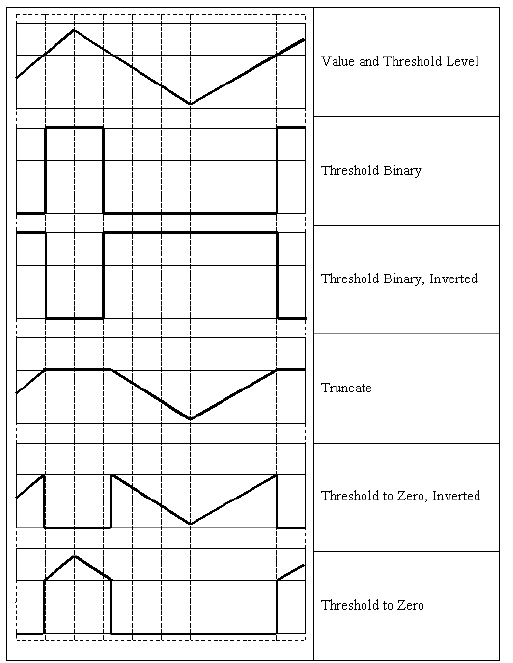
\includegraphics[width=0.5\textwidth]{pics/threshold.png}

See also: \cross{adaptiveThreshold}, \cross{findContours}, \cross{compare}, \cross{min}, \cross{max}

\cvfunc{watershed}\label{watershed}
Does marker-based image segmentation using watershed algrorithm

\begin{lstlisting}
void watershed( const Mat& image, Mat& markers );
\end{lstlisting}
\begin{description}
\cvarg{image}{The input 8-bit 3-channel image.} 
\cvarg{markers}{The input/output 32-bit single-channel image (map) of markers. It should have the same size as \texttt{image}}
\end{description}

The function implements one of the variants
of watershed, non-parametric marker-based segmentation algorithm,
described in \cite{Meyer92}. Before passing the image to the
function, user has to outline roughly the desired regions in the image
\texttt{markers} with positive ($>0$) indices, i.e. every region is
represented as one or more connected components with the pixel values
1, 2, 3 etc (such markers can be retrieved from a binary mask
using \cross{findContours}and \cross{drawContours}, see \texttt{watershed.cpp} demo).
The markers will be "seeds" of the future image
regions. All the other pixels in \texttt{markers}, which relation to the
outlined regions is not known and should be defined by the algorithm,
should be set to 0's. On the output of the function, each pixel in
markers is set to one of values of the "seed" components, or to -1 at
boundaries between the regions.

Note, that it is not necessary that every two neighbor connected
components are separated by a watershed boundary (-1's pixels), for
example, in case when such tangent components exist in the initial
marker image. Visual demonstration and usage example of the function
can be found in OpenCV samples directory; see \texttt{watershed.cpp} demo.

See also: \cross{findContours}


\subsection{Histograms}

\cvfunc{calcHist}\label{calcHist}
Calculates histogram of a set of arrays

\begin{lstlisting}
void calcHist( const Mat* arrays, int narrays,
               const int* channels, const Mat& mask,
               MatND& hist, int dims, const int* histSize,
               const float** ranges, bool uniform=true,
               bool accumulate=false );

void calcHist( const Mat* arrays, int narrays,
               const int* channels, const Mat& mask,
               SparseMat& hist, int dims, const int* histSize,
               const float** ranges, bool uniform=true,
               bool accumulate=false );
\end{lstlisting}
\begin{description}
\cvarg{arrays}{Source arrays. They all should have the same depth, \texttt{CV\_8U} or \texttt{CV\_32F}, and the same size. Each of them can have an arbitrary number of channels}
\cvarg{narrays}{The number of source arrays}
\cvarg{channels}{The list of \texttt{dims} channels that are used to compute the histogram. The first array channels are numerated from 0 to \texttt{arrays[0].channels()-1}, the second array channels are counted from \texttt{arrays[0].channels()} to \texttt{arrays[0].channels() + arrays[1].channels()-1} etc.}
\cvarg{mask}{The optional mask. If the matrix is not empty, it must be 8-bit array of the same size as \texttt{arrays[i]}. The non-zero mask elements mark the array elements that are counted in the histogram}
\cvarg{hist}{The output histogram, a dense or sparse \texttt{dims}-dimensional array}
\cvarg{dims}{The histogram dimensionality; must be positive and not greater than \texttt{CV\_MAX\_DIMS}(=32 in the current OpenCV version)}
\cvarg{histSize}{The array of histogram sizes in each dimension}
\cvarg{ranges}{The array of \texttt{dims} arrays of the histogram bin boundaries in each dimension. When the histogram is uniform (\texttt{uniform}=true), then for each dimension \texttt{i} it's enough to specify the lower (inclusive) boundary $L_0$ of the 0-th histogram bin and the upper (exclusive) boundary $U_{\texttt{histSize}[i]-1}$ for the last histogram bin \texttt{histSize[i]-1}. That is, in the case of uniform histogram each of \texttt{ranges[i]} is an array of 2 elements. When the histogram is not uniform (\texttt{uniform=false}), then each of \texttt{ranges[i]} contains \texttt{histSize[i]+1} elements: $L_0, U_0=L_1, U_1=L_2, ..., U_{\texttt{histSize[i]}-2}=L_{\texttt{histSize[i]}-1}, U_{\texttt{histSize[i]}-1}$. The array elements, which are not between $L_0$ and $U_{\texttt{histSize[i]}-1}$, are not counted in the histogram}
\cvarg{uniform}{Indicates whether the histogram is uniform or not, see above}
\cvarg{accumulate}{Accumulation flag. If it is set, the histogram is not cleared in the beginning (when it is allocated). This feature allows user to compute a single histogram from several sets of arrays, or to update the histogram in time}
\end{description}

The functions \texttt{calcHist} calculate the histogram of one or more
arrays. The elements of a tuple that is used to increment
a histogram bin are taken at the same location from the corresponding
input arrays. The sample below shows how to compute 2D Hue-Saturation histogram for a color imag

\begin{lstlisting}
#include <cv.h>
#include <highgui.h>

using namespace cv;

int main( int argc, char** argv )
{
    Mat src;
    if( argc != 2 || !(src=imread(argv[1], 1)).data )
        return -1;

    Mat hsv;
    cvtColor(src, hsv, CV_BGR2HSV);

    // let's quantize the hue to 30 levels
    // and the saturation to 32 levels
    int hbins = 30, sbins = 32;
    int histSize[] = {hbins, sbins};
    // hue varies from 0 to 179, see cvtColor
    float hranges[] = { 0, 180 };
    // saturation varies from 0 (black-gray-white) to
    // 255 (pure spectrum color)
    float sranges[] = { 0, 256 };
    float* ranges[] = { hranges, sranges };
    MatND hist;
    // we compute the histogram from the 0-th and 1-st channels
    int channels[] = {0, 1};
    
    calcHist( &hsv, 1, channels, Mat(), // do not use mask
        hist, 2, histSize, ranges,
        true, // the histogram is uniform
        false );
    double maxVal=0;
    minMaxLoc(hist, 0, &maxVal, 0, 0);
    
    int scale = 10;
    Mat histImg = Mat::zeros(sbins*scale, hbins*10, CV_8UC3);        

    for( int h = 0; h < hbins; h++ )
        for( int s = 0; s < sbins; s++ )
        {
            float binVal = hist.at<float>(h, s);
            int intensity = cvRound(binVal*255/maxValue);
            cvRectangle( histImg, Point(h*scale, s*scale),
                         Point( (h+1)*scale - 1, (s+1)*scale - 1),
                         Scalar::all(intensity),
                         CV_FILLED );
        }

    namedWindow( "Source", 1 );
    imshow( "Source", src );

    namedWindow( "H-S Histogram", 1 );
    imshow( "H-S Histogram", histImg );

    waitKey();
}
\end{lstlisting}


\cvfunc{calcBackProject}\label{calcBackProject}
Calculates the back projection of a histogram.

\begin{lstlisting}
void calcBackProject( const Mat* arrays, int narrays,
                      const int* channels, const MatND& hist,
                      Mat& backProject, const float** ranges,
                      double scale=1, bool uniform=true );
    
void calcBackProject( const Mat* arrays, int narrays,
                      const int* channels, const SparseMat& hist,
                      Mat& backProject, const float** ranges,
                      double scale=1, bool uniform=true );
\end{lstlisting}
\begin{description}
\cvarg{arrays}{Source arrays. They all should have the same depth, \texttt{CV\_8U} or \texttt{CV\_32F}, and the same size. Each of them can have an arbitrary number of channels}
\cvarg{narrays}{The number of source arrays}
\cvarg{channels}{The list of channels that are used to compute the back projection. The number of channels must match the histogram dimensionality. The first array channels are numerated from 0 to \texttt{arrays[0].channels()-1}, the second array channels are counted from \texttt{arrays[0].channels()} to \texttt{arrays[0].channels() + arrays[1].channels()-1} etc.}
\cvarg{hist}{The input histogram, a dense or sparse}
\cvarg{backProject}{Destination back projection aray; will be a single-channel array of the same size and the same depth as \texttt{arrays[0]}}
\cvarg{ranges}{The array of arrays of the histogram bin boundaries in each dimension. See \cross{calcHist}}
\cvarg{scale}{The optional scale factor for the output back projection}
\cvarg{uniform}{Indicates whether the histogram is uniform or not, see above}
\end{description}

The functions \texttt{calcBackProject} calculate the back project of the histogram. That is, similarly to \texttt{calcHist}, at each location \texttt{(x, y)} the function collects the values from the selected channels in the input images and finds the corresponding histogram bin. But instead of incrementing it, the function reads the bin value, scales it by \texttt{scale} and stores in \texttt{backProject(x,y)}. In terms of statistics, the function computes probability of each element value in respect with the empirical probability distribution represented by the histogram. Here is how, for example, you can find and track a bright-colored object in a scene:

\begin{enumerate}
 \item Before the tracking, show the object to the camera such that covers almost the whole frame. Calculate a hue histogram. The histogram will likely have a strong maximums, corresponding to the dominant colors in the object.
 \item During the tracking, calculate back projection of a hue plane of each input video frame using that pre-computed histogram. Threshold the back projection to suppress weak colors. It may also have sense to suppress pixels with non sufficient color saturation and too dark or too bright pixels.
 \item Find connected components in the resulting picture and choose, for example, the largest component.
\end{enumerate}

That is the approximate algorithm of \cross{CAMShift} color object tracker.

See also: \cross{calcHist}

\cvfunc{compareHist}\label{compareHist}
Compares two histograms

\begin{lstlisting}
double compareHist( const MatND& H1, const MatND& H2, int method );
double compareHist( const SparseMat& H1, const SparseMat& H2, int method );
\end{lstlisting}
\begin{description}
\cvarg{H1}{The first compared histogram}
\cvarg{H2}{The second compared histogram of the same size as \texttt{H1}}
\cvarg{method}{The comparison method, one of the following:
\begin{description}
  \cvarg{CV\_COMP\_CORREL}{Correlation}
  \cvarg{CV\_COMP\_CHISQR}{Chi-Square}
  \cvarg{CV\_COMP\_INTERSECT}{Intersection}
  \cvarg{CV\_COMP\_BHATTACHARYYA}{Bhattacharyya distance}
\end{description}}
\end{description}

The functions \texttt{compareHist} compare two dense or two sparse histograms using the specified method:

\begin{description}
\item[Correlation (method=CV\_COMP\_CORREL)]
\[
d(H_1,H_2) = \frac
{\sum_I (H_1(I) - \bar{H_1}) (H_2(I) - \bar{H_2})}
{\sqrt{\sum_I(H_1(I) - \bar{H_1})^2 \sum_I(H_2(I) - \bar{H_2})^2}}
\]
where
\[
\bar{H_k} = \frac{1}{N} \sum_J H_k(J)
\]
and $N$ is the total number of histogram bins.

\item[Chi-Square (method=CV\_COMP\_CHISQR)]
\[ d(H_1,H_2) = \sum_I \frac{\left(H_1(I)-H_2(I)\right)^2}{H_1(I)+H_2(I)} \]

\item[Intersection (method=CV\_COMP\_INTERSECT)]
\[ d(H_1,H_2) = \sum_I \min (H_1(I), H_2(I)) \]

\item[Bhattacharyya distance (method=CV\_COMP\_BHATTACHARYYA)]
\[ d(H_1,H_2) = \sqrt{1 - \frac{1}{\sqrt{\bar{H_1} \bar{H_2} N^2}} \sum_I \sqrt{H_1(I) \cdot H_2(I)}} \]

\end{description}

The function returns $d(H_1, H_2)$.

While the function works well with 1-, 2-, 3-dimensional dense histograms, it may not be suitable for high-dimensional sparse histograms, where, because of aliasing and sampling problems the coordinates of non-zero histogram bins can slightly shift. To compare such histograms or more general sparse configurations of weighted points, consider using the \cross{calcEMD} function.

\cvfunc{equalizeHist}\label{equalizeHist}
Equalizes the histogram of a grayscale image.

\begin{lstlisting}
void equalizeHist( const Mat& src, Mat& dst );
\end{lstlisting}
\begin{description}
\cvarg{src}{The source 8-bit single channel image}
\cvarg{dst}{The destination image; will have the same size and the same type as \texttt{src}}
\end{description}

The function \texttt{equalizeHist} equalizes the histogram of the input image using the following algorithm:

\begin{enumerate}
\item calculate the histogram $H$ for \texttt{src}.
\item normalize the histogram so that the sum of histogram bins is 255.
\item compute the integral of the histogram:
\[
H'_i = \sum_{0 \le j < i} H(j)
\]
\item transform the image using $H'$ as a look-up table: $\texttt{dst}(x,y) = H'(\texttt{src}(x,y))$
\end{enumerate}

The algorithm normalizes the brightness and increases the contrast of the image.


\subsection{Feature Detection}

\cvfunc{cornerEigenValsAndVecs}\label{cornerEigenValsAndVecs}
Calculates eigenvalues and eigenvectors of image blocks for corner detection.

\begin{lstlisting}
void cornerEigenValsAndVecs( const Mat& src, Mat& dst,
                            int blockSize, int apertureSize,
                            int borderType=BORDER_DEFAULT );
\end{lstlisting}
\begin{description}
\cvarg{src}{Input single-channel 8-bit or floating-point image}
\cvarg{dst}{Image to store the results. It will have the same size as \texttt{src} and the type \texttt{CV\_32FC(6)}}
\cvarg{blockSize}{Neighborhood size (see discussion)}
\cvarg{apertureSize}{Aperture parameter for the \cross{Sobel} operator}
\cvarg{boderType}{Pixel extrapolation method; see \cross{borderInterpolate}}
\end{description}

For every pixel $p$, the function \texttt{cornerEigenValsAndVecs} considers a \texttt{blockSize} $\times$ \texttt{blockSize} neigborhood $S(p)$. It calculates the covariation matrix of derivatives over the neighborhood as:

\[
M = \begin{bmatrix}
\sum_{S(p)}(dI/dx)^2 & \sum_{S(p)}(dI/dx dI/dy)^2 \\
\sum_{S(p)}(dI/dx dI/dy)^2 & \sum_{S(p)}(dI/dy)^2
\end{bmatrix}
\]

Where the derivatives are computed using \cross{Sobel} operator.

After that it finds eigenvectors and eigenvalues of $M$ and stores them into destination image in the form
$(\lambda_1, \lambda_2, x_1, y_1, x_2, y_2)$ where
\begin{description}
\item[$\lambda_1, \lambda_2$]are the eigenvalues of $M$; not sorted
\item[$x_1, y_1$]are the eigenvectors corresponding to $\lambda_1$
\item[$x_2, y_2$]are the eigenvectors corresponding to $\lambda_2$
\end{description}

The output of the function can be used for robust edge or corner detection.

See also: \cross{cornerMinEigenVal}, \cross{cornerHarris}, \cross{preCornerDetect}

\cvfunc{cornerHarris}\label{cornerHarris}
Harris edge detector.

\begin{lstlisting}
void cornerHarris( const Mat& src, Mat& dst, int blockSize,
                  int apertureSize, double k,
                  int borderType=BORDER_DEFAULT );
\end{lstlisting}
\begin{description}
\cvarg{src}{Input single-channel 8-bit or floating-point image}
\cvarg{dst}{Image to store the Harris detector responses; will have type \texttt{CV\_32FC1} and the same size as \texttt{src}}
\cvarg{blockSize}{Neighborhood size (see the discussion of \cross{cornerEigenValsAndVecs})}
\cvarg{apertureSize}{Aperture parameter for the \cross{Sobel} operator}
\cvarg{k}{Harris detector free parameter. See the formula below}
\cvarg{boderType}{Pixel extrapolation method; see \cross{borderInterpolate}}
\end{description}

The function \texttt{cornerHarris} runs the Harris edge detector on the image. Similarly to \cross{cornerMinEigenVal} and \cross{cornerEigenValsAndVecs}, for each pixel $(x, y)$ it calculates a $2\times2$ gradient covariation matrix $M^{(x,y)}$ over a $\texttt{blockSize} \times \texttt{blockSize}$ neighborhood. Then, it computes the following characteristic:

\[
\texttt{dst}(x,y) = \mathrm{det} M^{(x,y)} - k \cdot \left(\mathrm{tr} M^{(x,y)}\right)^2
\]

Corners in the image can be found as the local maxima of this response map.

\cvfunc{cornerMinEigenVal}\label{cornerMinEigenVal}
Calculates the minimal eigenvalue of gradient matrices for corner detection.

\begin{lstlisting}
void cornerMinEigenVal( const Mat& src, Mat& dst,
                        int blockSize, int apertureSize=3,
                        int borderType=BORDER_DEFAULT );
\end{lstlisting}
\begin{description}
\cvarg{src}{Input single-channel 8-bit or floating-point image}
\cvarg{dst}{Image to store the minimal eigenvalues; will have type \texttt{CV\_32FC1} and the same size as \texttt{src}}
\cvarg{blockSize}{Neighborhood size (see the discussion of \cross{cornerEigenValsAndVecs})}
\cvarg{apertureSize}{Aperture parameter for the \cross{Sobel} operator}
\cvarg{boderType}{Pixel extrapolation method; see \cross{borderInterpolate}}
\end{description}

The function \texttt{cornerMinEigenVal} is similar to \cross{cornerEigenValsAndVecs} but it calculates and stores only the minimal eigenvalue of the covariation matrix of derivatives, i.e. $\min(\lambda_1, \lambda_2)$ in terms of the formulae in \cross{cornerEigenValsAndVecs} description.

\cvfunc{cornerSubPix}\label{cornerSubPix}
Refines the corner locations.

\begin{lstlisting}
void cornerSubPix( const Mat& image, vector<Point2f>& corners,
                   Size winSize, Size zeroZone,
                   TermCriteria criteria );
\end{lstlisting}
\begin{description}
\cvarg{image}{Input image}
\cvarg{corners}{Initial coordinates of the input corners; refined coordinates on output}
\cvarg{winSize}{Half of the side length of the search window. For example, if \texttt{winSize=Size(5,5)}, then a 5*2+1 $\times$ 5*2+1 = 11 $\times$ 11 search window would be used}
\cvarg{zeroZone}{Half of the size of the dead region in the middle of the search zone over which the summation in the formula below is not done. It is used sometimes to avoid possible singularities of the autocorrelation matrix. The value of (-1,-1) indicates that there is no such size}
\cvarg{criteria}{Criteria for termination of the iterative process of corner refinement. That is, the process of corner position refinement stops either after a certain number of iterations or when a required accuracy is achieved. The \texttt{criteria} may specify either of or both the maximum number of iteration and the required accuracy}
\end{description}

The function \texttt{cornerSubPix} iterates to find the sub-pixel accurate location of corners, or radial saddle points, as shown in on the picture below.

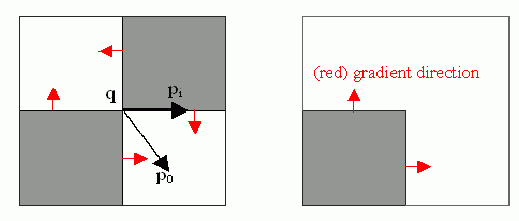
\includegraphics[width=1.0\textwidth]{pics/cornersubpix.png}

Sub-pixel accurate corner locator is based on the observation that every vector from the center $q$ to a point $p$ located within a neighborhood of $q$ is orthogonal to the image gradient at $p$ subject to image and measurement noise. Consider the expression:

\[
\epsilon_i = {DI_{p_i}}^T \cdot (q - p_i)
\]

where ${DI_{p_i}}$ is the image gradient at the one of the points $p_i$ in a neighborhood of $q$. The value of $q$ is to be found such that $\epsilon_i$ is minimized. A system of equations may be set up with $\epsilon_i$ set to zero:

\[
\sum_i(DI_{p_i} \cdot {DI_{p_i}}^T) - \sum_i(DI_{p_i} \cdot {DI_{p_i}}^T \cdot p_i)
\]

where the gradients are summed within a neighborhood ("search window") of $q$. Calling the first gradient term $G$ and the second gradient term $b$ gives:

\[
q = G^{-1} \cdot b
\]

The algorithm sets the center of the neighborhood window at this new center $q$ and then iterates until the center keeps within a set threshold.


\cvfunc{goodFeaturesToTrack}\label{goodFeaturesToTrack}
Determines strong corners on an image.

\begin{lstlisting}
void goodFeaturesToTrack( const Mat& image, vector<Point2f>& corners,
                         int maxCorners, double qualityLevel, double minDistance,
                         const Mat& mask=Mat(), int blockSize=3,
                         bool useHarrisDetector=false, double k=0.04 );
\end{lstlisting}
\begin{description}
\cvarg{image}{The input 8-bit or floating-point 32-bit, single-channel image}
\cvarg{corners}{The output vector of detected corners}
\cvarg{maxCorners}{The maximum number of corners to return. If there are more corners than that will be found, the strongest of them will be returned}
\cvarg{qualityLevel}{Characterizes the minimal accepted quality of image corners; the value of the parameter is multiplied by the by the best corner quality measure (which is the min eigenvalue, see \cross{cornerMinEigenVal}, or the Harris function response, see \cross{cornerHarris}). The corners, which quality measure is less than the product, will be rejected. For example, if the best corner has the quality measure = 1500, and the \texttt{qualityLevel=0.01}, then all the corners which quality measure is less than 15 will be rejected.}
\cvarg{minDistance}{The minimum possible Euclidean distance between the returned corners}
\cvarg{mask}{The optional region of interest. If the image is not empty (then it needs to have the type \texttt{CV\_8UC1} and the same size as \texttt{image}), it will specify the region in which the corners are detected}
\cvarg{blockSize}{Size of the averaging block for computing derivative covariation matrix over each pixel neighborhood, see \cross{cornerEigenValsAndVecs}}
\cvarg{useHarrisDetector}{Indicates, whether to use \hyperref[cornerHarris]{Harris} operator or \cross{cornerMinEigenVal}}
\cvarg{k}{Free parameter of Harris detector}
\end{description}

The function finds the most prominent corners in the image or in the specified image region, as described
in \cite{Shi94}:
\begin{enumerate}
\item the function first calculates the corner quality measure at every source image pixel using the \cross{cornerMinEigenVal} or \cross{cornerHarris}
\item then it performs non-maxima suppression (the local maxima in $3\times 3$ neighborhood
are retained).
\item the next step rejects the corners with the minimal eigenvalue less than $\texttt{qualityLevel} \cdot \max_{x,y} qualityMeasureMap(x,y)$.
\item the remaining corners are then sorted by the quality measure in the descending order.
\item finally, the function throws away each corner $pt_j$ if there is a stronger corner $pt_i$ ($i < j$) such that the distance between them is less than \texttt{minDistance}
\end{enumerate}

The function can be used to initialize a point-based tracker of an object.

See also: \cross{cornerMinEigenVal}, \cross{cornerHarris}, \cross{calcOpticalFlowPyrLK}, \cross{estimateRigidMotion}, \cross{PlanarObjectDetector}, \cross{OneWayDescriptor}

\cvfunc{HoughCircles}\label{HoughCircles}
Finds circles in a grayscale image using a Hough transform.

\begin{lstlisting}
void HoughCircles( Mat& image, vector<Vec3f>& circles,
                 int method, double dp, double minDist,
                 double param1=100, double param2=100,
                 int minRadius=0, int maxRadius=0 );
\end{lstlisting}
\begin{description}
\cvarg{image}{The 8-bit, single-channel, grayscale input image}
\cvarg{circles}{The output vector of found circles. Each vector is encoded as 3-element floating-point vector $(x, y, radius)$}
\cvarg{method}{Currently, the only implemented method is \texttt{CV\_HOUGH\_GRADIENT}, which is basically \emph{21HT}, described in \cite{Yuen90}.}
\cvarg{dp}{The inverse ratio of the accumulator resolution to the image resolution. For example, if \texttt{dp=1}, the accumulator will have the same resolution as the input image, if \texttt{dp=2} - accumulator will have half as big width and height, etc}
\cvarg{minDist}{Minimum distance between the centers of the detected circles. If the parameter is too small, multiple neighbor circles may be falsely detected in addition to a true one. If it is too large, some circles may be missed}
\cvarg{param1}{The first method-specific parameter. in the case of \texttt{CV\_HOUGH\_GRADIENT} it is the higher threshold of the two passed to \cross{Canny} edge detector (the lower one will be twice smaller)}
\cvarg{param2}{The second method-specific parameter. in the case of \texttt{CV\_HOUGH\_GRADIENT} it is the accumulator threshold at the center detection stage. The smaller it is, the more false circles may be detected. Circles, corresponding to the larger accumulator values, will be returned first}
\cvarg{minRadius}{Minimum circle radius}
\cvarg{maxRadius}{Maximum circle radius}
\end{description}

The function \texttt{houghCircles} finds circles in a grayscale image using some modification of Hough transform. Here is a short usage example:

\begin{lstlisting}
#include <cv.h>
#include <highgui.h>
#include <math.h>

using namespace cv;

int main(int argc, char** argv)
{
    Mat img, gray;
    if( argc != 2 && !(img=imread(argv[1], 1)).data)
        return -1;
    cvtColor(img, gray, CV_BGR2GRAY);
    // smooth it, otherwise a lot of false circles may be detected
    GaussianBlur( gray, gray, 9, 9, 2, 2 );
    vector<Vec3f> circles;
    houghCircles(gray, circles, CV_HOUGH_GRADIENT,
                 2, gray->rows/4, 200, 100 );
    for( size_t i = 0; i < circles.size(); i++ )
    {
         Point center(cvRound(circles[i][0]), cvRound(circles[i][1]));
         int radius = cvRound(circles[i][2]);
         // draw the circle center
         circle( img, center, 3, Scalar(0,255,0), -1, 8, 0 );
         // draw the circle outline
         circle( img, center, radius, Scalar(0,0,255), 3, 8, 0 );
    }
    namedWindow( "circles", 1 );
    imshow( "circles", img );
    return 0;
}
\end{lstlisting}

Note that usually the function detects the circles' centers well, however it may fail to find the correct radii. You can assist the function by specifying the radius range (\texttt{minRadius} and \texttt{maxRadius}) if you know it, or you may ignore the returned radius, use only the center and find the correct radius using some additional procedure.

\see also: \cross{fitEllipse}, \cross{minEnclosingCircle}

\cvfunc{HoughLines}\label{HoughLines}
Finds lines in a binary image using standard Hough transform.

\begin{lstlisting}
void HoughLines( Mat& image, vector<Vec2f>& lines,
                 double rho, double theta, int threshold,
                 double srn=0, double stn=0 );
\end{lstlisting}
\begin{description}
\cvarg{image}{The 8-bit, single-channel, binary source image. The image may be modified by the function}
\cvarg{lines}{The output vector of lines. Each line is represented by a two-element vector $(\rho, \theta)$. $\rho$ is the distance from the coordinate origin $(0,0)$ (top-left corner of the image) and $\theta$ is the line rotation angle in radians (0 $\sim$ vertical line, $\pi/2 \sim$ horizontal line)}
\cvarg{rho}{Distance resolution of the accumulator in pixels}
\cvarg{theta}{Angle resolution of the accumulator in radians}
\cvarg{threshold}{The accumulator threshold parameter. Only those lines are returned that get enough votes ($>\texttt{threshold}$)}
\cvarg{srn}{For the multi-scale Hough transform it is the divisor for the distance resolution \texttt{rho}. The coarse accumulator distance resolution will be \texttt{rho} and the accurate accumulator resolution will be \texttt{rho/srn}. If both \texttt{srn=0} and \texttt{stn=0} then the classical Hough transform is used, otherwise both these parameters should be positive.}
\cvarg{stn}{For the multi-scale Hough transform it is the divisor for the distance resolution \texttt{theta}}
\end{description}

The function \texttt{HoughLines} implements standard or standard multi-scale Hough transform algorithm for line detection. See \cross{HoughLinesP} for the code example.


\cvfunc{HoughLinesP}\label{HoughLinesP}
Finds lines segments in a binary image using probabilistic Hough transform.

\begin{lstlisting}
void HoughLinesP( Mat& image, vector<Vec4i>& lines,
                  double rho, double theta, int threshold,
                  double minLineLength=0, double maxLineGap=0 );
\end{lstlisting}
\begin{description}
\cvarg{image}{The 8-bit, single-channel, binary source image. The image may be modified by the function}
\cvarg{lines}{The output vector of lines. Each line is represented by a 4-element vector $(x_1, y_1, x_2, y_2)$, where $(x_1,y_1)$ and $(x_2, y_2)$ are the ending points of each line segment detected.}
\cvarg{rho}{Distance resolution of the accumulator in pixels}
\cvarg{theta}{Angle resolution of the accumulator in radians}
\cvarg{threshold}{The accumulator threshold parameter. Only those lines are returned that get enough votes ($>\texttt{threshold}$)}
\cvarg{minLineLength}{The minimum line length. Line segments shorter than that will be rejected}
\cvarg{maxLineGap}{The maximum allowed gap between points on the same line to link them.}
\end{description}

The function \texttt{HoughLinesP} implements probabilistic Hough transform algorithm for line detection, described in \cite{Matas00}. Below is line detection example:

\begin{lstlisting}
/* This is a standalone program. Pass an image name as a first parameter
of the program.  Switch between standard and probabilistic Hough transform
by changing "#if 1" to "#if 0" and back */
#include <cv.h>
#include <highgui.h>
#include <math.h>

using namespace cv;

int main(int argc, char** argv)
{
    Mat src, dst, color_dst;
    if( argc != 2 || !(src=imread(argv[1], 0)).data)
        return -1;
        
    Canny( src, dst, 50, 200, 3 );
    cvtColor( dst, color_dst, CV_GRAY2BGR );    
        
#if 0
    vector<Vec2f> lines;
    HoughLines( dst, lines, 1, CV_PI/180, 100 );

    for( size_t i = 0; i < lines.size(); i++ )
    {
        float rho = lines[i][0];
        float theta = lines[i][1];
        double a = cos(theta), b = sin(theta);
        double x0 = a*rho, y0 = b*rho;
        Point pt1(cvRound(x0 + 1000*(-b)),
                  cvRound(y0 + 1000*(a)));
        Point pt2(cvRound(x0 - 1000*(-b)),
                  cvRound(y0 - 1000*(a)));
        line( color_dst, pt1, pt2, Scalar(0,0,255), 3, 8 );
    }
#else
    vector<Vec4i> lines;
    HoughLinesP( dst, lines, 1, CV_PI/180, 80, 30, 10 );
    for( size_t i = 0; i < lines.size(); i++ )
    {
        line( color_dst, Point(lines[i][0], lines[i][1]),
            Point(lines[i][2], lines[i][3]), Scalar(0,0,255), 3, 8 );
    }
#endif
    namedWindow( "Source", 1 );
    imshow( "Source", src );

    namedWindow( "Detected Lines", 1 );
    imshow( "Detected Lines", color_dst );

    waitKey(0);
    return 0;
}
\end{lstlisting}


This is the sample picture the function parameters have been tuned for:

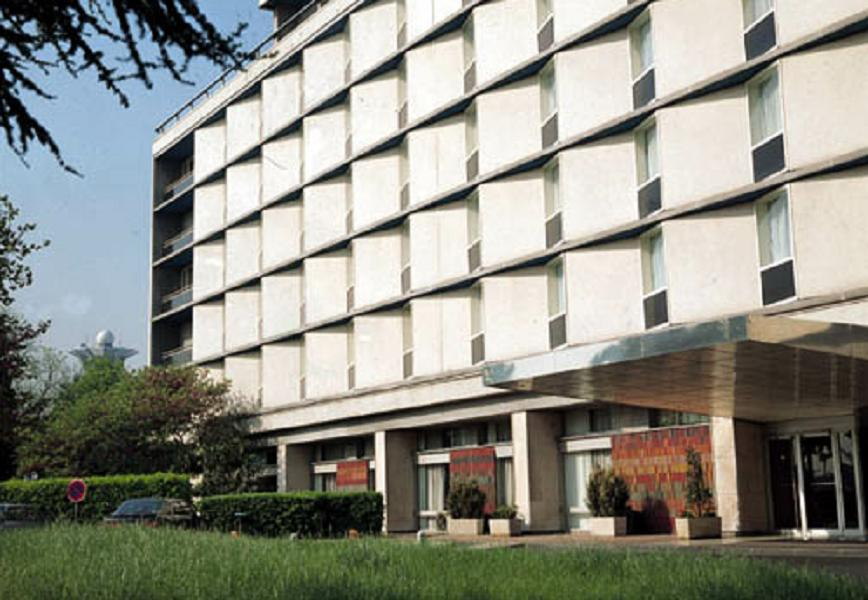
\includegraphics[width=0.5\textwidth]{pics/building.jpg}

And this is the output of the above program in the case of probabilistic Hough transform

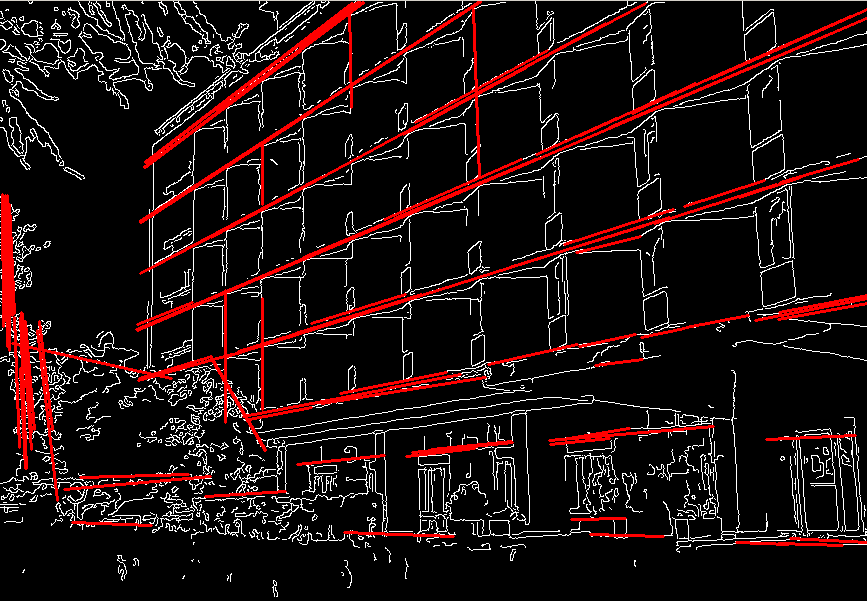
\includegraphics[width=0.5\textwidth]{pics/houghp.png}

\cvfunc{perCornerDetect}\label{perCornerDetect}
Calculates the feature map for corner detection

\begin{lstlisting}
void preCornerDetect( const Mat& src, Mat& dst, int apertureSize,
                     int borderType=BORDER_DEFAULT );
\end{lstlisting}
\begin{description}
\cvarg{src}{The source single-channel 8-bit of floating-point image}
\cvarg{dst}{The output image; will have type \texttt{CV\_32F} and the same size as \texttt{src}}
\cvarg{apertureSize}{Aperture size of \cross{Sobel}}
\cvarg{borderType}{The pixel extrapolation method; see \cross{borderInterpolate}}
\end{description}

The function \texttt{preCornerDetect} calculates the complex spatial derivative-based function of the source image

\[
\texttt{dst} = (D_x \texttt{src})^2 \cdot D_{yy} \texttt{src} + (D_y \texttt{src})^2 \cdot D_{xx} \texttt{src} - 2 D_x \texttt{src} \cdot D_y \texttt{src} \cdot D_{xy} \texttt{src}
\]

where $D_x$, $D_y$ are the first image derivatives, $D_{xx}$, $D_{yy}$ are the second image derivatives and $D_{xy}$ is the mixed derivative.

The corners can be found as local maximums of the functions, as shown below:

\begin{lstlisting}
Mat corners, dilated_corners;
preCornerDetect(image, corners, 3);
// dilation with 3x3 rectangular structuring element
dilate(corners, dilated_corners, Mat(), 1);
Mat corner_mask = corners == dilated_corners;
\end{lstlisting}


\cvfunc{KeyPoint}\label{KeyPoint}
Data structure for salient point detectors

\begin{lstlisting}
class KeyPoint
{
public:
    // default constructor
    KeyPoint();
    // two complete constructors
    KeyPoint(Point2f _pt, float _size, float _angle=-1,
            float _response=0, int _octave=0, int _class_id=-1);
    KeyPoint(float x, float y, float _size, float _angle=-1,
             float _response=0, int _octave=0, int _class_id=-1);
    // coordinate of the point
    Point2f pt;
    // feature size
    float size;
    // feature orintation in degrees
    // (has negative value if the orientation
    // is not defined/not computed)
    float angle;
    // feature strength
    // (can be used to select only
    // the most prominent key points)
    float response;
    // scale-space octave in which the feature has been found;
    // may correlate with the size
    int octave;
    // point class (can be used by feature
    // classifiers or object detectors)
    int class_id;
};

// reading/writing a vector of keypoints to a file storage
void write(FileStorage& fs, const string& name, const vector<KeyPoint>& keypoints);
void read(const FileNode& node, vector<KeyPoint>& keypoints);    
\end{lstlisting}


\cvfunc{MSER}\label{MSER}
Maximally-Stable Extremal Region Extractor

\begin{lstlisting}
class MSER : public CvMSERParams
{
public:
    // default constructor
    MSER();
    // constructor that initializes all the algorithm parameters
    MSER( int _delta, int _min_area, int _max_area,
          float _max_variation, float _min_diversity,
          int _max_evolution, double _area_threshold,
          double _min_margin, int _edge_blur_size );
    // runs the extractor on the specified image; returns the MSERs,
    // each encoded as a contour (vector<Point>, see findContours)
    // the optional mask marks the area where MSERs are searched for
    void operator()(Mat& image, vector<vector<Point> >& msers, const Mat& mask) const;
};
\end{lstlisting}

The class encapsulates all the parameters of MSER (see \url{http://en.wikipedia.org/wiki/Maximally_stable_extremal_regions}) extraction algorithm. 

\cvfunc{SURF}\label{SURF}
Class for extracting Speeded Up Robust Features from an image.

\begin{lstlisting}
class SURF : public CvSURFParams
{
public:
    // default constructor
    SURF();
    // constructor that initializes all the algorithm parameters
    SURF(double _hessianThreshold, int _nOctaves=4,
         int _nOctaveLayers=2, bool _extended=false);
    // returns the number of elements in each descriptor (64 or 128)
    int descriptorSize() const;
    // detects keypoints using fast multi-scale Hessian detector
    void operator()(const Mat& img, const Mat& mask,
                    vector<KeyPoint>& keypoints) const;
    // detects keypoints and computes the SURF descriptors for them
    void operator()(const Mat& img, const Mat& mask,
                    vector<KeyPoint>& keypoints,
                    vector<float>& descriptors,
                    bool useProvidedKeypoints=false) const;
};
\end{lstlisting}

The class \texttt{SURF} implements Speeded Up Robust Features descriptor \cite{Bay06}.
There is fast multi-scale Hessian keypoint detector that can be used to find the keypoints
(which is the default option), but the descriptors can be also computed for the user-specified keypoints.
The function can be used for object tracking and localization, image stitching etc. See the
\texttt{find\_obj.cpp} demo in OpenCV samples directory.


\cvfunc{StarDetector}\label{StarDetector}
Implements Star keypoint detector

\begin{lstlisting}
class StarDetector : CvStarDetectorParams
{
public:
    // default constructor
    StarDetector();
    // the full constructor initialized all the algorithm parameters:
    // maxSize - maximum size of the features. The following 
    //      values of the parameter are supported:
    //      4, 6, 8, 11, 12, 16, 22, 23, 32, 45, 46, 64, 90, 128
    // responseThreshold - threshold for the approximated laplacian,
    //      used to eliminate weak features. The larger it is,
    //      the less features will be retrieved
    // lineThresholdProjected - another threshold for the laplacian to 
    //      eliminate edges
    // lineThresholdBinarized - another threshold for the feature 
    //      size to eliminate edges.
    // The larger the 2 threshold, the more points you get.
    StarDetector(int maxSize, int responseThreshold,
                 int lineThresholdProjected,
                 int lineThresholdBinarized,
                 int suppressNonmaxSize);

    // finds keypoints in an image
    void operator()(const Mat& image, vector<KeyPoint>& keypoints) const;
};
\end{lstlisting}

The class implements a modified version of CenSurE keypoint detector described in
\cite{Agrawal08}

\subsection{Motion Analysis}

\cvfunc{accumulate}\label{accumulate}
Adds image to the accumulator.

\begin{lstlisting}
void accumulate( const Mat& src, Mat& dst, const Mat& mask=Mat() );
\end{lstlisting}
\begin{description}
\cvarg{src}{The input image, 1- or 3-channel, 8-bit or 32-bit floating point}
\cvarg{dst}{The accumulator image with the same number of channels as input image, 32-bit or 64-bit floating-point}
\cvarg{mask}{Optional operation mask}
\end{description}

The function adds \texttt{src}, or some of its elements, to \texttt{dst}:

\[ \texttt{dst}(x,y) \leftarrow \texttt{dst}(x,y) + \texttt{src}(x,y) \quad \text{if} \quad \texttt{mask}(x,y) \ne 0 \]

The function supports multi-channel images; each channel is processed independently.

The functions \texttt{accumulate*} can be used, for example, to collect statistic of background of a scene, viewed by a still camera, for the further foreground-background segmentation.

See also: \cross{accumulateSquare}, \cross{accumulateProduct}, \cross{accumulateWeighted}

\cvfunc{accumulateSquare}\label{accumulateSquare}
Adds the square of the source image to the accumulator.

\begin{lstlisting}
void accumulateSquare( const Mat& src, Mat& dst, const Mat& mask=Mat() );
\end{lstlisting}
\begin{description}
\cvarg{src}{The input image, 1- or 3-channel, 8-bit or 32-bit floating point}
\cvarg{dst}{The accumulator image with the same number of channels as input image, 32-bit or 64-bit floating-point}
\cvarg{mask}{Optional operation mask}
\end{description}

The function \texttt{accumulateSquare} adds the input image \texttt{src} or its selected region, raised to power 2, to the accumulator \texttt{dst}:

\[ \texttt{dst}(x,y) \leftarrow \texttt{dst}(x,y) + \texttt{src}(x,y)^2 \quad \text{if} \quad \texttt{mask}(x,y) \ne 0 \]

The function supports multi-channel images; each channel is processed independently.

See also: \cross{accumulateSquare}, \cross{accumulateProduct}, \cross{accumulateWeighted}

\cvfunc{accumulateProduct}\label{accumulateProduct}
Adds the per-element product of two input images to the accumulator.

\begin{lstlisting}
void accumulateProduct( const Mat& src1, const Mat& src2,
                        Mat& dst, const Mat& mask=Mat() );
\end{lstlisting}
\begin{description}
\cvarg{src1}{The first input image, 1- or 3-channel, 8-bit or 32-bit floating point}
\cvarg{src2}{The second input image of the same type and the same size as \texttt{src1}}
\cvarg{dst}{Accumulator with the same number of channels as input images, 32-bit or 64-bit floating-point}
\cvarg{mask}{Optional operation mask}
\end{description}

The function \texttt{accumulateProduct} adds the product of 2 images or their selected regions to the accumulator \texttt{dst}:

\[ \texttt{dst}(x,y) \leftarrow \texttt{dst}(x,y) + \texttt{src1}(x,y) \cdot \texttt{src2}(x,y) \quad \text{if} \quad \texttt{mask}(x,y) \ne 0 \]

The function supports multi-channel images; each channel is processed independently.

See also: \cross{accumulate}, \cross{accumulateSquare}, \cross{accumulateWeighted}

\cvfunc{accumulateWeighted}\label{accumulateWeighted}
Updates the running average.

\begin{lstlisting}
void accumulateWeighted( const Mat& src, Mat& dst,
                         double alpha, const Mat& mask=Mat() );
\end{lstlisting}
\begin{description}
\cvarg{src}{The input image, 1- or 3-channel, 8-bit or 32-bit floating point}
\cvarg{dst}{The accumulator image with the same number of channels as input image, 32-bit or 64-bit floating-point}
\cvarg{alpha}{Weight of the input image}
\cvarg{mask}{Optional operation mask}
\end{description}

The function \texttt{accumulateWeightedg} calculates the weighted sum of the input image
\texttt{src} and the accumulator \texttt{dst} so that \texttt{dst}
becomes a running average of frame sequence:

\[ \texttt{dst}(x,y) \leftarrow (1-\texttt{alpha}) \cdot \texttt{dst}(x,y) + \texttt{alpha} \cdot \texttt{src}(x,y) \quad \text{if} \quad \texttt{mask}(x,y) \ne 0 \]

that is, \texttt{alpha} regulates the update speed (how fast the accumulator "forgets" about earlier images).
The function supports multi-channel images; each channel is processed independently.

See also: \cross{accumulate}, \cross{accumulateSquare}, \cross{accumulateProduct}

\cvfunc{calcOpticalFlowPyrLK}\label{calcOpticalFlowPyrLK}
Calculates the optical flow for a sparse feature set using the iterative Lucas-Kanade method with pyramids

\begin{lstlisting}
void calcOpticalFlowPyrLK( const Mat& prevImg, const Mat& nextImg,
        const vector<Point2f>& prevPts, vector<Point2f>& nextPts,
        vector<uchar>& status, vector<float>& err, Size winSize=Size(15,15),
        int maxLevel=3, TermCriteria criteria=TermCriteria(
            TermCriteria::COUNT+TermCriteria::EPS, 30, 0.01),
        double derivLambda=0.5, int flags=0 );
enum { OPTFLOW_USE_INITIAL_FLOW=4 };
\end{lstlisting}
\begin{description}
\cvarg{prevImg}{The first 8-bit single-channel or 3-channel input image}
\cvarg{nextImg}{The second input image of the same size and the same type as \texttt{prevImg}}
\cvarg{prevPts}{Vector of points for which the flow needs to be found}
\cvarg{nextPts}{The output vector of points containing the calculated new positions of the input features in the second image}
\cvarg{status}{The output status vector. Each element of the vector is set to 1 if the flow for the corresponding features has been found, 0 otherwise}
\cvarg{err}{The output vector that will contain the difference between patches around the original and moved points}
\cvarg{winSize}{Size of the search window at each pyramid level}
\cvarg{maxLevel}{0-based maximal pyramid level number. If 0, pyramids are not used (single level), if 1, two levels are used etc.}
\cvarg{criteria}{Specifies the termination criteria of the iterative search algorithm (after the specified maximum number of iterations \texttt{criteria.maxCount} or when the search window moves by less than \texttt{criteria.epsilon}}
\cvarg{derivLambda}{The relative weight of the spatial image derivatives impact to the optical flow estimation. If \texttt{derivLambda=0}, only the image intensity is used, if \texttt{derivLambda=1}, only derivatives are used. Any other values between 0 and 1 means that both derivatives and the image intensity are used (in the corresponding proportions).}
\cvarg{flags}{The operation flags:
\begin{description}
  \cvarg{OPTFLOW\_USE\_INITIAL\_FLOW}{use initial estimations stored in \texttt{nextPts}. If the flag is not set, then initially $\texttt{nextPts}\leftarrow\texttt{prevPts}$}
\end{description}}
\end{description}

The function \texttt{calcOpticalFlowPyrLK} implements the sparse iterative version of the Lucas-Kanade optical flow in pyramids, see \cite{Bouguet00}.

\cvfunc{calcOpticalFlowFarneback}\label{calcOpticalFlowFarneback}
Computes dense optical flow using Gunnar Farneback's algorithm

\begin{lstlisting}
void calcOpticalFlowFarneback( const Mat& prevImg, const Mat& nextImg,
                               Mat& flow, double pyrScale, int levels, int winsize,
                               int iterations, int poly_n, double poly_sigma, int flags );
enum { OPTFLOW_FARNEBACK_GAUSSIAN=256 };
\end{lstlisting}
\begin{description}
\cvarg{prevImg}{The first 8-bit single-channel input image}
\cvarg{nextImg}{The second input image of the same size and the same type as \texttt{prevImg}}
\cvarg{flow}{The computed flow image; will have the same size as \texttt{prevImg} and type \texttt{CV\_32FC2}}
\cvarg{pyrScale}{Specifies the image scale (<1) to build the pyramids for each image. \texttt{pyrScale=0.5} means the classical pyramid, where each next layer is twice smaller than the previous}
\cvarg{levels}{The number of pyramid layers, including the initial image. \texttt{levels=1} means that no extra layers are created and only the original images are used}
\cvarg{winsize}{The averaging window size; The larger values increase the algorithm robustness to image noise and give more chances for fast motion detection, but yield more blurred motion field}
\cvarg{iterations}{The number of iterations the algorithm does at each pyramid level}
\cvarg{poly\_n}{Size of the pixel neighborhood used to find polynomial expansion in each pixel. The larger values mean that the image will be approximated with smoother surfaces, yielding more robust algorithm and more blurred  motion field. Typically, \texttt{poly\_n}=5 or 7}
\cvarg{poly\_sigma}{Standard deviation of the Gaussian that is used to smooth derivatives that are used as a basis for the polynomial expansion. For \texttt{poly\_n=5} you can set \texttt{poly\_sigma=1.1}, for \texttt{poly\_n=7} a good value would be \texttt{poly\_sigma=1.5}}
\cvarg{flags}{The operation flags; can be a combination of the following:
\begin{description}
    \cvarg{OPTFLOW\_USE\_INITIAL\_FLOW}{Use the input \texttt{flow} as the initial flow approximation}
    \cvarg{OPTFLOW\_FARNEBACK\_GAUSSIAN}{Use a Gaussian $\texttt{winsize} \times \texttt{winsize}$filter instead of box filter of the same size for optical flow estimation. Usually, this option gives more accurate flow than with a box filter, at the cost of lower speed (and normally \texttt{winsize} for a Gaussian window should be set to a larger value to achieve the same level of robustness)}
\end{description}}
\end{description}

The function finds optical flow for each \texttt{prevImg} pixel using the alorithm so that

\[\texttt{prevImg}(x,y) \sim \texttt{nextImg}(\texttt{flow}(x,y)[0], \texttt{flow}(x,y)[1])\]


\cvfunc{updateMotionHistory}\label{updateMotionHistory}
Updates the motion history image by a moving silhouette.

\begin{lstlisting}
void updateMotionHistory( const Mat& silhouette, Mat& mhi,
                          double timestamp, double duration );
\end{lstlisting}
\begin{description}
\cvarg{silhouette}{Silhouette mask that has non-zero pixels where the motion occurs}
\cvarg{mhi}{Motion history image, that is updated by the function (single-channel, 32-bit floating-point)}
\cvarg{timestamp}{Current time in milliseconds or other units}
\cvarg{duration}{Maximal duration of the motion track in the same units as \texttt{timestamp}}
\end{description}

The function \texttt{updateMotionHistory} updates the motion history image as following:

\[
\texttt{mhi}(x,y)=\forkthree
{\texttt{timestamp}}{if $\texttt{silhouette}(x,y) \ne 0$}
{0}{if $\texttt{silhouette}(x,y) = 0$ and $\texttt{mhi} < (\texttt{timestamp} - \texttt{duration})$}
{\texttt{mhi}(x,y)}{otherwise}
\]
That is, MHI pixels where motion occurs are set to the current \texttt{timestamp}, while the pixels where motion happened last time a long time ago are cleared.

The function, together with \cross{calcMotionGradient} and \cross{calcGlobalOrientation}, implements the motion templates technique, described in \cite{Davis97} and \cite{Bradski00}.
See also the OpenCV sample \texttt{motempl.c} that demonstrates the use of all the motion template functions.

\cvfunc{calcMotionGradient}\label{calcMotionGradient}
Calculates the gradient orientation of a motion history image.

\begin{lstlisting}
void calcMotionGradient( const Mat& mhi, Mat& mask,
                         Mat& orientation,
                         double delta1, double delta2,
                         int apertureSize=3 );
\end{lstlisting}
\begin{description}
\cvarg{mhi}{Motion history single-channel floating-point image}
\cvarg{mask}{The output mask image; will have the type \texttt{CV\_8UC1} and the same size as \texttt{mhi}. Its non-zero elements will mark pixels where the motion gradient data is correct}
\cvarg{orientation}{The output motion gradient orientation image; will have the same type and the same size as \texttt{mhi}. Each pixel of it will the motion orientation in degrees, from 0 to 360.}
\cvarg{delta1, delta2}{The minimal and maximal allowed difference between \texttt{mhi} values within a pixel neighorhood. That is, the function finds the minimum ($m(x,y)$) and maximum ($M(x,y)$) \texttt{mhi} values over $3 \times 3$ neighborhood of each pixel and marks the motion orientation at $(x, y)$ as valid only if
\[
\min(\texttt{delta1} , \texttt{delta2} ) \le M(x,y)-m(x,y) \le \max(\texttt{delta1} ,\texttt{delta2}).
\]}
\cvarg{apertureSize}{The aperture size of \cross{Sobel} operator}
\end{description}

The function \texttt{calcMotionGradient} calculates the gradient orientation at each pixel $(x, y)$ as:

\[
\texttt{orientation}(x,y)=\arctan{\frac{d\texttt{mhi}/dy}{d\texttt{mhi}/dx}}
\]

(in fact, \cross{fastArctan} and \cross{phase} are used, so that the computed angle is measured in degrees and covers the full range 0..360). Also, the \texttt{mask} is filled to indicate pixels where the computed angle is valid.

\cvfunc{calcGlobalOrientation}\label{calcGlobalOrientation}
Calculates the global motion orientation in some selected region.

\begin{lstlisting}
double calcGlobalOrientation( const Mat& orientation, const Mat& mask,
                              const Mat& mhi, double timestamp,
                              double duration );
\end{lstlisting}
\begin{description}
\cvarg{orientation}{Motion gradient orientation image, calculated by the function \cross{calcMotionGradient}}
\cvarg{mask}{Mask image. It may be a conjunction of a valid gradient mask, also calculated by \cross{calcMotionGradient}, and the mask of the region, whose direction needs to be calculated}
\cvarg{mhi}{The motion history image, calculated by \cross{updateMotionHistory}}
\cvarg{timestamp}{The timestamp passed to \cross{updateMotionHistory}}
\cvarg{duration}{Maximal duration of motion track in milliseconds, passed to \cross{updateMotionHistory}}
\end{description}

The function \texttt{calcGlobalOrientation} calculates the average
motion direction in the selected region and returns the angle between
0 degrees  and 360 degrees. The average direction is computed from
the weighted orientation histogram, where a recent motion has larger
weight and the motion occurred in the past has smaller weight, as recorded in \texttt{mhi}.

\cvfunc{CamShift}\label{CamShift}
Finds the object center, size, and orientation

\begin{lstlisting}
RotatedRect CamShift( const Mat& probImage, Rect& window,
                      TermCriteria criteria );
\end{lstlisting}
\begin{description}
\cvarg{probImage}{Back projection of the object histogram; see \cross{calcBackProject}}
\cvarg{window}{Initial search window}
\cvarg{criteria}{Stop criteria for the underlying \cross{meanShift}}
\end{description}

The function \texttt{CamShift} implements the CAMSHIFT object tracking algrorithm
\cross{Bradski98}.
First, it finds an object center using \cross{meanShift} and then adjust the window size and finds the optimal rotation. The function returns the rotated rectangle structure that includes the object position, size and the orientation. The next position of the search window can be obtained with \texttt{RotatedRect::boundingRect()}.

See the OpenCV sample \texttt{camshiftdemo.c} that tracks colored objects.

\cvfunc{meanShift}\label{meanShift}
Finds the object on a back projection image.

\begin{lstlisting}
int meanShift( const Mat& probImage, Rect& window,
               TermCriteria criteria );
\end{lstlisting}
\begin{description}
\cvarg{probImage}{Back projection of the object histogram; see \cross{calcBackProject}}
\cvarg{window}{Initial search window}
\cvarg{criteria}{The stop criteria for the iterative search algorithm}
\end{description}

The function implements iterative object search algorithm. It takes the object back projection on input and the initial position. The mass center in \texttt{window} of the back projection image is computed and the search window center shifts to the mass center. The procedure is repeated until the specified number of iterations \texttt{criteria.maxCount} is done or until the window center shifts by less than \texttt{criteria.epsilon}. The algorithm is used inside \cross{CamShift} and, unlike \cross{CamShift}, the search window size or orientation do not change during the search. You can simply pass the output of \cross{calcBackProject} to this function, but better results can be obtained if you pre-filter the back projection and remove the noise (e.g. by retrieving connected components with \cross{findContours}, throwing away contours with small area (\cross{contourArea}) and rendering the  remaining contours with \cross{drawContours})


\cvfunc{KalmanFilter}\label{KalmanFilter}
Kalman filter class

\begin{lstlisting}
class KalmanFilter
{
public:
    KalmanFilter();
    KalmanFilter(int dynamParams, int measureParams, int controlParams=0);
    void init(int dynamParams, int measureParams, int controlParams=0);

    // predicts statePre from statePost
    const Mat& predict(const Mat& control=Mat());
    // corrects statePre based on the input measurement vector
    // and stores the result to statePost. 
    const Mat& correct(const Mat& measurement);

    Mat statePre;           // predicted state (x'(k)):
                            //    x(k)=A*x(k-1)+B*u(k)
    Mat statePost;          // corrected state (x(k)):
                            //    x(k)=x'(k)+K(k)*(z(k)-H*x'(k))
    Mat transitionMatrix;   // state transition matrix (A)
    Mat controlMatrix;      // control matrix (B)
                            //   (it is not used if there is no control)
    Mat measurementMatrix;  // measurement matrix (H)
    Mat processNoiseCov;    // process noise covariance matrix (Q)
    Mat measurementNoiseCov;// measurement noise covariance matrix (R)
    Mat errorCovPre;        // priori error estimate covariance matrix (P'(k)):
                            //    P'(k)=A*P(k-1)*At + Q)*/
    Mat gain;               // Kalman gain matrix (K(k)):
                            //    K(k)=P'(k)*Ht*inv(H*P'(k)*Ht+R)
    Mat errorCovPost;       // posteriori error estimate covariance matrix (P(k)):
                            //    P(k)=(I-K(k)*H)*P'(k)
    ...
};
\end{lstlisting}

The class implements standard Kalman filter \url{http://en.wikipedia.org/wiki/Kalman_filter}. However, you can modify \texttt{transitionMatrix}, \texttt{controlMatrix} and \texttt{measurementMatrix} to get the extended Kalman filter functionality. See the OpenCV sample \texttt{kalman.c}


\subsection{Structural Analysis and Shape Descriptors}

\cvfunc{moments}\label{moments}
Calculates all of the moments up to the third order of a polygon or rasterized shape.

\begin{lstlisting}
Moments moments( const Mat& array, bool binaryImage=false );

class Moments
{
public:
    Moments();
    Moments(double m00, double m10, double m01, double m20, double m11,
            double m02, double m30, double m21, double m12, double m03 );
    Moments( const CvMoments& moments );
    operator CvMoments() const;
    
    // spatial moments
    double  m00, m10, m01, m20, m11, m02, m30, m21, m12, m03;
    // central moments
    double  mu20, mu11, mu02, mu30, mu21, mu12, mu03;
    // central normalized moments
    double  nu20, nu11, nu02, nu30, nu21, nu12, nu03;
};
\end{lstlisting}
\begin{description}
\cvarg{array}{A raster image (single-channel, 8-bit or floating-point 2D array) or an array
    ($1 \times N$ or $N \times 1$) of 2D points (\texttt{Point} or \texttt{Point2f})}
\cvarg{binaryImage}{(For images only) If it is true, then all the non-zero image pixels are treated as 1's}
\end{description}

The function \texttt{moments} computes moments, up to the 3rd order, of a vector shape or a rasterized shape.
In case of a raster image, the spatial moments $\texttt{Moments::m}_{ji}$ are computed as:

\[\texttt{m}_{ji}=\sum_{x,y} \left(\texttt{array}(x,y) \cdot x^j \cdot y^i\right),\]

the central moments $\texttt{Moments::mu}_{ji}$ are computed as:
\[\texttt{mu}_{ji}=\sum_{x,y} \left(\texttt{array}(x,y) \cdot (x - \bar{x})^j \cdot (y - \bar{y})^i\right)\]
where $(\bar{x}, \bar{y})$ is the mass center:

\[
\bar{x}=\frac{\texttt{m}_{10}}{\texttt{m}_{00}},\; \bar{y}=\frac{\texttt{m}_{01}}{\texttt{m}_{00}}
\]

and the normalized central moments $\texttt{Moments::nu}_{ij}$ are computed as:
\[\texttt{nu}_{ji}=\frac{\texttt{mu}_{ji}}{\texttt{m}_{00}^{(i+j)/2+1}}.\]

Note that $\texttt{mu}_{00}=\texttt{m}_{00}$, $\texttt{nu}_{00}=1$ $\texttt{nu}_{10}=\texttt{mu}_{10}=\texttt{mu}_{01}=\texttt{mu}_{10}=0$, hence the values are not stored.

The moments of a contour are defined in the same way, but computed using Green's formula
(see \url{http://en.wikipedia.org/wiki/Green%27s_theorem}), therefore, because of a limited raster resolution, the moments computed for a contour will be slightly different from the moments computed for the same contour rasterized.

See also: \cross{contourArea}, \cross{arcLength}

\cvfunc{HuMoments}\label{HuMoments}
Calculates the seven Hu invariants.

\begin{lstlisting}
void HuMoments( const Moments& moments, double hu[7] );
\end{lstlisting}
\begin{description}
\cvarg{moments}{The input moments, computed with \cross{moments}}
\cvarg{hu}{The output Hu invariants}
\end{description}

The function \texttt{HuMoments} calculates the seven Hu invariants, see \url{http://en.wikipedia.org/wiki/Image_moment}, that are defined as:

\[ \begin{array}{l}
h[0]=\eta_{20}+\eta_{02}\\
h[1]=(\eta_{20}-\eta_{02})^{2}+4\eta_{11}^{2}\\
h[2]=(\eta_{30}-3\eta_{12})^{2}+ (3\eta_{21}-\eta_{03})^{2}\\
h[3]=(\eta_{30}+\eta_{12})^{2}+ (\eta_{21}+\eta_{03})^{2}\\
h[4]=(\eta_{30}-3\eta_{12})(\eta_{30}+\eta_{12})[(\eta_{30}+\eta_{12})^{2}-3(\eta_{21}+\eta_{03})^{2}]+(3\eta_{21}-\eta_{03})(\eta_{21}+\eta_{03})[3(\eta_{30}+\eta_{12})^{2}-(\eta_{21}+\eta_{03})^{2}]\\
h[5]=(\eta_{20}-\eta_{02})[(\eta_{30}+\eta_{12})^{2}- (\eta_{21}+\eta_{03})^{2}]+4\eta_{11}(\eta_{30}+\eta_{12})(\eta_{21}+\eta_{03})\\
h[6]=(3\eta_{21}-\eta_{03})(\eta_{21}+\eta_{03})[3(\eta_{30}+\eta_{12})^{2}-(\eta_{21}+\eta_{03})^{2}]-(\eta_{30}-3\eta_{12})(\eta_{21}+\eta_{03})[3(\eta_{30}+\eta_{12})^{2}-(\eta_{21}+\eta_{03})^{2}]\\
\end{array}
\]

where $\eta_{ji}$ stand for $\texttt{Moments::nu}_{ji}$.

These values are proved to be invariant to the image scale, rotation, and reflection except the seventh one, whose sign is changed by reflection. Of course, this invariance was proved with the assumption of infinite image resolution. In case of a raster images the computed Hu invariants for the original and transformed images will be a bit different.

See also: \cross{matchShapes}

\cvfunc{findContours}\label{findContours}
Finds the contours in a binary image.

\begin{lstlisting}
void findContours( const Mat& image, vector<vector<Point> >& contours,
                   vector<Vec4i>& hierarchy, int mode,
                   int method, Point offset=Point());

void findContours( const Mat& image, vector<vector<Point> >& contours,
                   int mode, int method, Point offset=Point());

enum { RETR_EXTERNAL=CV_RETR_EXTERNAL, RETR_LIST=CV_RETR_LIST,
      RETR_CCOMP=CV_RETR_CCOMP, RETR_TREE=CV_RETR_TREE };

enum { CHAIN_APPROX_NONE=CV_CHAIN_APPROX_NONE,
      CHAIN_APPROX_SIMPLE=CV_CHAIN_APPROX_SIMPLE,
      CHAIN_APPROX_TC89_L1=CV_CHAIN_APPROX_TC89_L1,
      CHAIN_APPROX_TC89_KCOS=CV_CHAIN_APPROX_TC89_KCOS };
\end{lstlisting}
\begin{description}
\cvarg{image}{The source, an 8-bit single-channel image. Non-zero pixels are treated as 1's, zero pixels remain 0's - the image is treated as \texttt{binary}. You can use \cross{compare}, \cross{inRange}, \cross{threshold}, \cross{adaptiveThreshold}, \cross{Canny} etc. to create a binary image out of a grayscale or color one. The function modifies the \texttt{image} while extracting the contours}
\cvarg{contours}{The detected contours. Each contour is stored as a vector of points}
\cvarg{hiararchy}{The optional output vector that will contain information about the image topology. It will have as many elements as the number of contours. For each contour \texttt{contours[i]}, the elements \texttt{hierarchy[i][0]}, \texttt{hiearchy[i][1]}, \texttt{hiearchy[i][2]}, \texttt{hiearchy[i][3]} will be set to 0-based indices in \texttt{contours} of the next and previous contours at the same hierarchical level, the first child contour and the parent contour, respectively. If for some contour \texttt{i} there is no next, previous, parent or nested contours, the corresponding elements of \texttt{hierarchy[i]} will be negative}
\cvarg{mode}{The contour retrieval mode
\begin{description}
  \cvarg{RETR\_EXTERNAL}{retrieves only the extreme outer contours; It will set \texttt{hierarchy[i][2]=hierarchy[i][3]=-1} for all the contours}
  \cvarg{RETR\_LIST}{retrieves all of the contours without establishing any hierarchical relationships}
  \cvarg{RETR\_CCOMP}{retrieves all of the contours and organizes them into a two-level hierarchy: on the top level are the external boundaries of the components, on the second level are the boundaries of the holes. If inside a hole of a connected component there is another contour, it will still be put on the top level}
  \cvarg{CV\_RETR\_TREE}{retrieves all of the contours and reconstructs the full hierarchy of nested contours. This full hierarchy is built and shown in OpenCV \texttt{contours.c} demo}
\end{description}}
\cvarg{method}{The contour approximation method.
\begin{description}
  \cvarg{CV\_CHAIN\_APPROX\_NONE}{stores absolutely all the contour points. That is, every 2 points of a contour stored with this method are 8-connected neighbors of each other}
  \cvarg{CV\_CHAIN\_APPROX\_SIMPLE}{compresses horizontal, vertical, and diagonal segments and leaves only their end points. E.g. an up-right rectangular contour will be encoded with 4 points}
  \cvarg{CV\_CHAIN\_APPROX\_TC89\_L1,CV\_CHAIN\_APPROX\_TC89\_KCOS}{applies one of the flavors of the Teh-Chin chain approximation algorithm; see \cite{TehChin89}}
\end{description}}
\cvarg{offset}{The optional offset, by which every contour point is shifted. This is useful if the contours are extracted from the image ROI and then they should be analyzed in the whole image context}
\end{description}

The function \texttt{findContours} retrieves contours from the
binary image using the algorithm \cite{Suzuki85}. The contours are a useful tool for shape analysis and object detection and recognition. See \texttt{squares.c} in the OpenCV sample directory.

\cvfunc{drawContours}\label{drawContours}
Draws contours' outlines or filled contours.

\begin{lstlisting}
void drawContours( Mat& image, const vector<vector<Point> >& contours,
                   int contourIdx, const Scalar& color, int thickness=1,
                   int lineType=8, const vector<Vec4i>& hierarchy=vector<Vec4i>(),
                   int maxLevel=INT_MAX, Point offset=Point() );
\end{lstlisting}
\begin{description}
\cvarg{image}{The destination image}
\cvarg{contours}{All the input contours. Each contour is stored as a point vector}
\cvarg{contourIdx}{Indicates the contour to draw. If it is negative, all the contours are drawn}
\cvarg{color}{The contours' color}
\cvarg{thickness}{Thickness of lines the contours are drawn with.
If it is negative (e.g. \texttt{thickness=CV\_FILLED}), the contour interiors are
drawn.}
\cvarg{lineType}{The line connectivity; see \cross{line} description}
\cvarg{hierarchy}{The optional information about hierarchy. It is only needed if you want to draw only some of the  contours (see \texttt{maxLevel})}
\cvarg{maxLevel}{Maximal level for drawn contours. If 0, only
the specified contour is drawn. If 1, the function draws the contour(s) and all the nested contours. If 2, the function draws the contours, all the nested contours and all the nested into nested contours etc. This parameter is only taken into account when there is \texttt{hierarchy} available.}
\cvarg{offset}{The optional contour shift parameter. Shift all the drawn contours by the specified $\texttt{offset}=(dx,dy)$}

The function \texttt{drawContours} draws contour outlines in the image if $\texttt{thickness} \ge 0$ or fills the area bounded by the contours if $ \texttt{thickness}<0$. Here is the example on how to retrieve connected components from the binary image and label them

\begin{lstlisting}
#include "cv.h"
#include "highgui.h"

using namespace cv;

int main( int argc, char** argv )
{
    Mat src;
    // the first command line parameter must be file name of binary 
    // (black-n-white) image
    if( argc != 2 || !(src=imread(argv[1], 0)).data)
        return -1;

    Mat dst = Mat::zeros(src.rows, src.cols, CV_8UC3);

    src = src > 1;
    namedWindow( "Source", 1 );
    imshow( "Source", src );

    vector<vector<Point> > contours;
    vector<Vec4i> hierarchy;
    
    findContours( src, contours, hierarchy, 
        CV_RETR_CCOMP, CV_CHAIN_APPROX_SIMPLE );

    // iterate through all the top-level contours,
    // draw each connected component with its own random color
    int idx = 0;
    for( ; idx >= 0; idx = hiearchy[idx][0] )
    {
        Scalar color( rand()&255, rand()&255, rand()&255 );
        drawContours( dst, contours, idx, color, CV_FILLED, 8, hiearchy );
    }

    namedWindow( "Components", 1 );
    showImage( "Components", dst );
    waitKey(0);
}
\end{lstlisting}


\cvfunc{approxPolyDP}\label{approxPolyDP}
Approximates polygonal curve(s) with the specified precision.

\begin{lstlisting}
void approxPolyDP( const Mat& curve,
                   vector<Point>& approxCurve,
                   double epsilon, bool closed );
void approxPolyDP( const Mat& curve,
                   vector<Point2f>& approxCurve,
                   double epsilon, bool closed );
\end{lstlisting}
\begin{description}
\cvarg{curve}{The polygon or curve to approximate. Must be $1 \times N$ or $N \times 1$ matrix of type \texttt{CV\_32SC2} or \texttt{CV\_32FC2}. You can also pass \texttt{vector<Point>} or \texttt{vector<Point2f} that will be automatically converted to the matrix of the proper size and type}
\cvarg{approxCurve}{The result of the approximation; The type should match the type of the input curve}
\cvarg{epsilon}{Specifies the approximation accuracy. This is the maximum distance between the original curve and its approximation}
\cvarg{closed}{If true, the approximated curve is closed (i.e. its first and last vertices are connected), otherwise it's not}
\end{description}

The functions \texttt{approxPolyDP} approximate a curve or a polygon with another curve/polygon with less vertices, so that the distance between them is less or equal to the specified precision. It used Douglas-Peucker algorithm \url{http://en.wikipedia.org/wiki/Ramer-Douglas-Peucker_algorithm}

\cvfunc{arcLength}\label{arcLength}
Calculates a contour perimeter or a curve length.

\begin{lstlisting}
double arcLength( const Mat& curve, bool closed );
\end{lstlisting}
\begin{description}
\cvarg{curve}{The input vector of 2D points, represented by \texttt{CV\_32SC2} or \texttt{CV\_32FC2} matrix or by \texttt{vector<Point>} or \texttt{vector<Point2f>}}
\cvarg{closed}{Indicates, whether the curve is closed or not}
\end{description}

The function computes the curve length or the closed contour perimeter.

\cvfunc{boundingRect}\label{boundingRect}
Calculates the up-right bounding rectangle of a point set.

\begin{lstlisting}
Rect boundingRect( const Mat& points );
\end{lstlisting}
\begin{description}
\cvarg{points}{The input 2D point set, represented by \texttt{CV\_32SC2} or \texttt{CV\_32FC2} matrix or by \texttt{vector<Point>} or \texttt{vector<Point2f>}}
\end{description}

The function calculates and returns the minimal up-right bounding rectangle for the specified point set.


\cvfunc{estimateRigidTransform}\label{estimateRigidTransform}
Computes optimal affine transformation between two 2D point sets

\begin{lstlisting}
Mat estimateRigidTransform( const Mat& srcpt, const Mat& dstpt,
                            bool fullAffine );
\end{lstlisting}
\begin{description}
\cvarg{srcpt}{The first input 2D point set}
\cvarg{dst}{The second input 2D point set of the same size and the same type as \texttt{A}}
\cvarg{fullAffine}{If true, the function finds the optimal affine transformation with no any additional resrictions (i.e. there are 6 degrees of freedom); otherwise, the class of transformations to choose from is limited to combinations of translation, rotation and uniform scaling (i.e. there are 5 degrees of freedom)}
\end{description}

The function finds the optimal affine transform $[A|b]$ (a $2 \times 3$ floating-point matrix) that approximates best the transformation from $\texttt{srcpt}_i$ to $\texttt{dstpt}_i$:

\[ [A^*|b^*] = arg \min_{[A|b]} \sum_i \|\texttt{dstpt}_i - A {\texttt{srcpt}_i}^T - b \|^2 \]

where $[A|b]$ can be either arbitrary (when \texttt{fullAffine=true}) or have form
$\begin{bmatrix}a_{11} & a_{12} & b_1 \\ -a_{12} & a_{11} & b_2 \end{bmatrix}$ when \texttt{fullAffine=false}.

See also: \cross{getAffineTransform}, \cross{getPerspectiveTransform}, \cross{findHomography}

\cvfunc{estimateAffine3D}\label{estimateAffine3D}
Computes optimal affine transformation between two 3D point sets

\begin{lstlisting}
int estimateAffine3D(const Mat& srcpt, const Mat& dstpt, Mat& out,
                     vector<uchar>& outliers,
                     double ransacThreshold = 3.0,
                     double confidence = 0.99);
\end{lstlisting}
\begin{description}
\cvarg{srcpt}{The first input 3D point set}
\cvarg{dstpt}{The second input 3D point set}
\cvarg{out}{The output 3D affine transformation matrix $3 \times 4$}
\cvarg{outliers}{The output vector indicating which points are outliers}
\cvarg{ransacThreshold}{The maximum reprojection error in RANSAC algorithm to consider a point an inlier}
\cvarg{confidence}{The confidence level, between 0 and 1, with which the matrix is estimated}
\end{description}

The function estimates the optimal 3D affine transformation between two 3D point sets using RANSAC algorithm.


\cvfunc{contourArea}\label{contourArea}
Calculates the contour area

\begin{lstlisting}
double contourArea( const Mat& contour );    
\end{lstlisting}
\begin{description}
\cvarg{contour}{The contour vertices, represented by \texttt{CV\_32SC2} or \texttt{CV\_32FC2} matrix or by \texttt{vector<Point>} or \texttt{vector<Point2f>}}
\end{description}

The function computes the contour area. Similarly to \cross{moments} the area is computed using the Green formula, thus the returned area and the number of non-zero pixels, if you draw the contour using \cross{drawContours} or \cross{fillPoly}, can be different.
Here is a short example:

\begin{lstlisting}
vector<Point> contour;
contour.push_back(Point2f(0, 0));
contour.push_back(Point2f(10, 0));
contour.push_back(Point2f(10, 10));
contour.push_back(Point2f(5, 4));

double area0 = contourArea(contour);
vector<Point> approx;
approxPolyDP(contour, approx, 5, true);
double area1 = contourArea(approx);

cout << "area0 =" << area0 << endl <<
        "area1 =" << area1 << endl <<
        "approx poly vertices" << approx.size() << endl; 
\end{lstlisting}

\cvfunc{convexHull}    
Finds the convex hull of a point set.

\begin{lstlisting}
void convexHull( const Mat& points, vector<int>& hull,
                 bool clockwise=false );
void convexHull( const Mat& points, vector<Point>& hull,
                 bool clockwise=false );
void convexHull( const Mat& points, vector<Point2f>& hull,
                 bool clockwise=false );
\end{lstlisting}
\begin{description}
\cvarg{points}{The input 2D point set, represented by \texttt{CV\_32SC2} or \texttt{CV\_32FC2} matrix or by
\texttt{vector<Point>} or \texttt{vector<Point2f>}}
\cvarg{hull}{The output convex hull. It is either a vector of points that form the hull, or a vector of 0-based point indices of the hull points in the original array (since the set of convex hull points is a subset of the original point set).}
\cvarg{clockwise}{If true, the output convex hull will be oriented clockwise, otherwise it will be oriented counter-clockwise. Here, the usual screen coordinate system is assumed - the origin is at the top-left corner, x axis is oriented to the right, and y axis is oriented downwards.}
\end{description}

The functions find the convex hull of a 2D point set using Sklansky's algorithm \cite{Sklansky82} that has $O(N logN)$ or $O(N)$ complexity (where $N$ is the number of input points), depending on how the initial sorting is implemented (currently it is $O(N logN)$. See the OpenCV sample \texttt{convexhull.c} that demonstrates the use of the different function variants. 

\cvfunc{findHomography}\label{findHomography}
Finds the optimal perspective transformation between two 2D point sets

\begin{lstlisting}
Mat findHomography( const Mat& srcPoints, const Mat& dstPoints,
                    Mat& mask, int method=0,
                    double ransacReprojThreshold=0 );
    
Mat findHomography( const Mat& srcPoints, const Mat& dstPoints,
                    vector<uchar>& mask, int method=0,
                    double ransacReprojThreshold=0 );

Mat findHomography( const Mat& srcPoints, const Mat& dstPoints,
                    int method=0, double ransacReprojThreshold=0 );
enum { LMEDS=4, RANSAC=8 };
\end{lstlisting}
\begin{description}
\cvarg{srcPoints}{Coordinates of the points in the original plane, a matrix of type \texttt{CV\_32FC2} or a \texttt{vector<Point2f>}.}
\cvarg{dstPoints}{Coordinates of the points in the target plane, a matrix of type \texttt{CV\_32FC2} or a \texttt{vector<Point2f>}.}
\cvarg{method}{The method used to compute the homography matrix; one of the following:
\begin{description}
\cvarg{0}{regular method using all the point pairs}
\cvarg{RANSAC}{RANSAC-based robust method}
\cvarg{LMEDS}{Least-Median robust method}
\end{description}}
\cvarg{ransacReprojThreshold}{The maximum allowed reprojection error to treat a point pair as an inlier (used in the RANSAC method only). That is, if
\[\|\texttt{dstPoints}_i - \texttt{convertPointHomogeneous}(\texttt{H} \texttt{srcPoints}_i)\| > \texttt{ransacReprojThreshold}\]
then the point $i$ is considered an outlier. If \texttt{srcPoints} and \texttt{dstPoints} are measured in pixels, it usually makes sense to set this parameter somewhere in the range 1 to 10. }
\cvarg{mask}{The optional output mask 8-bit single-channel matrix or a vector; will have as many elements as \texttt{srcPoints}. \texttt{mask[i]} is set to 0 if the point $i$ is outlier and 0 otherwise}
\end{description}

The functions \texttt{findHomography} find and return the perspective transformation $H$ between the source and the destination planes:

\[
s_i \vecthree{x'_i}{y'_i}{1} \sim H \vecthree{x_i}{y_i}{1}
\]

So that the back-projection error

\[
\sum_i
\left( x'_i-\frac{h_{11} x_i + h_{12} y_i + h_{13}}{h_{31} x_i + h_{32} y_i + h_{33}} \right)^2+
\left( y'_i-\frac{h_{21} x_i + h_{22} y_i + h_{23}}{h_{31} x_i + h_{32} y_i + h_{33}} \right)^2
\]

is minimized. If the parameter method is set to the default value 0, the function
uses all the point pairs and estimates the best suitable homography
matrix. However, if not all of the point pairs ($src\_points_i$,
$dst\_points_i$) fit the rigid perspective transformation (i.e. there
can be outliers), it is still possible to estimate the correct
transformation using one of the robust methods available. Both
methods, \texttt{RANSAC} and \texttt{LMEDS}, try many different random subsets
of the corresponding point pairs (of 4 pairs each), estimate
the homography matrix using this subset and a simple least-square
algorithm and then compute the quality/goodness of the computed homography
(which is the number of inliers for RANSAC or the median reprojection
error for LMeDs). The best subset is then used to produce the initial
estimate of the homography matrix and the mask of inliers/outliers.

Regardless of the method, robust or not, the computed homography
matrix is refined further (using inliers only in the case of a robust
method) with the Levenberg-Marquardt method in order to reduce the
reprojection error even more.

The method \texttt{RANSAC} can handle practically any ratio of outliers,
but it needs the threshold to distinguish inliers from outliers.
The method \texttt{LMEDS} does not need any threshold, but it works
correctly only when there are more than 50\% of inliers. Finally,
if you are sure in the computed features and there can be only some
small noise, but no outliers, the default method could be the best
choice.

The function is used to find initial intrinsic and extrinsic matrices.
Homography matrix is determined up to a scale, thus it is normalized
to make $h_{33} =1$.

See also: \cross{getAffineTransform}, \cross{getPerspectiveTransform}, \cross{estimateRigidMotion},
\cross{warpPerspective}


\cvfunc{fitEllipse}\label{fitEllipse}
Fits an ellipse around a set of 2D points.

\begin{lstlisting}
RotatedRect fitEllipse( const Mat& points );
\end{lstlisting}
\begin{description}
\cvarg{points}{The input 2D point set, represented by \texttt{CV\_32SC2} or \texttt{CV\_32FC2} matrix or by
\texttt{vector<Point>} or \texttt{vector<Point2f>}}
\end{description}

The function \texttt{fitEllipse} calculates the ellipse that fits best
(in least-squares sense) a set of 2D points. It returns the rotated rectangle in which the ellipse is inscribed.

\cvfunc{fitLine}\label{fitLine}
Fits a line to a 2D or 3D point set.

\begin{lstlisting}
void fitLine( const Mat& points, Vec4f& line, int distType,
              double param, double reps, double aeps );
void fitLine( const Mat& points, Vec6f& line, int distType,
              double param, double reps, double aeps );
\end{lstlisting}
\begin{description}
\cvarg{points}{The input 2D point set, represented by \texttt{CV\_32SC2} or \texttt{CV\_32FC2} matrix or by
\texttt{vector<Point>}, \texttt{vector<Point2f>}, \texttt{vector<Point3i>} or \texttt{vector<Point3f>}}
\cvarg{line}{The output line parameters. In the case of a 2d fitting,
it is a vector of 4 floats \texttt{(vx, vy,
x0, y0)} where \texttt{(vx, vy)} is a normalized vector collinear to the
line and \texttt{(x0, y0)} is some point on the line. in the case of a
3D fitting it is vector of 6 floats \texttt{(vx, vy, vz, x0, y0, z0)}
where \texttt{(vx, vy, vz)} is a normalized vector collinear to the line
and \texttt{(x0, y0, z0)} is some point on the line}
\cvarg{distType}{The distance used by the M-estimator (see the discussion)}
\cvarg{param}{Numerical parameter (\texttt{C}) for some types of distances, if 0 then some optimal value is chosen}
\cvarg{reps, aeps}{Sufficient accuracy for the radius (distance between the coordinate origin and the line) and angle, respectively; 0.01 would be a good default value for both.}
\end{description}

The functions \texttt{fitLine} fit a line to a 2D or 3D point set by minimizing $\sum_i \rho(r_i)$ where $r_i$ is the distance between the $i^{th}$ point and the line and $\rho(r)$ is a distance function, one of:

\begin{description}
\item[distType=CV\_DIST\_L2]
\[ \rho(r) = r^2/2 \quad \text{(the simplest and the fastest least-squares method)} \]

\item[distType=CV\_DIST\_L1]
\[ \rho(r) = r \]

\item[distType=CV\_DIST\_L12]
\[ \rho(r) = 2 \cdot (\sqrt{1 + \frac{r^2}{2}} - 1) \]

\item[distType=CV\_DIST\_FAIR]
\[ \rho\left(r\right) = C^2 \cdot \left( \frac{r}{C} - \log{\left(1 + \frac{r}{C}\right)}\right) \quad \text{where} \quad C=1.3998 \]

\item[distType=CV\_DIST\_WELSCH]
\[ \rho\left(r\right) = \frac{C^2}{2} \cdot \left( 1 - \exp{\left(-\left(\frac{r}{C}\right)^2\right)}\right) \quad \text{where} \quad C=2.9846 \]

\item[distType=CV\_DIST\_HUBER]
\[ \rho(r) = \fork
{r^2/2}{if $r < C$}
{C \cdot (r-C/2)}{otherwise}  \quad \text{where} \quad C=1.345
\]
\end{description}

The algorithm is based on the M-estimator (\url{http://en.wikipedia.org/wiki/M-estimator}) technique, that iteratively fits the line using weighted least-squares algorithm and after each iteration the weights $w_i$ are adjusted to beinversely proportional to $\rho(r_i)$. 


\cvfunc{isContourConvex}\label{isContourConvex}
Tests contour convexity.

\begin{lstlisting}
bool isContourConvex( const Mat& contour );
\end{lstlisting}
\begin{description}
\cvarg{contour}{The tested contour, a matrix of type \texttt{CV\_32SC2} or \texttt{CV\_32FC2}, or \texttt{vector<Point>} or \texttt{vector<Point2f>}}
\end{description}

The function \texttt{isContourConvex} tests whether the input contour is convex or not. The contour must be simple, i.e. without self-intersections, otherwise the function output is undefined.


\cvfunc{minAreaRect}\label{minAreaRect}
Finds the minimum area rotated rectangle enclosing a 2D point set.

\begin{lstlisting}
RotatedRect minAreaRect( const Mat& points );
\end{lstlisting}
\begin{description}
\cvarg{points}{The input 2D point set, represented by \texttt{CV\_32SC2} or \texttt{CV\_32FC2} matrix or by \texttt{vector<Point>} or \texttt{vector<Point2f>}}
\end{description}

The function calculates and returns the minimum area bounding rectangle (possibly rotated) for the specified point set. See the OpenCV sample \texttt{minarea.c}

\cvfunc{minEnclosingCircle}\label{minEnclosingCircle}
Finds the minimum area circle enclosing a 2D point set.

\begin{lstlisting}
void minEnclosingCircle( const Mat& points, Point2f& center, float& radius );    
\end{lstlisting}
\begin{description}
\cvarg{points}{The input 2D point set, represented by \texttt{CV\_32SC2} or \texttt{CV\_32FC2} matrix or by \texttt{vector<Point>} or \texttt{vector<Point2f>}}
\cvarg{center}{The output center of the circle}
\cvarg{radius}{The output radius of the circle}
\end{description}

The function finds the minimal enclosing circle of a 2D point set using iterative algorithm. See the OpenCV sample \texttt{minarea.c}

\cvfunc{matchShapes}\label{matchShapes}
Compares two shapes.

\begin{lstlisting}
double matchShapes( const Mat& object1,
                    const Mat& object2,
                    int method, double parameter=0 );
\end{lstlisting}
\begin{description}
\cvarg{object1}{The first contour or grayscale image}
\cvarg{object2}{The second contour or grayscale image}
\cvarg{method}{Comparison method:
 \texttt{CV\_CONTOUR\_MATCH\_I1},\\ 
 \texttt{CV\_CONTOURS\_MATCH\_I2}\\ 
or 
 \texttt{CV\_CONTOURS\_MATCH\_I3} (see the discussion below)}
\cvarg{parameter}{Method-specific parameter (is not used now)}
\end{description}

The function \texttt{matchShapes} compares two shapes. The 3 implemented methods all use Hu invariants (see \cross{HuMoments}) as following ($A$ denotes \texttt{object1}, $B$ denotes \texttt{object2}):

\begin{description}
\item[method=CV\_CONTOUR\_MATCH\_I1]
\[ I_1(A,B) = \sum_{i=1...7} \left| \frac{1}{m^A_i} - \frac{1}{m^B_i} \right| \]

\item[method=CV\_CONTOUR\_MATCH\_I2]
\[ I_2(A,B) = \sum_{i=1...7} \left| m^A_i - m^B_i \right| \]

\item[method=CV\_CONTOUR\_MATCH\_I3]
\[ I_3(A,B) = \sum_{i=1...7} \frac{ \left| m^A_i - m^B_i \right| }{ \left| m^A_i \right| } \]
\end{description}

where

\[
\begin{array}{l}
m^A_i = \mathrm{sign}(h^A_i) \cdot \log{h^A_i} \\
m^B_i = \mathrm{sign}(h^B_i) \cdot \log{h^B_i}
\end{array}
\]

and $h^A_i, h^B_i$ are the Hu moments of $A$ and $B$ respectively.


\cvfunc{pointPolygonTest}\label{pointPolygonTest}
Performs point-in-contour test.

\begin{lstlisting}
double pointPolygonTest( const Mat& contour,
                         Point2f pt, bool measureDist );
\end{lstlisting}
\begin{description}
\cvarg{contour}{The input contour}
\cvarg{pt}{The point tested against the contour}
\cvarg{measureDist}{If true, the function estimates the signed distance from the point to the nearest contour edge; otherwise, the function only checks if the point is inside or not.}
\end{description}

The function determines whether the
point is inside a contour, outside, or lies on an edge (or coincides
with a vertex). It returns positive (inside), negative (outside) or zero (on an edge) value,
correspondingly. When \texttt{measureDist=false}, the return value
is +1, -1 and 0, respectively. Otherwise, the return value
it is a signed distance between the point and the nearest contour
edge.

Here is the sample output of the function, where each image pixel is tested against the contour.

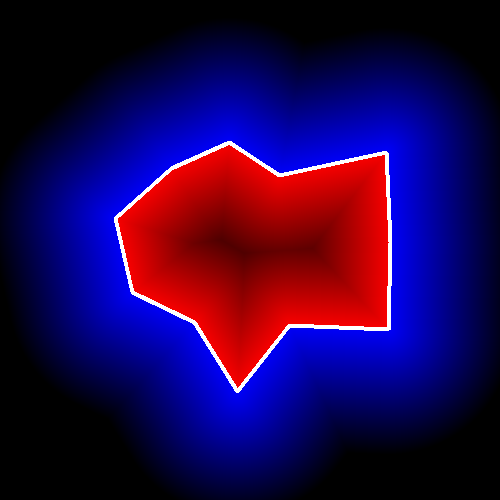
\includegraphics[width=0.5\textwidth]{pics/pointpolygon.png}

\subsection{Object Detection}

\cvfunc{FeatureEvaluator}\label{FeatureEvaluator}
Base class for computing feature values in cascade classifiers

\begin{lstlisting}
class FeatureEvaluator
{
public:    
    // feature type
    enum { HAAR = 0, LBP = 1 };
    virtual ~FeatureEvaluator();
    // reads parameters of the features from a FileStorage node
    virtual bool read(const FileNode& node);
    // returns a full copy of the feature evaluator
    virtual Ptr<FeatureEvaluator> clone() const;
    // returns the feature type (HAAR or LBP for now)
    virtual int getFeatureType() const;
    
    // sets the image in which to compute the features
    // (called by CascadeClassifier::setImage) 
    virtual bool setImage(const Mat& image, Size origWinSize);
    // sets window in the current image in which the features
    // will be computed (called by CascadeClassifier::runAt)
    virtual bool setWindow(Point p);

    // computes value of an ordered (numerical) feature #featureIdx
    virtual double calcOrd(int featureIdx) const;
    // computes value of a categorical feature #featureIdx
    virtual int calcCat(int featureIdx) const;

    // static function that constructs feature evaluator
    // of the specific feature type (HAAR or LBP for now)
    static Ptr<FeatureEvaluator> create(int type);
};
\end{lstlisting}

\cvfunc{CascadeClassifier}\label{CascadeClassifier}
The cascade classifier class for object detection

\begin{lstlisting}
class CascadeClassifier
{
public:    
    enum { BOOST = 0 };

    // default constructor
    CascadeClassifier();
    // load the classifier from file
    CascadeClassifier(const string& filename);
    // the destructor
    ~CascadeClassifier();
    
    // checks if the classifier has been loaded or not
    bool empty() const;
    // loads the classifier from file. The previous content is destroyed.
    bool load(const string& filename);
    // reads the classifier from a FileStorage node.
    bool read(const FileNode& node);
    // detects objects of different sizes in the input image.
    // the detected objects are returned as a list of rectangles.
    // scaleFactor specifies how much the image size
    //        is reduced at each image scale.
    // minNeighbors speficifes how many neighbors should
    //        each candiate rectangle have to retain it.
    // flags - ignored
    // minSize - the minimum possible object size.
    //        Objects smaller than that are ignored.
    void detectMultiScale( const Mat& image,
                           vector<Rect>& objects,
                           double scaleFactor=1.1,
                           int minNeighbors=3, int flags=0,
                           Size minSize=Size());
    // sets the image for detection
    // (called by detectMultiScale at each image level)
    bool setImage( Ptr<FeatureEvaluator>& feval, const Mat& image );
    // runs the detector at the specified point
    // (the image that the detector is working with should be set
    // by setImage)
    int runAt( Ptr<FeatureEvaluator>& feval, Point pt );

    bool is_stump_based;

    int stageType;
    int featureType;
    int ncategories;
    Size origWinSize;

    Ptr<FeatureEvaluator> feval;
    Ptr<CvHaarClassifierCascade> oldCascade;
};
\end{lstlisting}

\cvfunc{groupRectangles}\label{groupRectangles}
Groups the object candidate rectangles

\begin{lstlisting}
void groupRectangles(vector<Rect>& rectList,
                     int groupThreshold, double eps=0.2);
\end{lstlisting}
\begin{description}
\cvarg{rectList}{The input/output vector of rectangles. On output there will be retained and grouped rectangles}
\cvarg{groupThreshold}{The minimum possible number of rectangles, minus 1, in a group of rectangles to retain it.}
\cvarg{eps}{The relative difference between sides of the rectangles to merge them into a group}
\end{description}

The function is a wrapper for a generic function \cross{partition}. It clusters all the input rectangles using the rectangle equivalence criteria, that combines rectangles that have similar sizes and similar locations (the similarity is defined by \texttt{eps}). When \texttt{eps=0}, no clustering is done at all. If $\texttt{eps}\rightarrow +\inf$, all the rectangles will be put in one cluster. Then, the small clusters, containing less than or equal to \texttt{groupThreshold} rectangles, will be rejected. In each other cluster the average rectangle will be computed and put into the output rectangle list.  

\cvfunc{matchTemplate}\label{matchTemplate}
Compares a template against overlapped image regions.

\begin{lstlisting}
void matchTemplate( const Mat& image, const Mat& templ,
                    Mat& result, int method );

enum { TM_SQDIFF=CV_TM_SQDIFF, TM_SQDIFF_NORMED=CV_TM_SQDIFF_NORMED,
       TM_CCORR=CV_TM_CCORR, TM_CCORR_NORMED=CV_TM_CCORR_NORMED,
       TM_CCOEFF=CV_TM_CCOEFF, TM_CCOEFF_NORMED=CV_TM_CCOEFF_NORMED };
\end{lstlisting}
\begin{description}
\cvarg{image}{Image where the search is running; should be 8-bit or 32-bit floating-point}
\cvarg{templ}{Searched template; must be not greater than the source image and have the same data type}
\cvarg{result}{A map of comparison results; will be single-channel 32-bit floating-point.
If \texttt{image} is $W \times H$ and
\texttt{templ} is $w \times h$ then \texttt{result} will be $(W-w+1) \times (H-h+1)$}
\cvarg{method}{Specifies the comparison method (see below)}
\end{description}

The function \texttt{matchTemplate} slides through \texttt{image}, compares the
overlapped patches of size $w \times h$ against \texttt{templ}
using the specified method and stores the comparison results to
\texttt{result}. Here are the formulas for the available comparison
methods ($I$ denotes \texttt{image}, $T$ \texttt{template},
$R$ \texttt{result}). The summation is done over template and/or the
image patch: $x' = 0...w-1, y' = 0...h-1$

% \texttt{x'=0..w-1, y'=0..h-1}):

\begin{description}
\item[method=CV\_TM\_SQDIFF]
\[ R(x,y)=\sum_{x',y'} (T(x',y')-I(x+x',y+y'))^2 \]

\item[method=CV\_TM\_SQDIFF\_NORMED]
\[ R(x,y)=\frac
{\sum_{x',y'} (T(x',y')-I(x+x',y+y'))^2}
{\sqrt{\sum_{x',y'}T(x',y')^2 \cdot \sum_{x',y'} I(x+x',y+y')^2}}
\]

\item[method=CV\_TM\_CCORR]
\[ R(x,y)=\sum_{x',y'} (T(x',y') \cdot I(x+x',y+y')) \]

\item[method=CV\_TM\_CCORR\_NORMED]
\[ R(x,y)=\frac
{\sum_{x',y'} (T(x',y') \cdot I'(x+x',y+y'))}
{\sqrt{\sum_{x',y'}T(x',y')^2 \cdot \sum_{x',y'} I(x+x',y+y')^2}}
\]

\item[method=CV\_TM\_CCOEFF]
\[ R(x,y)=\sum_{x',y'} (T'(x',y') \cdot I(x+x',y+y')) \]

where
\[ 
\begin{array}{l}
T'(x',y')=T(x',y') - 1/(w \cdot h) \cdot \sum_{x'',y''} T(x'',y'')\\
I'(x+x',y+y')=I(x+x',y+y') - 1/(w \cdot h) \cdot \sum_{x'',y''} I(x+x'',y+y'')
\end{array}
\]

\item[method=CV\_TM\_CCOEFF\_NORMED]
\[ R(x,y)=\frac
{ \sum_{x',y'} (T'(x',y') \cdot I'(x+x',y+y')) }
{ \sqrt{\sum_{x',y'}T'(x',y')^2 \cdot \sum_{x',y'} I'(x+x',y+y')^2} }
\]
\end{description}

After the function finishes the comparison, the best matches can be found as global minimums (when \texttt{CV\_TM\_SQDIFF} was used) or maximums (when \texttt{CV\_TM\_CCORR} or \texttt{CV\_TM\_CCOEFF} was used) using the \cross{minMaxLoc} function. In the case of a color image, template summation in the numerator and each sum in the denominator is done over all of the channels (and separate mean values are used for each channel). That is, the function can take a color template and a color image; the result will still be a single-channel image, which is easier to analyze.


\subsection{Camera Calibration and 3D Reconstruction}

The functions in this section use the so-called pinhole camera model. That
is, a scene view is formed by projecting 3D points into the image plane
using a perspective transformation.

\[
s \; m' = A [R|t] M'
\]

or

\[
s \vecthree{u}{v}{1} = \vecthreethree
{fx}{0}{cx}
{0}{fy}{cy}
{0}{0}{1}
\begin{bmatrix}
 r_{11} & r_{12} & r{13} & t_1 \\
 r_{21} & r_{22} & r{23} & t_2 \\
 r_{31} & r_{32} & r{33} & t_3
\end{bmatrix}
\begin{bmatrix}X\\Y\\Z\\1 \end{bmatrix}
\]

Where $(X, Y, Z)$ are the coordinates of a 3D point in the world
coordinate space, $(u, v)$ are the coordinates of the projection point
in pixels. $A$ is called a camera matrix, or a matrix of
intrinsic parameters. $(cx, cy)$ is a principal point (that is
usually at the image center), and $fx, fy$ are the focal lengths
expressed in pixel-related units. Thus, if an image from camera is
scaled by some factor, all of these parameters should
be scaled (multiplied/divided, respectively) by the same factor. The
matrix of intrinsic parameters does not depend on the scene viewed and,
once estimated, can be re-used (as long as the focal length is fixed (in
case of zoom lens)). The joint rotation-translation matrix $[R|t]$
is called a matrix of extrinsic parameters. It is used to describe the
camera motion around a static scene, or vice versa, rigid motion of an
object in front of still camera. That is, $[R|t]$ translates
coordinates of a point $(X, Y, Z)$ to some coordinate system,
fixed with respect to the camera. The transformation above is equivalent
to the following (when $z \ne 0$):

\[
\begin{array}{l}
\vecthree{x}{y}{z} = R \vecthree{X}{Y}{Z} + t\\
x' = x/z\\
y' = y/z\\
u = f_x*x' + c_x\\
v = f_y*y' + c_y
\end{array}
\]

Real lenses usually have some distortion, mostly
radial distorion and slight tangential distortion. So, the above model
is extended as:

\[
\begin{array}{l}
\vecthree{x}{y}{z} = R \vecthree{X}{Y}{Z} + t\\
x' = x/z\\
y' = y/z\\
x'' = x' (1 + k_1 r^2 + k_2 r^4 + k_3 r^6) + 2 p_1 x' y' + p_2(r^2 + 2 x'^2) \\
y'' = y' (1 + k_1 r^2 + k_2 r^4 + k_3 r^6) + p_1 (r^2 + 2 y'^2) + 2 p_2 x' y' \\
\text{where} \quad r^2 = x'^2 + y'^2 \\
u = f_x*x'' + c_x\\
v = f_y*y'' + c_y
\end{array}
\]

$k_1$, $k_2$, $k_3$ are radial distortion coefficients, $p_1$, $p_2$ are tangential distortion coefficients.
Higher-order coefficients are not considered in OpenCV.
The distortion coefficients do not depend on the scene viewed, thus they also belong to the intrinsic camera parameters.
\emph{And they remain the same regardless of the captured image resolution.}
That is, if, for example, a camera has been calibrated on images of $320
\times 240$ resolution, absolutely the same distortion coefficients can
be used for images of $640 \times 480$ resolution from the same camera (while $f_x$,
$f_y$, $c_x$ and $c_y$ need to be scaled appropriately).

The functions below use the above model to

\begin{itemize}
 \item Project 3D points to the image plane given intrinsic and extrinsic parameters
 \item Compute extrinsic parameters given intrinsic parameters, a few 3D points and their projections.
 \item Estimate intrinsic and extrinsic camera parameters from several views of a known calibration pattern (i.e. every view is described by several 3D-2D point correspodences).
\end{itemize}


\cvfunc{calibrateCamera}\label{calibrateCamera}
Finds the camera matrix and the camera poses from several views of the calibration pattern.

\begin{lstlisting}
void calibrateCamera( const vector<vector<Point3f> >& objectPoints,
                      const vector<vector<Point2f> >& imagePoints,
                      Size imageSize,
                      Mat& cameraMatrix, Mat& distCoeffs,
                      vector<Mat>& rvecs, vector<Mat>& tvecs,
                      int flags=0 );
enum
{
  CALIB_USE_INTRINSIC_GUESS = CV_CALIB_USE_INTRINSIC_GUESS,
  CALIB_FIX_ASPECT_RATIO = CV_CALIB_FIX_ASPECT_RATIO,
  CALIB_FIX_PRINCIPAL_POINT = CV_CALIB_FIX_PRINCIPAL_POINT,
  CALIB_ZERO_TANGENT_DIST = CV_CALIB_ZERO_TANGENT_DIST,
  CALIB_FIX_FOCAL_LENGTH = CV_CALIB_FIX_FOCAL_LENGTH,
  CALIB_FIX_K1 = CV_CALIB_FIX_K1,
  CALIB_FIX_K2 = CV_CALIB_FIX_K2,
  CALIB_FIX_K3 = CV_CALIB_FIX_K3,
  // only for stereo
  CALIB_FIX_INTRINSIC = CV_CALIB_FIX_INTRINSIC,
  CALIB_SAME_FOCAL_LENGTH = CV_CALIB_SAME_FOCAL_LENGTH,
  // for stereo rectification
  CALIB_ZERO_DISPARITY = CV_CALIB_ZERO_DISPARITY
};
\end{lstlisting}

\begin{description}
\cvarg{objectPoints}{The vector of vectors of points on the calibration rig in its coordinate system, one vector per a view of the rig. If the the same calibration rig is shown in each view and it's fully visible, all the vectors can be the same (though, you may change the numbering from one view to another). The points are 3D, but since they are in the rig coordinate system, then if the rig is planar, it may have sense to put the model to the XY coordinate plane, so that Z-coordinate of each input object point is 0}
\cvarg{imagePoints}{The vector of vectors of the object point projections on the calibration rig views, one vector per a view. The projections must be in the same order as the corresponding object points.}
\cvarg{imageSize}{Size of the image, used only to initialize the intrinsic camera matrix}
\cvarg{cameraMatrix}{The input/output matrix of intrinsic camera parameters $A = \vecthreethree{fx}{0}{cx}{0}{fy}{cy}{0}{0}{1}$. If any of \texttt{CALIB\_USE\_INTRINSIC\_GUESS}, \texttt{CALIB\_FIX\_ASPECT\_RATIO}, \texttt{CALIB\_FIX\_FOCAL\_LENGTH} are specified, some or all of \texttt{fx, fy, cx, cy} must be initialized}
\cvarg{distCoeffs}{The input/output lens distortion coefficients, 4x1, 5x1, 1x4 or 1x5 floating-point vector $k_1, k_2, p_1, p_2[, k_3]$. If any of \texttt{CALIB\_FIX\_K1}, \texttt{CALIB\_FIX\_K2} or \texttt{CALIB\_FIX\_K3} is specified, then the corresponding elements of \texttt{distCoeffs} must be initialized.}
\cvarg{rvecs}{The output vector of rotation vectors (see \cross{Rodrigues}) estimated for each camera view}
\cvarg{tvecsrans}{The output vector of translation vectors estimated for each camera view}
\cvarg{flags}{Different flags, may be 0 or a combination of the following values:
\begin{description}
\cvarg{CALIB\_USE\_INTRINSIC\_GUESS}{\texttt{cameraMatrix} contains the valid initial values of \texttt{fx, fy, cx, cy} that are optimized further. Otherwise, \texttt{(cx, cy)} is initially set to the image center (computed from the input \texttt{imageSize}), and focal distances are computed in some least-squares fashion. Note, that if the focal distance initialization is currently supported only for planar calibration rigs. That is, if the calibration rig is 3D, then you must initialize \texttt{cameraMatrix} and pass \texttt{CALIB\_USE\_INTRINSIC\_GUESS} flag. Also, note that distortion coefficients are not regulated by this function; use \texttt{CALIB\_ZERO\_TANGENT\_DIST} and \texttt{CALIB\_FIX\_K?} to fix them}
\cvarg{CALIB\_FIX\_PRINCIPAL\_POINT}{The principal point is not changed during the global optimization, it stays at the center or, when \texttt{CALIB\_USE\_INTRINSIC\_GUESS} is set too, at the other specified location}
\cvarg{CALIB\_FIX\_ASPECT\_RATIO}{The optimization procedure considers only one of \texttt{fx} and \texttt{fy} as independent variables and keeps the aspect ratio \texttt{fx/fy} the same as it was set initially in the input \texttt{cameraMatrix}. In this case the actual initial values of \texttt{(fx, fy)} are either taken from the matrix (when \texttt{CALIB\_USE\_INTRINSIC\_GUESS} is set) or estimated.}
\cvarg{CALIB\_ZERO\_TANGENT\_DIST}{Tangential distortion coefficients are set to zeros and do not change during the optimization.}
\cvarg{CALIB\_FIX\_FOCAL\_LENGTH}{Both \texttt{fx} and \texttt{fy} are fixed (taken from \texttt{cameraMatrix} and do not change during the optimization.}
\cvarg{CALIB\_FIX\_K1, CALIB\_FIX\_K2, CALIB\_FIX\_K3}{The particular distortion coefficients is read from the input \texttt{distCoeffs} and stays the same during optimization}
\end{description}}
\end{description}

The function \texttt{calibrateCamera} estimates the intrinsic camera
parameters and the extrinsic parameters for each of the views. The
coordinates of 3D object points and their correspondent 2D projections
in each view must be specified. You can use a calibration rig with a known geometry and easily and precisely detectable feature points, e.g. a checkerboard (see \cross{findChessboardCorners}).

The algorithm does the following:
\begin{enumerate}
    \item First, it computes the initial intrinsic parameters (only for planar calibration rigs) or reads them from the input parameters. The distortion coefficients are all set to zeros initially (unless some of \texttt{CALIB\_FIX\_K?} are specified).
    \item The the initial camera pose is estimated as if the intrinsic parameters have been already known. This is done using \cross{solvePnP}
    \item After that the global Levenberg-Marquardt optimization algorithm is run to minimize the reprojection error, i.e. the total sum of squared distances between the observed feature points \texttt{imagePoints} and the projected (using the current estimates for camera parameters and the poses) object points \texttt{objectPoints}; see \cross{projectPoints}.
\end{enumerate}

Note: if you're using a non-square (=non-NxN) grid and
\cross{findChessboardCorners} for calibration, and \texttt{calibrateCamera} returns
bad values (i.e. zero distortion coefficients, an image center very far from
$(w/2-0.5,h/2-0.5)$, and / or large differences between $f_x$ and $f_y$ (ratios of
10:1 or more)), then you've probaby used \texttt{patternSize=cvSize(rows,cols)},
but should use \texttt{patternSize=cvSize(cols,rows)} in \cross{findChessboardCorners}.

See also: \cross{findChessboardCorners}, \cross{solvePnP}, \cross{initCameraMatrix2D}, \cross{stereoCalibrate}, \cross{undistort}


\cvfunc{calibrationMatrixValues}\label{calibrationMatrixValues}
Computes some useful camera characteristics from the camera matrix

\begin{lstlisting}
void calibrationMatrixValues( const Mat& cameraMatrix,
                              Size imageSize,
                              double apertureWidth,
                              double apertureHeight,
                              double& fovx,
                              double& fovy,
                              double& focalLength,
                              Point2d& principalPoint,
                              double& aspectRatio );
\end{lstlisting}
\begin{description}
\cvarg{cameraMatrix}{The input camera matrix that can be estimated by \cross{calibrateCamera} or \cross{stereoCalibrate}}
\cvarg{imageSize}{The input image size in pixels}
\cvarg{apertureWidth}{Physical width of the sensor}
\cvarg{apertureHeight}{Physical height of the sensor}
\cvarg{fovx}{The output field of view in degrees along the horizontal sensor axis}
\cvarg{fovy}{The output field of view in degrees along the vertical sensor axis}
\cvarg{focalLength}{The focal length of the lens in mm}
\cvarg{prinicialPoint}{The principal point in pixels}
\cvarg{aspectRatio}{$f_y/f_x$}
\end{description}

The function computes various useful camera characteristics from the previously estimated camera matrix.

\cvfunc{composeRT}\label{composeRT}
Combines two rotation-and-shift transformations

\begin{lstlisting}
void composeRT( const Mat& rvec1, const Mat& tvec1,
                const Mat& rvec2, const Mat& tvec2,
                Mat& rvec3, Mat& tvec3 );
                
void composeRT( const Mat& rvec1, const Mat& tvec1,
                const Mat& rvec2, const Mat& tvec2,
                Mat& rvec3, Mat& tvec3,
                Mat& dr3dr1, Mat& dr3dt1,
                Mat& dr3dr2, Mat& dr3dt2,
                Mat& dt3dr1, Mat& dt3dt1,
                Mat& dt3dr2, Mat& dt3dt2 );
\end{lstlisting}
\begin{description}
\cvarg{rvec1}{The first rotation vector}
\cvarg{tvec1}{The first translation vector}
\cvarg{rvec2}{The second rotation vector}
\cvarg{tvec2}{The second translation vector}
\cvarg{rvec3}{The output rotation vector of the superposition}
\cvarg{tvec3}{The output translation vector of the superposition}
\cvarg{d??d??}{The optional output derivatives of \texttt{rvec3} or \texttt{tvec3} w.r.t. \texttt{rvec?} or \texttt{tvec?}}
\end{description}

The functions compute:

\[ \begin{array}{l}
\texttt{rvec3} = \mathrm{rodrigues}^{-1}\left(\mathrm{rodrigues}(\texttt{rvec2}) \cdot
\mathrm{rodrigues}(\texttt{rvec1})\right) \\
\texttt{tvec3} = \mathrm{rodrigues}(\texttt{rvec2}) \cdot \texttt{tvec1} + \texttt{tvec2}
\end{array}, \]

where $\mathrm{rodrigues}$ denotes a rotation vector to rotation matrix transformation, and $\mathrm{rodrigues}^{-1}$ denotes the inverse transformation, see \cross{Rodrigues}.

Also, the functions can compute the derivatives of the output vectors w.r.t the input vectors (see \cross{matMulDeriv}).
The functions are used inside \cross{stereoCalibrate} but can also be used in your own code where Levenberg-Marquardt or another gradient-based solver is used to optimize a function that contains matrix multiplication.


\cvfunc{computeCorrespondEpilines}\label{computeCorrespondEpilines}
For points in one image of a stereo pair, computes the corresponding epilines in the other image.

\begin{lstlisting}
void computeCorrespondEpilines( const Mat& points,
                                int whichImage, const Mat& F,
                                vector<Vec3f>& lines );
\end{lstlisting}
\begin{description}
\cvarg{points}{The input points. $N \times 1$ or $1 \times N$ matrix of type \texttt{CV\_32FC2} or \texttt{vector<Point2f>}}
\cvarg{whichImage}{Index of the image (1 or 2) that contains the \texttt{points}}
\cvarg{F}{The fundamental matrix that can be estimated using \cross{findFundamentalMat} or \texttt{stereoRectify}}
\cvarg{lines}{The output vector of the corresponding to the points epipolar lines in the other image. Each line $ax + by + c=0$ is encoded as 3-element vector $(a, b, c)$}
\end{description}

For every point in one of the two images of a stereo-pair the function
\texttt{computeCorrespondEpilines} finds the equation of the
corresponding epipolar line in the other image.

From the fundamental matrix definition (see \cross{findFundamentalMatrix}),
line $l^{(2)}_i$ in the second image for the point $p^{(1)}_i$ in the first image (i.e. when \texttt{whichImage=1}) is computed as:

\[ l^{(2)}_i = F p^{(1)}_i \]

and, vice versa, when \texttt{whichImage=2}, $l^{(1)}_i$ is computed from $p^{(2)}_i$ as:

\[ l^{(1)}_i = F^T p^{(2)}_i \]

Line coefficients are defined up to a scale. They are normalized, such that $a_i^2+b_i^2=1$.

\cvfunc{convertPointHomogeneous}\label{convertPointHomogeneous}
Converts 2D points to/from homogeneous coordinates.

\begin{lstlisting}
void convertPointsHomogeneous( const Mat& src, vector<Point3f>& dst );
void convertPointsHomogeneous( const Mat& src, vector<Point2f>& dst );
\end{lstlisting}
\cvarg{src}{The input array or vector of 2D or 3D points}
\cvarg{dst}{The output vector of 3D or 2D points, respectively}
\end{description}

The first of the functions converts 2D points to the homogeneous coordinates by adding extra \texttt{1} component to each point. When the input vector already contains 3D points, it is simply copied to \texttt{dst}. The second function converts 3D points to 2D points by dividing 1st and 2nd components by the 3rd one. If the input vector already contains 2D points, it is simply copied to \texttt{dst}.

\cvfunc{decomposeProjectionMatrix}\label{decomposeProjectionMatrix}
Decomposes the projection matrix into a rotation matrix and a camera matrix.

\begin{lstlisting}
void decomposeProjectionMatrix( const Mat& projMatrix, Mat& cameraMatrix,
                                Mat& rotMatrix, Mat& transVect );
void decomposeProjectionMatrix( const Mat& projMatrix, Mat& cameraMatrix,
                                Mat& rotMatrix, Mat& transVect,
                                Mat& rotMatrixX, Mat& rotMatrixY,
                                Mat& rotMatrixZ, Vec3d& eulerAngles );
\end{lstlisting}
\begin{description}
\cvarg{projMatrix}{The input $3 \times 4$ projection matrix}
\cvarg{cameraMatrix}{The output $3 \times 3$ camera matrix}
\cvarg{rotMatrix}{The output $3 \times 3$ rotation matrix}
\cvarg{transVect}{The output $3 \times 1$ translation vector}
\cvarg{rotMatrixX}{The optional output rotation matrix around x-axis}
\cvarg{rotMatrixY}{The optional output rotation matrix around y-axis}
\cvarg{rotMatrixZ}{The optional output rotation matrix around z-axis}
\cvarg{eulerAngles}{The optional output 3-vector of the Euler rotation angles}
\end{description}

The function \texttt{decomposeProjectionMatrix} computes a decomposition of a projection matrix into a calibration and a rotation matrix and the position of the camera.

It optionally returns three rotation matrices, one for each axis, and the three Euler angles that could be used in OpenGL.

The function is based on \cross{RQDecomp3x3}.

\cvfunc{drawChessboardCorners}\label{drawChessboardCorners}
Draws the detected chessboard corners.

\begin{lstlisting}
void drawChessboardCorners( Mat& image, Size patternSize,
                            const Mat& corners,
                            bool patternWasFound );
\end{lstlisting}
\begin{description}
\cvarg{image}{The destination image; it must be an 8-bit color image}
\cvarg{patternSize}{The number of inner corners per chessboard row and column, i.e. \texttt{Size(<corners per row>, <corners per column>)}}
\cvarg{corners}{The array of detected corners; \texttt{vector<Point2f>} can be passed here as well}
\cvarg{patternWasFound}{Indicates whether the complete board was found. Just pass the return value of \cross{findChessboardCorners} here}
\end{description}

The function \texttt{drawChessboardCorners} draws the detected chessboard corners. If no complete board was found, the detected corners will be marked with small red circles. Otherwise, a colored board (each board row with a different color) will be drawn.

\cvfunc{findFundamentalMat}\label{findFundamentalMat}
Calculates the fundamental matrix from the corresponding points in two images.

\begin{lstlisting}
Mat findFundamentalMat( const Mat& points1, const Mat& points2,
                        vector<uchar>& mask, int method=FM_RANSAC,
                        double param1=3., double param2=0.99 );

Mat findFundamentalMat( const Mat& points1, const Mat& points2,
                        int method=FM_RANSAC,
                        double param1=3., double param2=0.99 );
                        
enum
{ 
    FM_7POINT = CV_FM_7POINT,
    FM_8POINT = CV_FM_8POINT,
    FM_LMEDS = CV_FM_LMEDS,
    FM_RANSAC = CV_FM_RANSAC
};
\end{lstlisting}
\begin{description}
\cvarg{points1}{Array of $N$ points in the first image, a matrix of \texttt{CV\_32FC2} type or \texttt{vector<Point2f>}. The points in homogeneous coordinates can also be passed.}
\cvarg{points2}{Array of the corresponding points in the second image of the same size and the same type as \texttt{points1}}
\cvarg{method}{Method for computing the fundamental matrix
\begin{description}
  \cvarg{FM\_7POINT}{for a 7-point algorithm. $N = 7$}
  \cvarg{FM\_8POINT}{for an 8-point algorithm. $N \ge 8$}
  \cvarg{FM\_RANSAC}{for the RANSAC algorithm. $N \ge 8$}
  \cvarg{FM\_LMEDS}{for the LMedS algorithm. $N \ge 8$}
\end{description}}
\cvarg{param1}{The parameter is used for RANSAC only. It is the maximum distance in pixels from point to epipolar line in pixels, beyond which the point is considered an outlier and is not used for computing the final fundamental matrix. It can be set to something like 1-3, depending on the accuracy of the point localization, image resolution and the image noise}
\cvarg{param2}{The parameter is used for RANSAC or LMedS methods only. It denotes the desirable level of confidence (between 0 and 1) that the estimated matrix is correct}
\cvarg{mask}{The optional output array of $N$ elements, every element of which is set to 0 for outliers and to 1 for the other points. The array is computed only in RANSAC and LMedS methods. Other methods set every element to 1}
\end{description}

The epipolar geometry is described by the following equation:

\[ [p_2; 1]^T F [p_1; 1] = 0 \]

where $F$ is fundamental matrix, $p_1$ and $p_2$ are corresponding points in the first and the second images, respectively.

The function \texttt{findFundamentalMat} calculates the fundamental
matrix using one of four methods listed above and returns the found fundamental matrix. In the case of \texttt{FM\_7POINT} the function may return a $9 \times 3$ matrix. It means that the 3 fundamental matrices are possible and they are all found and stored sequentially.

The calculated fundamental matrix may be passed further to
\texttt{computeCorrespondEpilines} that finds the epipolar lines
corresponding to the specified points. It can also be passed to \cross{stereoRectifyUncalibrated} to compute the rectification transformation.

\begin{lstlisting}
// Example. Estimation of fundamental matrix using RANSAC algorithm
int point_count = 100;
vector<Point2f> points1(point_count);
vector<Point2f> points2(point_count);

// initialize the points here ... */
for( int i = 0; i < point_count; i++ )
{
    points1[i] = ...;
    points2[i] = ...;
}

Mat fundamental_matrix =
 findFundamentalMat(points1, points2, FM_RANSAC, 3, 0.99);
\end{lstlisting}


\cvfunc{findChessboardCorners}\label{findChessboardCorners}
Finds the positions of the internal corners of the chessboard.

\begin{lstlisting}
bool findChessboardCorners( const Mat& image, Size patternSize,
                            vector<Point2f>& corners,
                            int flags=CV_CALIB_CB_ADAPTIVE_THRESH+
                                 CV_CALIB_CB_NORMALIZE_IMAGE );
enum { CALIB_CB_ADAPTIVE_THRESH = CV_CALIB_CB_ADAPTIVE_THRESH,
    CALIB_CB_NORMALIZE_IMAGE = CV_CALIB_CB_NORMALIZE_IMAGE,
    CALIB_CB_FILTER_QUADS = CV_CALIB_CB_FILTER_QUADS };
\end{lstlisting}
\begin{description}
\cvarg{image}{The input chessboard (a.k.a. checkerboard) view; it must be an 8-bit grayscale or color image}
\cvarg{patternSize}{The number of inner corners per chessboard row and column, i.e.
\texttt{patternSize = cvSize(<points per row>, <points per column>)}}
\cvarg{corners}{The output vector of the corners detected. If the board is found (the function returned true), the corners should be properly ordered.}
\cvarg{flags}{Various operation flags, can be 0 or a combination of the following values:
\begin{description}
 \cvarg{CALIB\_CB\_ADAPTIVE\_THRESH}{use adaptive thresholding, instead of a fixed-level threshold, to convert the image to black and white rather than a fixed threshold level}
 \cvarg{CALIB\_CB\_NORMALIZE\_IMAGE}{normalize the image brightness and contrast using \cross{equalizeHist} before applying fixed or adaptive thresholding}
 \cvarg{CALIB\_CB\_FILTER\_QUADS}{use some additional criteria (like contour area, perimeter, square-like shape) to filter out false quads that are extracted at the contour retrieval stage. Since the current corner grouping engine is smart enough, usually this parameter is omitted.}
\end{description}}
\end{description}

The function \texttt{findChessboardCorners} attempts to determine
whether the input image is a view of the chessboard pattern and, if yes,
locate the internal chessboard corners. The function returns true if all
of the chessboard corners have been found and they have been placed
in a certain order (row by row, left to right in every row),
otherwise, if the function fails to find all the corners or reorder
them, it returns 0. For example, a regular chessboard has 8 x 8
squares and 7 x 7 internal corners, that is, points, where the black
squares touch each other. The coordinates detected are approximate,
and to determine their position more accurately, the user may use
the function \cross{cornerSubPix} or other subpixel adjustment technique.

Sometimes the function fails to find the board because the image is too large or too small. If so, try to resize it and then scale the found corners coordinates back (or even scale the computed \texttt{cameraMatrix} back).


\cvfunc{getDefaultNewCameraMatrix}\label{getDefaultNewCameraMatrix}
Returns the default new camera matrix

\begin{lstlisting}
Mat getDefaultNewCameraMatrix( const Mat& cameraMatrix, Size imgSize=Size(),
                               bool centerPrincipalPoint=false );
\end{lstlisting}
\begin{description}
\cvarg{cameraMatrix}{The input camera matrix}
\cvarg{imageSize}{The camera view image size in pixels}
\cvarg{centerPrincipalPoint}{Indicates whether in the new camera matrix the principal point should be at the image center or not}
\end{description}

The function returns the camera matrix that is either an exact copy of the input \texttt{cameraMatrix} (when \texttt{centerPrinicipalPoint=false}), or the modified one (when \texttt{centerPrincipalPoint}=true).

In the latter case the new camera matrix will be:

\[\begin{bmatrix}
f_x && 0 && (\texttt{imgSize.width}-1)*0.5 \\
0 && f_y && (\texttt{imgSize.height}-1)*0.5 \\
0 && 0 && 1
\end{bmatrix},\]

where $f_x$ and $f_y$ are $(0,0)$ and $(1,1)$ elements of \texttt{cameraMatrix}, respectively.

By default, the undistortion functions in OpenCV (see \texttt{initUndistortRectifyMap}, \texttt{undistort}) do not move the principal point. However, when you work with stereo, it's important to move the principal points in both views to the same y-coordinate (which is required by most of stereo correspondence algorithms), and maybe to the same x-coordinate too. So you can form the new camera matrix for each view, where the principal points will be at the center. 

\cvfunc{initCameraMatrix2D}\label{initCameraMatrix2D}
Finds the initial camera matrix from the 3D-2D point correspondences

\begin{lstlisting}
Mat initCameraMatrix2D( const vector<vector<Point3f> >& objectPoints,
                        const vector<vector<Point2f> >& imagePoints,
                        Size imageSize, double aspectRatio=1. );
\end{lstlisting}
\begin{description}
\cvarg{objectPoints}{The vector of vectors of the object points. See \cross{calibrateCamera}}
\cvarg{imagePoints}{The vector of vectors of the corresponding image points. See \cross{calibrateCamera}}
\cvarg{imageSize}{The image size in pixels; used to initialize the principal point}
\cvarg{aspectRatio}{If it is zero or negative, both $f_x$ and $f_y$ are estimated independently. Otherwise $f_x = f_y * \texttt{aspectRatio}$}
\end{description}

The function estimates and returns the initial camera matrix for camera calibration process.
Currently, the function only supports planar calibration rigs, i.e. the rig for which the $3 \times 3$ covariance matrix of object points is singular.


\cvfunc{Rodrigues}\label{Rodrigues}
Converts a rotation matrix to a rotation vector or vice versa.

\begin{lstlisting}
void Rodrigues(const Mat& src, Mat& dst);
void Rodrigues(const Mat& src, Mat& dst, Mat& jacobian);
\end{lstlisting}

\begin{description}
\cvarg{src}{The input rotation vector (3x1 or 1x3) or a rotation matrix (3x3)}
\cvarg{dst}{The output rotation matrix (3x3) or a rotation vector (3x1 or 1x3), respectively}
\cvarg{jacobian}{The optional output Jacobian matrix, 3x9 or 9x3 - partial derivatives of the output array components with respect to the input array components}
\end{description}

The functions convert a rotation vector to a rotation matrix or vice versa. A rotation vector is a compact representation of rotation matrix. Direction of the rotation vector is the rotation axis and the length of the vector is the rotation angle around the axis. The rotation matrix $R$, corresponding to the rotation vector $r$, is computed as following:

\[
\begin{array}{l}
\theta \leftarrow norm(r)\\
r \leftarrow r/\theta\\
R = \cos{\theta} I + (1-\cos{\theta}) r r^T + \sin{\theta}
\vecthreethree
{0}{-r_z}{r_y}
{r_z}{0}{-r_x}
{-r_y}{r_x}{0}
\end{array}
\]

Inverse transformation can also be done easily, since

\[
\sin(\theta)
\vecthreethree
{0}{-r_z}{r_y}
{r_z}{0}{-r_x}
{-r_y}{r_x}{0}
=
\frac{R - R^T}{2}
\]

A rotation vector is a convenient and most-compact representation of a rotation matrix
(since any rotation matrix has just 3 degrees of freedom). The representation is
used in the global 3D geometry optimization procedures like \cross{calibrateCamera}, \cross{stereoCalibrate} or \cross{solvePnP}.


\cvfunc{RQDecomp3x3}\label{RQDecomp3x3}
Computes the 'RQ' decomposition of 3x3 matrices.

\begin{lstlisting}
/* Computes RQ decomposition for 3x3 matrices */
void RQDecomp3x3( const Mat& M, Mat& R, Mat& Q );
Vec3d RQDecomp3x3( const Mat& M, Mat& R, Mat& Q,
                   Mat& Qx, Mat& Qy, Mat& Qz );
\end{lstlisting}
\begin{description}
\cvarg{M}{The input $3 \times 3$ floating-point matrix}
\cvarg{R}{The output $3 \times 3$ upper-triangular matrix}
\cvarg{Q}{The output $3 \times 3$ orthogonal matrix}
\cvarg{Qx, Qy, Qz}{The optional output matrices that decompose the rotation matrix Q into separate rotation matrices for each coordinate axis}
\end{description}

The function \texttt{RQDecomp3x3} implements RQ decomposition of a $3 \times 3$ matrix. The function is by \cross{decomposeProjectionMatrix}.

\cvfunc{matMulDeriv}\label{matMulDeriv}
Computes partial derivatives of the matrix product w.r.t each multiplied matrix

\begin{lstlisting}
void matMulDeriv( const Mat& A, const Mat& B, Mat& dABdA, Mat& dABdB );
\end{lstlisting}
\begin{description}
\cvarg{A}{The first multiplied matrix}
\cvarg{B}{The second multiplied matrix}
\cvarg{dABdA}{The first output derivative matrix \texttt{d(A*B)/dA} of size $\texttt{A.rows*B.cols} \times {A.rows*A.cols}$}
\cvarg{dABdA}{The second output derivative matrix \texttt{d(A*B)/dB} of size $\texttt{A.rows*B.cols} \times {B.rows*B.cols}$}
\end{description}

The function computes the partial derivatives of the elements of the matrix product $A*B$ w.r.t. the elements of each of the two input matrices. The function is used to compute Jacobian matrices in \cross{stereoCalibrate}, but can also be used in any other similar optimization function.

\cvfunc{projectPoints}\label{projectPoints}
Projects 3D points on to an image plane.

\begin{lstlisting}
void projectPoints( const Mat& objectPoints,
                    const Mat& rvec, const Mat& tvec,
                    const Mat& cameraMatrix,
                    const Mat& distCoeffs,
                    vector<Point2f>& imagePoints );

void projectPoints( const Mat& objectPoints,
                    const Mat& rvec, const Mat& tvec,
                    const Mat& cameraMatrix,
                    const Mat& distCoeffs,
                    vector<Point2f>& imagePoints,
                    Mat& dpdrot, Mat& dpdt, Mat& dpdf,
                    Mat& dpdc, Mat& dpddist,
                    double aspectRatio=0 );
\end{lstlisting}
\begin{description}
\cvarg{objectPoints}{The input array of 3D object points, a matrix of type \texttt{CV\_32FC3} or \texttt{vector<Point3f>}}
\cvarg{imagePoints}{The output array of 2D image points}
\cvarg{rvec}{The rotation vector, 1x3 or 3x1}
\cvarg{tvec}{The translation vector, 1x3 or 3x1}
\cvarg{cameraMatrix}{The camera matrix $\vecthreethree{f_x}{0}{c_x}{0}{f_y}{c_y}{0}{0}{1}$}
\cvarg{distCoeffs}{The array of distortion coefficients, 4x1, 5x1, 1x4 or 1x5 $k_1, k_2, p_1, p_2[, k_3]$. If the matrix is empty, the function uses zero distortion coefficients}
\cvarg{dpdrot, dpdt, dpdf, dpdc, dpdist}{The optional matrices of the partial derivatives of the computed point projections w.r.t the rotation vector, the translation vector, $f_x$ and $f_y$, $c_x$ and $c_y$ and the distortion coefficients respectively. Each matrix has $2*N$ rows (where $N$ is the number of points) - even rows (0th, 2nd ...) are the derivatives of the x-coordinates w.r.t. the camera parameters and odd rows (1st, 3rd ...) are the derivatives of the y-coordinates.}
\cvarg{aspectRatio}{If zero or negative, $f_x$ and $f_y$ are treated as independent variables, otherwise they $f_x = f_y*\texttt{aspectRatio}$, so the derivatives are adjusted appropriately}
\end{description}

The function \texttt{projectPoints} computes projections of 3D
points to the image plane given intrinsic and extrinsic camera
parameters. Optionally, the function computes jacobians - matrices
of partial derivatives of image points as functions of all the
input parameters with respect to the particular camera parameters, intrinsic and/or
extrinsic. The computed jacobians are used during the global optimization
in \cross{calibrateCamera}, \cross{stereoCalibrate} and \cross{solvePnP}.

Note, that by setting \texttt{rvec=tvec=(0,0,0)} or by setting \texttt{cameraMatrix=Mat::eye(3,3,CV\_64F)} or by setting \texttt{distCoeffs=Mat()} you can get various useful partial cases of the function, i.e. you can computed the distorted coordinates for a sparse set of points, or apply a perspective transformation (and also compute the derivatives) in the ideal zero-distortion setup etc.

\cvfunc{reprojectImageTo3D}\label{reprojectImageTo3D}
Reprojects disparity image to 3D space.

\begin{lstlisting}
void reprojectImageTo3D( const Mat& disparity,
                         Mat& _3dImage, const Mat& Q,
                         bool handleMissingValues=false );
\end{lstlisting}
\begin{description}
\cvarg{disparity}{The input single-channel 16-bit signed or 32-bit floating-point disparity image}
\cvarg{\_3dImage}{The output 3-channel floating-point image of the same size as \texttt{disparity}.
 Each element of \texttt{\_3dImage(x,y)} will contain the 3D coordinates of the point \texttt{(x,y)}, computed from the disparity map.}
\cvarg{Q}{The $4 \times 4$ perspective transformation matrix that can be obtained with \cross{stereoRectify}}
\cvarg{handleMissingValues}{If true, when the pixels with the minimal disparity (that corresponds to the ouliers; see \cross{StereoBM}) will be transformed to 3D points with some very large Z value (currently set to 10000)}
\end{description}
 
The function transforms 1-channel disparity map to 3-channel image representing a 3D surface. That is, for each pixel \texttt{(x,y)} and the corresponding disparity \texttt{d=disparity(x,y)} it computes: 

\[\begin{array}{l}
[X\; Y\; Z\; W]^T = \texttt{Q}*[x\; y\; \texttt{disparity}(x,y)\; 1]^T \\
\texttt{\_3dImage}(x,y) = (X/W,\; Y/W,\; Z/W)
\end{array}\]

The matrix \texttt{Q} can be arbitrary $4 \times 4$ matrix, e.g. the one computed by \cross{stereoRectify}. To reproject a sparse set of points {(x,y,d),...} to 3D space, use \cross{perspectiveTransform}.  


\cvfunc{solvePnP}\label{solvePnP}
Finds the camera pose from the 3D-2D point correspondences

\begin{lstlisting}
void solvePnP( const Mat& objectPoints,
               const Mat& imagePoints,
               const Mat& cameraMatrix,
               const Mat& distCoeffs,
               Mat& rvec, Mat& tvec,
               bool useExtrinsicGuess=false );
\end{lstlisting}
\begin{description}
\cvarg{objectPoints}{The array of object points, a matrix of type \texttt{CV\_32FC3} or \texttt{vector<Point3f>}}
\cvarg{imagePoints}{The array of the corresponding image points, a matrix of type{CV\_32FC2} or \texttt{vector<Point2f>}}
\cvarg{cameraMatrix}{The input camera matrix $\vecthreethree{f_x}{0}{c_x}{0}{f_y}{c_y}{0}{0}{1}$}
\cvarg{distCoeffs}{The input 4x1, 5x1, 1x4 or 1x5 array of distortion coefficients $(k_1, k_2, p_1, p_2[, k3])$. If it is NULL, all of the distortion coefficients are set to 0}
\cvarg{rvec}{The output camera view rotation vector (compact representation of a rotation matrix, \cross{Rodrigues} that (together with \texttt{tvec}) brings points from the model coordinate system to the camera coordinate system}
\cvarg{tvec}{The output camera view translation vector}
\end{description}

The function \texttt{solvePnP} estimates the camera pose given a set of object points, their corresponding image projections, as well as the camera matrix and the distortion coefficients. This function finds such a pose that minimizes back-projection error, i.e. the sum of squared distances between the observed projections \texttt{imagePoints} and the projected with \cross{projectPoints} \texttt{objectPoints}.

\cvfunc{stereoCalibrate}\label{stereoCalibrate}
Calibrates stereo camera.

\begin{lstlisting}
void stereoCalibrate( const vector<vector<Point3f> >& objectPoints,
                      const vector<vector<Point2f> >& imagePoints1,
                      const vector<vector<Point2f> >& imagePoints2,
                      Mat& cameraMatrix1, Mat& distCoeffs1,
                      Mat& cameraMatrix2, Mat& distCoeffs2,
                      Size imageSize, Mat& R, Mat& T,
                      Mat& E, Mat& F,
                      TermCriteria criteria = TermCriteria(TermCriteria::COUNT+
                         TermCriteria::EPS, 30, 1e-6),
                      int flags=CALIB_FIX_INTRINSIC );
\end{lstlisting}
\begin{description}
\cvarg{objectPoints}{The vector of vectors of points on the calibration rig in its coordinate system, one vector per a view of the rig. See \cross{calibrateCamera}}
\cvarg{imagePoints1}{The vector of vectors of the object point projections to the first camera views, one vector per a view. The projections must be in the same order as the corresponding object points.}
\cvarg{imagePoints2}{The vector of vectors of the object point projections to the second camera views, one vector per a view. The projections must be in the same order as the corresponding object points.}
\cvarg{imageSize}{Size of the image, used only to initialize the intrinsic camera matrices}
\cvarg{cameraMatrix1, cameraMatrix2}{The input/output first and second camera matrices, respectively: $ \vecthreethree{f_x^{(j)}}{0}{c_x^{(j)}}{0}{f_y^{(j)}}{c_y^{(j)}}{0}{0}{1}$, $j = 0,\, 1$. If any of \texttt{CALIB\_USE\_INTRINSIC\_GUESS}, \texttt{CALIB\_FIX\_ASPECT\_RATIO},
\texttt{CALIB\_FIX\_INTRINSIC} or \texttt{CALIB\_FIX\_FOCAL\_LENGTH} are specified, some or all of the matrices' components must be initialized}
\cvarg{distCoeffs1, distCoeffs2}{The input/output lens distortion coefficients for the first and the second cameras, 4x1, 5x1, 1x4 or 1x5 floating-point vectors $k_1^{(j)}, k_2^{(j)}, p_1^{(j)}, p_2^{(j)}[, k_3^{(j)}]$, $j = 0,\, 1$. If any of \texttt{CALIB\_FIX\_K1}, \texttt{CALIB\_FIX\_K2} or \texttt{CALIB\_FIX\_K3} is specified, then the corresponding elements of the distortion coefficients must be initialized.}
\cvarg{R}{The output rotation matrix between the 1st and the 2nd cameras' coordinate systems.}
\cvarg{T}{The output translation vector between the cameras' coordinate systems.}
\cvarg{E}{The output essential matrix.}
\cvarg{F}{The output fundamental matrix.}
\cvarg{criteria}{The termination criteria for the iterative optimiziation algorithm.}
\cvarg{flags}{Different flags, may be 0 or combination of the following values:
\begin{description}
\cvarg{CALIB\_FIX\_INTRINSIC}{If it is set, \texttt{cameraMatrix?}, as well as \texttt{distCoeffs?} are fixed, so that only \texttt{R, T, E} and \texttt{F} are estimated.}
\cvarg{CALIB\_USE\_INTRINSIC\_GUESS}{The flag allows the function to optimize some or all of the intrinsic parameters, depending on the other flags, but the initial values are provided by the user.}
\cvarg{CALIB\_FIX\_PRINCIPAL\_POINT}{The principal points are fixed during the optimization.}
\cvarg{CALIB\_FIX\_FOCAL\_LENGTH}{$f^{(j)}_x$ and $f^{(j)}_y$ are fixed.}
\cvarg{CALIB\_FIX\_ASPECT\_RATIO}{$f^{(j)}_y$ is optimized, but the ratio $f^{(j)}_x/f^{(j)}_y$ is fixed.}
\cvarg{CALIB\_SAME\_FOCAL\_LENGTH}{Enforces $f^{(0)}_x=f^{(1)}_x$ and $f^{(0)}_y=f^{(1)}_y$} \cvarg{CALIB\_ZERO\_TANGENT\_DIST}{Tangential distortion coefficients for each camera are set to zeros and fixed there.}
\cvarg{CALIB\_FIX\_K1, CALIB\_FIX\_K2, CALIB\_FIX\_K3}{Fixes the corresponding radial distortion coefficient (the coefficient must be passed to the function)}
\end{description}}
\end{description}

The function \texttt{stereoCalibrate} estimates transformation between the 2 cameras - heads of a stereo pair. If we have a stereo camera, where the relative position and orientatation of the 2 cameras is fixed, and if we computed poses of an object relative to the fist camera and to the second camera, $(R^{(1)}, T^{(1)})$ and $(R^{(2)}, T^{(2)})$, respectively (that can be done with \cross{solvePnP}), then, obviously, those poses will relate to each other, by knowing only one of $(R^{(j)}, T^{(j)})$ we can compute the other one:

\[\begin{array}{l}
R^{(2)}=R*R^{(1)} \\
T^{(2)}=R*T^{(1)} + T,
\end{array}
\]

And, vice versa, if we computed both $(R^{(1)}, T^{(1)})$ and $(R^{(2)}, T^{(2)})$, we can compute the relative position and orientation of the 2 cameras as following:

\[\begin{array}{l}
R=R^{(2)} {R^{(1)}}^{-1} \\
T=T^{(2)} - R^{(2)} {R^{(1)}}^{-1}*T^{(1)}
\end{array}
\]

The function uses this idea, but the actual algorithm is more complex to take all the available pairs of the camera views into account.

Also, the function computes the essential matrix \texttt{E}:

\[
E=
\vecthreethree
{0}{-T_2}{T_1}
{T_2}{0}{-T_0}
{-T_1}{T_0}{0}
*R,
\]

where $T_i$ are components of the translation vector $T:\,T=[T_0, T_1, T_2]^T$,
and the fundamental matrix \texttt{F}:

\[F = cameraMatrix2^{-T} \cdot E \cdot cameraMatrix1^{-1}\]

Besides the stereo-related information, the function can also perform full calibration of each of the 2 cameras. However, because of the high dimensionality of the parameter space and noise in the input data the function can diverge from the correct solution. Thus, if the intrinsic parameters can be estimated with high accuracy for each of the cameras individually (e.g. using \cross{calibrateCamera}), it is recommended to do so and then pass \texttt{CALIB\_FIX\_INTRINSIC} flag to the function along with the computed intrinsic parameters. Otherwise, if all the parameters are needed to be estimated at once, it makes sense to restrict some parameters, e.g. pass \texttt{CALIB\_SAME\_FOCAL\_LENGTH} and \texttt{CALIB\_ZERO\_TANGENT\_DIST} flags, which are usually reasonable assumptions. 


\cvfunc{stereoRectify}\label{stereoRectify}
Computes rectification transforms for each head of a calibrated stereo camera.

\begin{lstlisting}
void stereoRectify( const Mat& cameraMatrix1, const Mat& distCoeffs1,
                    const Mat& cameraMatrix2, const Mat& distCoeffs2,
                    Size imageSize, const Mat& R, const Mat& T,
                    Mat& R1, Mat& R2, Mat& P1, Mat& P2, Mat& Q,
                    int flags=CALIB_ZERO_DISPARITY );
\end{lstlisting}
\begin{description}
\cvarg{cameraMatrix1, cameraMatrix2}{The camera matrices $\vecthreethree{f_x^{(j)}}{0}{c_x^{(j)}}{0}{f_y^{(j)}}{c_y^{(j)}}{0}{0}{1}$}
\cvarg{distCoeffs1, distCoeffs2}{The vectors of distortion coefficients for each camera, \cross{4x1, 1x4, 5x1 or 1x5}}
\cvarg{imageSize}{Size of the image used for stereo calibration.}
\cvarg{R}{The input rotation matrix between the 1st and the 2nd cameras' coordinate systems; can be computed with \cross{stereoCalibrate}.}
\cvarg{T}{The translation vector between the cameras' coordinate systems; can be computed with \cross{stereoCalibrate}.}
\cvarg{R1, R2}{The output $3 \times 3$ rectification transforms (rotation matrices) for the first and the second cameras, respectively.}
\cvarg{P1, P2}{The output $3 \times 4$ projection matrices in the new (rectified) coordinate systems.}
\cvarg{Q}{The output $4 \times 4$ disparity-to-depth mapping matrix, see \cross{reprojectImageTo3D}.}
\cvarg{flags}{The operation flags; may be 0 or \texttt{CALIB\_ZERO\_DISPARITY}. If the flag is set, the function makes the principal points of each camera have the same pixel coordinates in the rectified views. And if the flag is not set, the function may still shift the images in horizontal or vertical direction (depending on the orientation of epipolar lines) in order to maximize the useful image area.}
\end{description}

The function \texttt{stereoRectify} computes the rotation matrices for each camera that (virtually) make both camera image planes the same plane. Consequently, that makes all the epipolar lines parallel and thus simplifies the dense stereo correspondence problem. On input the function takes the matrices computed by \cross{stereoCalibrate} and on output it gives 2 rotation matrices and also 2 projection matrices in the new coordinates. The 2 cases are distinguished by the function are: 

\begin{enumerate}
\item{Horizontal stereo, when 1st and 2nd camera views are shifted relative to each other mainly along the x axis (with possible small vertical shift). Then in the rectified images the corresponding epipolar lines in left and right cameras will be horizontal and have the same y-coordinate. P1 and P2 will look as: 

\[
\texttt{P1}=
\begin{bmatrix}
f & 0 & cx_1 & 0\\
0 & f & cy & 0\\
0 & 0 & 1 & 0
\end{bmatrix}
\]
\[
\texttt{P2}=
\begin{bmatrix}
f & 0 & cx_2 & T_x*f\\
0 & f & cy & 0\\
0 & 0 & 1 & 0
\end{bmatrix}
,
\]

where $T_x$ is horizontal shift between the cameras and $cx_1=cx_2$ if \texttt{CALIB\_ZERO\_DISPARITY} is set.}
\item{Vertical stereo, when 1st and 2nd camera views are shifted relative to each other mainly in vertical direction (and probably a bit in the horizontal direction too). Then the epipolar lines in the rectified images will be vertical and have the same x coordinate. P2 and P2 will look as:

\[
P1=
\begin{bmatrix}
f & 0 & cx & 0\\
0 & f & cy_1 & 0\\
0 & 0 & 1 & 0
\end{bmatrix}
\]
\[
P2=
\begin{bmatrix}
f & 0 & cx & 0\\
0 & f & cy_2 & T_y*f\\
0 & 0 & 1 & 0
\end{bmatrix}
,
\]

where $T_y$ is vertical shift between the cameras and $cy_1=cy_2$ if \texttt{CALIB\_ZERO\_DISPARITY} is set.}
\end{enumerate} 

As you can see, the first 3 columns of \texttt{P1} and \texttt{P2} will effectively be the new "rectified" camera matrices. 
The matrices, together with \texttt{R1} and \texttt{R2}, can then be passed to \cross{initUndistortRectifyMap} to initialize the rectification map for each camera.  

\cvfunc{stereoRectifyUncalibrated}\label{stereoRectifyUncalibrated}
Computes rectification transforms for each head of an uncalibrated stereo camera.

\begin{lstlisting}
bool stereoRectifyUncalibrated( const Mat& points1,
                                const Mat& points2,
                                const Mat& F, Size imgSize,
                                Mat& H1, Mat& H2,
                                double threshold=5 );
\end{lstlisting}
\begin{description}
\cvarg{points1, points2}{The two arrays of corresponding 2D points.}
\cvarg{F}{Fundamental matrix. It can be computed using the same set of point pairs \texttt{points1} and \texttt{points2}  using \cross{findFundamentalMat}.}
\cvarg{imageSize}{Size of the image.}
\cvarg{H1, H2}{The output rectification homography matrices for the first and for the second images.}
\cvarg{threshold}{Optional threshold used to filter out the outliers. If the parameter is greater than zero, then all the point pairs that do not comply the epipolar geometry well enough (that is, the points for which $|\texttt{points2[i]}^T*\texttt{F}*\texttt{points1[i]}|>\texttt{threshold}$) are rejected prior to computing the homographies.}
\end{description}

The function \texttt{stereoRectifyUncalibrated} computes the rectification transformations without knowing intrinsic parameters of the cameras and their relative position in space, hence the suffix "Uncalibrated". Another related difference from \cross{stereoRectify} is that the function outputs not the rectification transformations in the object (3D) space, but the planar perspective transformations, encoded by the homography matrices \texttt{H1} and \texttt{H2}. The function implements the algorithm \cite{Hartley99}. 

Note that while the algorithm does not need to know the intrinsic parameters of the cameras, it heavily depends on the epipolar geometry. Therefore, if the camera lenses have significant distortion, it would better be corrected before computing the fundamental matrix and calling this function. For example, distortion coefficients can be estimated for each head of stereo camera separately by using \cross{calibrateCamera} and then the images can be corrected using \cross{undistort}, or just the point coordinates can be corrected with \cross{undistortPoints}. 

\cvfunc{StereoBM}\label{StereoBM}
The class for computing stereo correspondence using block matching algorithm.

\begin{lstlisting}
// Block matching stereo correspondence algorithm
class StereoBM
{
    enum { NORMALIZED_RESPONSE = CV_STEREO_BM_NORMALIZED_RESPONSE,
        BASIC_PRESET=CV_STEREO_BM_BASIC,
        FISH_EYE_PRESET=CV_STEREO_BM_FISH_EYE,
        NARROW_PRESET=CV_STEREO_BM_NARROW };
    
    StereoBM();
    // the preset is one of ..._PRESET above.
    // ndisparities is the size of disparity range,
    // in which the optimal disparity at each pixel is searched for.
    // SADWindowSize is the size of averaging window used to match pixel blocks
    //    (larger values mean better robustness to noise, but yield blurry disparity maps)
    StereoBM(int preset, int ndisparities=0, int SADWindowSize=21);
    // separate initialization function
    void init(int preset, int ndisparities=0, int SADWindowSize=21);
    // computes the disparity for the two rectified 8-bit single-channel images.
    // the disparity will be 16-bit singed image of the same size as left.
    void operator()( const Mat& left, const Mat& right, Mat& disparity );

    Ptr<CvStereoBMState> state;
};
\end{lstlisting}

\cvfunc{undistortPoints}\label{undistortPoints}
Computes the ideal point coordinates from the observed point coordinates.

\begin{lstlisting}
void undistortPoints( const Mat& src, vector<Point2f>& dst,
                      const Mat& cameraMatrix, const Mat& distCoeffs,
                      const Mat& R=Mat(), const Mat& P=Mat());
void undistortPoints( const Mat& src, Mat& dst,
                      const Mat& cameraMatrix, const Mat& distCoeffs,
                      const Mat& R=Mat(), const Mat& P=Mat());
\end{lstlisting}
\begin{description}
\cvarg{src}{The observed point coordinates, a matrix or vector of 2D points.}
\cvarg{dst}{The ideal point coordinates, after undistortion and reverse perspective transformation}
\cvarg{cameraMatrix}{The camera matrix $\vecthreethree{f_x}{0}{c_x}{0}{f_y}{c_y}{0}{0}{1}$}
\cvarg{distCoeffs}{he vector of distortion coefficients, \cross{4x1, 1x4, 5x1 or 1x5}}
\cvarg{R}{The rectification transformation in object space (3x3 matrix). \texttt{R1} or \texttt{R2}, computed by \cross{StereoRectify} can be passed here. If the matrix is empty, the identity transformation is used}
\cvarg{P}{The new camera matrix (3x3) or the new projection matrix (3x4). \texttt{P1} or \texttt{P2}, computed by \cross{StereoRectify} can be passed here. If the matrix is empty, the identity new camera matrix is used}
\end{description}

The function \texttt{undistortPoints} is similar to \cross{undistort} and \cross{initUndistortRectifyMap}, but it operates on a sparse set of points instead of a raster image. Also the function does some kind of reverse transformation to \cross{projectPoints} (in the case of 3D object it will not reconstruct its 3D coordinates, of course; but for a planar object it will, up to a translation vector, if the proper \texttt{R} is specified).
